\documentclass[fontsize=12pt, paper=a4, headinclude, twoside=false, parskip=half+, pagesize=auto, numbers=noenddot, plainheadsepline, open=right, toc=listof, toc=bibliography]{scrreprt}
% PDF-Kompression
\pdfminorversion=5
\pdfobjcompresslevel=1
% Allgemeines
\usepackage[automark]{scrpage2} % Kopf- und Fußzeilen
\usepackage{amsmath,marvosym} % Mathesachen
\usepackage[T1]{fontenc} % Ligaturen, richtige Umlaute im PDF
\usepackage[utf8]{inputenc}% UTF8-Kodierung für Umlaute usw
% Schriften
\usepackage{mathpazo} % Palatino für Mathemodus
%\usepackage{mathpazo,tgpagella} % auch sehr schöne Schriften
\usepackage{setspace} % Zeilenabstand
\onehalfspacing % 1,5 Zeilen
% Schriften-Größen
\setkomafont{chapter}{\Huge\rmfamily} % Überschrift der Ebene
\setkomafont{section}{\Large\rmfamily}
\setkomafont{subsection}{\large\rmfamily}
\setkomafont{subsubsection}{\large\rmfamily}
\setkomafont{chapterentry}{\large\rmfamily} % Überschrift der Ebene in Inhaltsverzeichnis
\setkomafont{descriptionlabel}{\bfseries\rmfamily} % für description Umgebungen
\setkomafont{captionlabel}{\small\bfseries}
\setkomafont{caption}{\small}
% Sprache: Deutsch
\usepackage[ngerman]{babel} % Silbentrennung
% PDF
\usepackage[ngerman,pdfauthor={Jens Wambach},  pdfauthor={Jens Wambach}, pdftitle={masterarbeit}, breaklinks=true]{hyperref}
\usepackage[final]{microtype} % mikrotypographische Optimierungen
\usepackage{url}
\usepackage{pdflscape} % einzelne Seiten drehen können
% Tabellen
\usepackage{multirow} % Tabellen-Zellen über mehrere Zeilen
\usepackage{multicol} % mehre Spalten auf eine Seite
\usepackage{tabularx} % Für Tabellen mit vorgegeben Größen
\usepackage{longtable} % Tabellen über mehrere Seiten
\usepackage{array}
\usepackage{booktabs} 
\usepackage{rotating}
\usepackage[table]{xcolor}
\usepackage{wrapfig,lipsum,booktabs}
%  Bibliographie
\usepackage{bibgerm} % Umlaute in BibTeX
% Tabellen
\usepackage{multirow} % Tabellen-Zellen über mehrere Zeilen
\usepackage{multicol} % mehre Spalten auf eine Seite
\usepackage{tabularx} % Für Tabellen mit vorgegeben Größen
\usepackage{array}
\usepackage{float}
%Einbinden von PDFs
\usepackage{pdfpages} 
% Bilder
\usepackage{graphicx} % Bilder
\usepackage{color} % Farben
\graphicspath{{images/}}
\DeclareGraphicsExtensions{.pdf,.png,.jpg} % bevorzuge pdf-Dateien
\usepackage{subfigure} % mehrere Abbildungen nebeneinander/übereinander
\newcommand{\subfigureautorefname}{\figurename} % um \autoref auch für subfigures benutzen
\usepackage[all]{hypcap} % Beim Klicken auf Links zum Bild und nicht zu Caption gehen
% Bildunterschrift
\setcapindent{0em} % kein Einrücken der Caption von Figures und Tabellen
\setcapwidth[c]{0.9\textwidth}
\setlength{\abovecaptionskip}{0.2cm} % Abstand der zwischen Bild- und Bildunterschrift
% Quellcode
\usepackage[Algorithmus]{algorithm}
\usepackage{listings} % für Formatierung in Quelltexten
\definecolor{grau}{gray}{0.25}
\definecolor{lightgrey}{rgb}{0.95,0.95,0.95}
\definecolor{darkgreen}{rgb}{0,0.6,0}
\lstset{basicstyle=\tiny, 
		captionpos=b, breaklines=true, 
		showstringspaces=false, tabsize=2, 
		frame=lines, numbers=left, 
		numberstyle=\tiny, xleftmargin=2em, 
		framexleftmargin=2em, language=C++,
		keywordstyle=\color{blue},
		commentstyle=\color{darkgreen},
		stringstyle=\color{red},
		backgroundcolor=\color{lightgrey}}
% linksbündige Fußboten
\deffootnote{1.5em}{1em}{\makebox[1.5em][l]{\thefootnotemark}}

\typearea{14} % typearea berechnet einen sinnvollen Satzspiegel (das heißt die Seitenränder) siehe auch http://www.ctan.org/pkg/typearea. Diese Berechnung befindet sich am Schluss, damit die Einstellungen oben berücksichtigt werden
% für autoref von Gleichungen in itemize-Umgebungen
\makeatletter
\newcommand{\saved@equation}{}
\let\saved@equation\equation
\def\equation{\@hyper@itemfalse\saved@equation}
\makeatother 

\renewcommand{\listalgorithmname}{Liste von Algorithmen}


% Eigene Befehle %%%%%%%%%%%%%%%%%%%%%%%%%%%%%%%%%%%%%%%%%%%%%%%%%5
\newcommand{\cClass}[1]{\textit{#1}}
\newcommand{\cFunc}[1]{\textit{#1}}
\newcommand{\cAttr}[1]{\textit{#1}} % Importiere die Einstellungen aus der Präambel
% hier beginnt der eigentliche Inhalt
\begin{document}
\pagenumbering{Roman} % große Römische Seitenummerierung
\pagestyle{empty}

\begin{titlepage}
\clearscrheadings\clearscrplain

\begin{center}

\includegraphics[scale=0.5]{bilder/FHM_T_CO.png} 
\end{center}

\begin{center}
\begin{Huge}
Temperaturkompensation in der Industrievermessung\\
\end{Huge}
\vspace{20mm}
\begin{Large}
\textbf{Masterarbeit}\\
\end{Large}
\vspace{8mm}
Studiengang Geoinformatik und Vermessung\\
\vspace{0.4cm}
Fachhochschule Mainz\\
\vspace{10mm}
Standnummer: KM049 \\
\vspace{10mm}
Jens Wambach\\
Matrikelnummer: 903042\\
\vspace{15mm}
Betreuer:\hfill Prof. Dr.- Ing. Fredie Kern\\
\vspace{8mm}
Bearbeitungszeitraum:\hfill 01.März 2014 bis 31.August 2014\\
\vspace{10mm}
Mainz, August 2014\\
	\vspace{5mm}
	\normalsize
	\textsc{Fachhochschule Mainz\\
	UNIVERSITY OF APPLIED SCIENCES}\\
\end{center}
\clearpage

\end{titlepage} %Importiere das Deckblatt der Masterarbeit
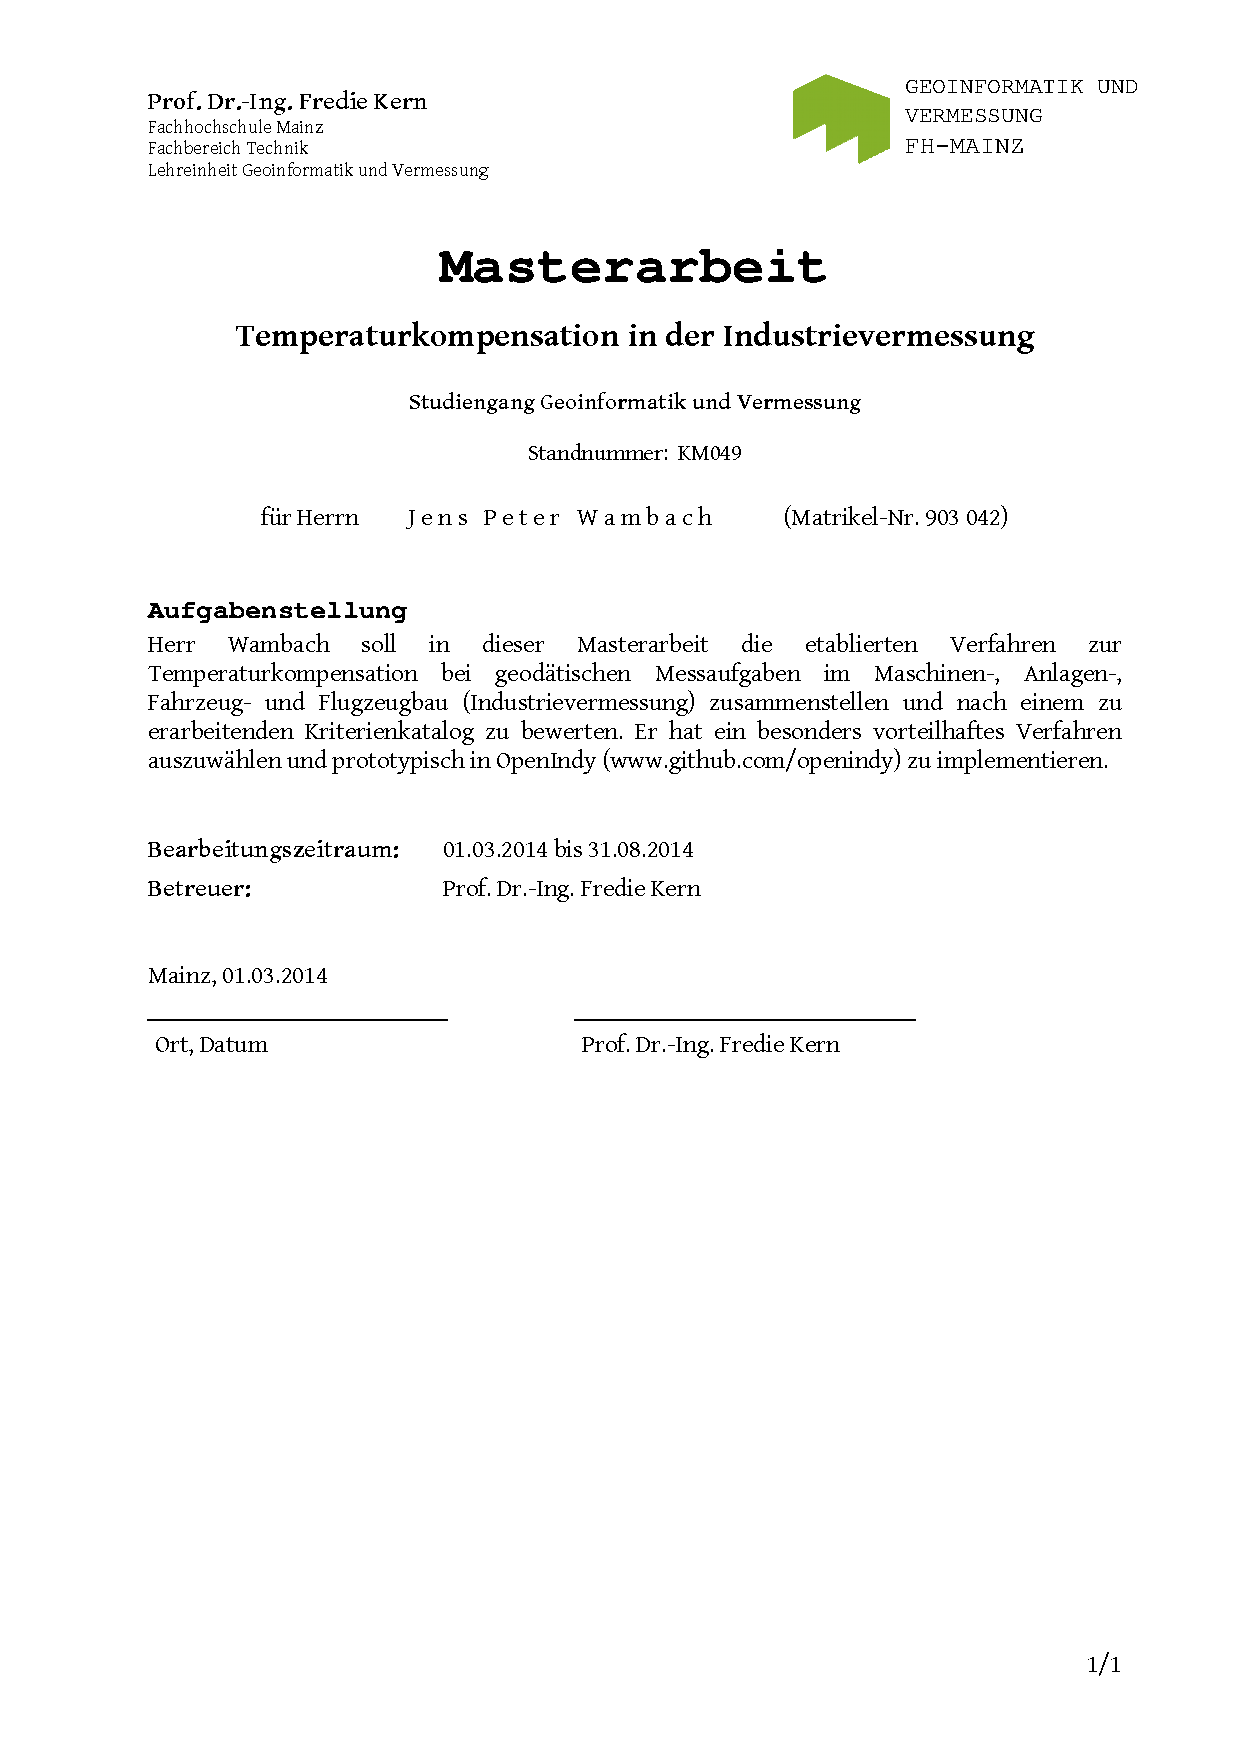
\includepdf[pages={1}]{bilder/aufgabenstellung_01.pdf}
\pagestyle{useheadings} % normale Kopf- und Fußzeilen für den Rest

\chapter*{Kurzfassung}\label{Kurzfassung}
\addcontentsline{toc}{chapter}{Kurzfassung}
\markboth{Kurzfassung}{Kurzfassung}

Ziel der Masterarbeit ist es ein Verfahren zur Temperaturkompensation in der Industrievermessung zu entwickeln. Der Schwerpunkt und Anwendungsbereich der Kompensation soll die thermische Ausdehnung des Messobjekts sein.\\ 
Als Grundlage des Verfahrens dient eine Zusammenstellung und Erarbeitung aktueller und kommerzieller Verfahren und Softwarelösungen für diese Problemstellung. Anhand dieser werden Kriterien für das neue Verfahren ermittelt und im späteren Verlauf der Entwicklung berücksichtigt.\\
Im Gegensatz zu den bereits existierenden Verfahren hat das neue Verfahren zur Temperaturkompensation den Unterschied, dass eine Kompensation der Messwerte nicht zum Koordinatenursprung des Messobjekts, sondern zu einem neu entwickelten und festzulegenden Ausdehnungsursprung durchgeführt wird.\\
Im Rahmen der Masterarbeit wurden zwei Verfahren entwickelt, die zur Kompensation verwendet werden können. Zum einen besteht die Möglichkeit die Ausdehnung des Messobjekts durch Messung der Objekttemperatur zu erfassen. Hierzu ist ebenfalls der Ausdehnungskoeffizient notwendig. Die andere Variante ermöglicht eine Erfassung und Kompensation der Ausdehnung durch Anwenden einer Transformation.\\
Die Verfahren und die Softwarelösung OpenIndy sind Open- Source, was eine Einsicht in die Algorithmik ermöglicht. Dies führt zu einer Transparenz der Verfahren, die je nach Anwendungsfall angepasst werden können.

\chapter*{Abstract}\label{Abstract}
\addcontentsline{toc}{chapter}{Abstract}
\markboth{Abstract}{Abstract}

The purpose of this master thesis is to develop a method for temperature compensation in industrial measurement. The main focus and area of application is the compensation of the thermal expansion of the part object.\\
The fundamental of the developed method is a compilation of modern and commercial methods and software solutions for temperature compensation used for this task. Based on this, criterias for the new method are determined and considered in the development of the method.\\
Other than the modern state of the art procedures, the here presented method for temperature compensation works different. The compensation of the measurement is not applied in direction of the origin of the part coordinate system, but in the direction of a newly developed origin of expansion that has to be determined.\\
As part of the master thesis, two procedures are developed that can be used to compensate the influence of the temperature. One procedure can capture the expansion of the part object by measuring the part temperature. In this procedure you also need to know the coefficient of thermal expansion of the part object. The other procedure can capture and compensate the expansion by applying a spatial transformation.\\
The methods and the software solution OpenIndy is open- source, what allows an insight in the algorithms. This leads in a transparency of the methods, that can also be adjusted for some special cases.


\chapter*{Erklärung}
Hiermit erkläre ich, dass ich die vorliegende Masterarbeit selbständig angefertigt habe. Es wurden nur die in der Arbeit ausdrücklich benannten Quellen und Hilfsmittel benutzt. Wörtlich oder sinngemäß übernommenes Gedankengut habe ich als solches kenntlich gemacht.\\

\vspace{3cm}
Ort, Datum\hrulefill \enspace Unterschrift\hrulefill\\

\tableofcontents
\listoffigures
\listoftables
%\listofalgorithms

\chapter{Überblick}\label{chap:Überblick}
\pagenumbering{arabic} % ab jetzt die normale arabische Nummerierung

Eine Große Rolle in der Industrievermessung spielen Präzisionsmessungen zur Fertigungs- und Qualitätskontrolle im Automobil-, Flugzeug- und Schienenfahrzeugbau. Dazu \cite{Moeser2007}: 
\begin{quotation}
\glqq Als Anfang der 50er Jahre die Ingenieurbauwerke immer größer und höher wurden, wurde der Begriff „Ingenieurvermessung“ geprägt. Er ist heute nach DIN 18710 definiert als: „Vermessung im Zusammenhang mit der Aufnahme, Projektierung, Absteckung und Überwachung von Bauwerken oder anderen Objekten“. \\
Ende der 80er Jahre kamen Präzisionsmessungen zur Fertigungs- und Qualitätskontrolle
beim Automobil-, Flugzeug- und Schienenfahrzeugbau hinzu. Damit wurde die „Industrievermessung“ mit Messaufgaben höchster Präzision im Nahbereich als Spezialgebiet der Ingenieurgeodäsie beschrieben. Parallel dazu entwickelte sich die rechnergestützte Koordinatenmessung im Maschinenbau mit „Methoden zur indirekten Bestimmung der gesuchten Maße auf dem Umweg über die aus einzelnen Punkten im Raum mittels analytischer Geometrie zu ermittelnden Formelemente, wie Punkt, Gerade, Ebene, Kreis, Zylinder.“\grqq
\end{quotation} 
Die Anforderungen an immer kleiner werdende Toleranzen für die produzierten Objekte stellen die Hersteller vor immer größer werdende Herausforderungen. Thermische Fehler haben die Genauigkeit der Produktionsmaschinen in vergangener Zeit beeinflusst \cite{Fletcher2005}. Durch das immer geringer werdende Fehlerbudget von nur einigen $10\mu m$ in modernen Fertigungen \cite{Ferger}, spielen die thermischen Fehler eine immer größer werdende Rolle, da diese die größte einzelne Fehlerquelle in der Produktion sind und bereits einen Großteil des Fehlerbudgets entsprechen, beziehungsweise in einigen Fällen das Fehlerbudget überschreiten. Bis zu 75\% der geometrischen Fehler von gefertigten Objekten können auf thermische Einflüsse zurückgeführt werden \cite{Mayr2012}. Aus diesem Grund ist eine Temperaturkompensation bei Messungen mit geringem Fehlerbudget unerlässlich \cite{Bryan1965}.\\
Durch die Temperaturkompensation wird der Einfluss der Temperatur, beziehungsweise der Einfluss des Temperaturunterschiedes zur Referenztemperatur (in der Regel $20^\circ\text{C} $) und die damit zusammenhängende Verformung des Messobjektes reduziert, kann jedoch nicht vollständig eliminiert werden \cite{Fletcher2005}. \\
Bereits existierende Ansätze, unterscheiden sich in ihrer Anwendbarkeit, Genauigkeit, sowie Kosten und Zeitaufwand. Zu den bereits existierenden Verfahren, die in den weiteren Kapiteln näher beschrieben werden, zählen die Erfassung der Temperatur des Messobjektes durch unterschiedliche Temperatursensoren, das Klimatisieren des Messraumes und somit des Messobjektes auf die vorgegebene Referenztemperatur und das Verwenden unterschiedlicher Materialien mit voneinander abweichenden Ausdehnungskoeffizienten.
Die Genauigkeiten der Verfahren hängen meist von den verwendeten Temperatursensoren, deren Genauigkeit zur Erfassung der Temperatur, der Position des Temperatursensors am Objekt und der Anzahl der verwendeten Temperatursensoren ab \cite{yuan1998} \cite{Mayr2012}. Meistens finden hier digitale Temperatursensoren ihren Verwendungszweck, da diese kostengünstig und ausreichend genau sind \cite{Fletcher2005}.\\
Problematisch ist nur die Bestimmung der tatsächlichen Temperatur des Messobjektes, weil häufig nur die Oberflächentemperatur gemessen werden kann. Jedoch kann die Temperatur nur wenige Zentimeter tiefer im Messobjekt von der gemessenen Temperatur abweichen, was direkten Einfluss auf das Ausdehnungsverhalten des Messobjekts hat. \\ Je nach Messobjekt besteht zum Teil auch gar nicht die Möglichkeit die Temperatur ausreichend genau zu bestimmen, da das Messobjekt nur gering bis gar nicht zugänglich ist.
Hinzu kommen Differenzen des angenommenen Ausdehnungskoeffizienten vom tatsächlichen Ausdehnungskoeffizient des Messobjektes. Dieser Effekt entsteht, wenn sich das verwendete Material des Messobjektes vom zur Kompensation angenommenen Material unterscheidet \cite{Bryan1965} \cite{Neumann08}. 


\chapter{Ziele}\label{chap:Ziele}

Ziel der Masterarbeit ist es Grundlagen der Wärmelehre und Ausdehnung von Objekten darzustellen, die bei derzeitigen Verfahren zur Temperaturkompensation Anwendung finden. Eine Auswahl derzeitiger Verfahren soll anhand theoretischer und praktischer Kriterien aufgeführt und verglichen werden. Beim Vergleich der Verfahren sollen Vorteile, sowie Nachteile der einzelnen Verfahren erarbeitet werden. Ebenso werden Einschränkungen in den Einsatzmöglichkeiten und Genauigkeiten der Verfahren gegenübergestellt. \\
Die erarbeiteten Vor- und Nachteile dienen als Kriterienkatalog für das zu implementierende Verfahren. Das zu entwickelnde Verfahren zur Kompensation der thermischen Ausdehnung von Messobjekten wird in OpenIndy\footnote{https://github.com/openindy/} implementiert.
Eine Verifizierung und Validierung der Algorithmik wird mit Hilfe einer praxisnahen Testmessung durchgeführt. In dieser Messung wird die Ausdehnung eines Testobjekts simuliert.\\
Da die Erfassung der tatsächlichen Objekttemperatur oft nicht möglich, oder nicht ausreichend genau durchführbar ist, soll eine der entwickelten Funktionen die Möglichkeit bieten eine Kompensation ohne Erfassung von Objekttemperatur und Material durchzuführen.\\
Ein zusätzliches Kriterium ist die Entwicklung der Funktionen und Algorithmik als Open- Source- Projekt, sodass diese transparent und nachvollziehbar sind. Es soll die Möglichkeit bestehen die Funktionalität für Spezialfälle zu erweitern und anzupassen.

\chapter{Temperatur und thermische Ausdehnung}\label{chap:TempAusdehnung}

Eine Ursache für die Ausdehnung von Körpern ist die Temperatur. Durch eine Abweichung der Temperatur von der Solltemperatur führt dies auch zu einer Abweichung in den Messwerten, die die kleinen Toleranzbereiche in der Industrievermessung überschreiten, oder einen Großteil dieses Bereiches in Anspruch nehmen \cite{Bryan1965}. \\
Jeder Körper, der erwärmt oder abgekühlt wird, dehnt sich in alle Richtungen aus, beziehungsweise schrumpft in allen Richtungen zusammen. Häufig ist hier jedoch nur die Längenänderung zur ursprünglichen Länge $l_{0}$ des Objektes von Interesse. Die neue Länge und die Temperaturdifferenz $\Delta\vartheta=\vartheta-\vartheta_{0}$ sind annähernd proportional zur ursprünglichen Länge \cite{Lindner2006}. Das Symbol $\vartheta$ repräsentiert die CELSIUS-Skala und T ist das Symbol für die KELVIN-Skala. Dies ist im weiteren Gebrauch der Formeln zu berücksichtigen, um die richtige Skala zu beachten \cite{Lindner2006}.\\
Der Längenausdehnungskoeffizient $\alpha$ ist der Proportionalitätsfaktor, der für das jeweilig vorliegende Material charakteristisch ist \cite{Lindner2006}.\\
Die Längenänderung 
\begin{equation}
\Delta l=\alpha l_{0}\Delta\vartheta
\label{eq:deltaL} 
\end{equation}
ergibt nach Umstellung der Formel den Längenausdehnungskoeffizienten
\begin{equation}
\alpha=\dfrac{\Delta l}{l_{0}\Delta\vartheta}
\end{equation}
Durch die material- und temperaturbedingte Längenänderung lässt sich die neue Gesamtlänge ermitteln
\begin{equation}
l=l_{0}+\Delta l = l_{0}(l+\alpha\Delta\vartheta)
\label{eq:gesamtlaenge}
\end{equation}

\newpage
\begin{figure}[h]
	\label{fig:laengenaenderung}
	\centering
		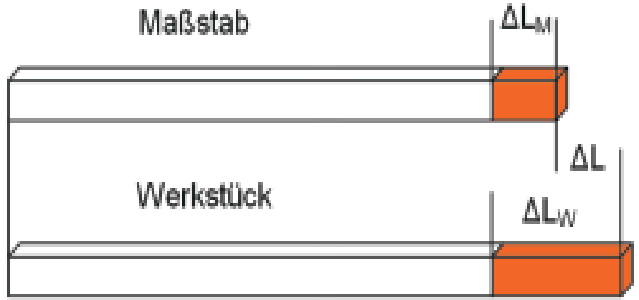
\includegraphics[scale=1.5]{bilder/ausdehnung}
	\caption[temperaturbedingte Längenänderung]{Ausdehnung von Werkstück und Maßstab eines Koordinatenmessgeräts.\protect\footnotemark}
\end{figure}
\footnotetext{Quelle: \cite{Ferger}}

\section{Ausdehnung von Materialien}\label{chap:Ausdehnung}

Ursache für die Ausdehnung des Messobjektes und die Abweichung der Temperatur ist, die Bestimmung der Sollwerte in einem klimatisierten Messlabor.\\
Die Ist-Erfassung des Objektes zur Kontrolle hingegen erfolgt meistens am Fertigungsort, sodass starke Abweichungen zu den Laborbedingungen und zur Referenztemperatur vorzufinden sind \cite{Ferger}.
Eine Möglichkeit der temperaturabhängigen Ausdehnung entgegen zu wirken, wäre es den Fertigungsort zu klimatisieren und laborähnliche Verhältnisse zu erzeugen. Dieses Vorgehen ist jedoch in den meisten Fällen zu aufwändig und kostspielig \cite{Bryan1965}.\\
Ebenso werden thermische Fehler durch thermische Verzerrungen und Ausdehnungen von Maschinenteilen durch interne und externe Wärmequellen, Motoren, hydraulische Systeme, Halterungen und der Umgebungstemperatur beeinflusst \cite{yuan1998}.\\
In \cite{Ferger} sind einige Maßnahmen genannt, die eine Temperaturkorrektur sicherer und wirksamer machen. Diese beziehen sich hauptsächlich auf Messungen mit Koordinatenmessgeräten, sind jedoch auch in anderen Verfahren anwendbar.
\begin{small}
	\begin{itemize}
		\item Möglichst nur geringe Temperaturänderungen zulassen
		\item Zugluft vermeiden
		\item Bei schnellen Temperaturänderungen Geräte umhausen
		\item Wärmequellen konstant in Betrieb halten
		\item Geräte mindestens im Abstand von 1m zu den Wänden installieren
		\item Fußboden thermisch isolieren
		\item Keine direkte Sonneneinstrahlung zulassen
		\item Das Messobjekt sollte die Umgebungstemperatur angenommen haben
		\item Berührung der Teile mit den Händen vermeiden bzw. Handschuhe tragen
		\item Konstante Temperatur während eines Messzyklus sicherstellen
		\item Bei langen Messzyklen, Driftkontrolle durch Überprüfung des Referenzkoordinatensystems durchführen
	\end{itemize}
\end{small}

\section{Liste von Ausdehnungskoeffizienten}\label{sec:ListevonAusdehnungskoeffizienten}

Im nachfolgenden ist eine Tabelle mit Ausdehnungskoeffizienten einiger fester Stoffe abgebildet. Die Angaben beziehen sich auf einen Gültigkeitsbereich von $0^\circ\text{C}$ bis $100^\circ\text{C}$. Bei größeren Temperaturbereichen sind diese Angaben nicht mehr ausreichend genau bestimmt, sodass man mit der Annahme, dass $\alpha$ temperaturabhängig ist, zu einem erweiterten Term zur Berechnung des Koeffizienten gelangt. Auf diese Weise lässt sich das wirkliche Verhalten der Körper bei höheren Temperaturen besser annähern \cite{Lindner2006}. Die Angabe des Gültigkeitsbereiches der Ausdehnungskoeffizienten erfolgt, um die lineare Beziehung der Längenänderung im spezifizierten Bereich anwenden zu können.
\begin{table}[h]
	\centering
	\caption[Längenausdehnungskoeffizienten]{Längenausdehnungskoeffizienten einiger fester Stoffe in $10^{-6}m/K*m(0...100^\circ\text{C})$\protect\footnotemark}
	\begin{tabular}{|c|c||c|c|}
		\hline
		Aluminium & 24 & Platin & 9 \\
		\hline
		Blei & 30 & Wolfram & 4.5 \\
		\hline
		Eisen, rein & 12 & Glas & 6...9 \\
		\hline
		Grauguß & 9 & Quarzglas & 0.54 \\
		\hline
		Stahl V2A & 16 & Invar (64\% Fe, 36\% Ni) & 2 \\
		\hline
		Konstantan & 15 & Suprainvar (63\% Fe, 32\% Ni, 5\% Co, 0.3\% Mn) & 0.1...0.5 \\
		\hline
		Kupfer & 17 & Kalkstein & 4 \\
		\hline
		Messing & 18 & Jenaer Pyrexglas & 3.3 \\
		\hline
		Zink & 27 & Normalbeton bei $25^\circ\text{C}$\protect\footnotemark & 12 \\
		\hline
		Stahlbeton bei $25^\circ\text{C}$\footref{ftn:stoecker} & 10...15 & & \\
		\hline
	\end{tabular}
\label{tab:ausdehnungskoeffizienten}
\vspace{-1cm}
\end{table}
\addtocounter{footnote}{-1}\footnotetext{Quelle: \cite{Lindner2006}}
\stepcounter{footnote}\footnotetext{Quelle: \cite{Stoecker2007}\label{ftn:stoecker}}
\newpage

Wie Tabelle \ref{tab:ausdehnungskoeffizienten} zu entnehmen ist, haben Beton und Stahl thermische Ausdehnungskoeffizienten in der selben Größenordnung. Da in der Industrie häufig diese beiden Elemente kombiniert sind, zum Beispiel Stahlkonstrukte auf Betonfundamenten oder mit Befestigungen an Betonsäulen, ist hier eine größtenteils homogene Ausdehnung anzunehmen. Da in der Praxis und auch bei kommerziellen Messprogrammen, die in der Industrievermessung Anwendung finden, in der Regel nur ein Material für die gesamte Temperaturkompensation gewählt wird, bzw. gewählt werden kann, so hat die Entscheidung des Materials für die beiden genannten Fälle keinen signifikanten Einfluss auf die Temperaturkompensation.\\ 

Zur genaueren Bestimmung der Ausdehnungskoeffizienten, muss die lineare Beziehung aus Gleichung \ref{eq:deltaL} erweitert werden. \glqq[...], daß der Ausdehnungskoeffizient $\alpha$ selbst wieder eine lineare Funktion der Temperatur ist:\grqq \cite{Lindner2006}.\\
Somit ergibt sich:
\begin{equation}
\alpha = \alpha_{0}+\tilde{\beta}\Delta\vartheta
\end{equation}
und die neue Gleichung für die Gesamtlänge
\begin{equation}
l=l_{0}[1+\alpha_{0}\Delta\vartheta+\tilde{\beta}(\Delta\vartheta)^{2}]
\end{equation}
Der Einfluss von $\tilde{\beta}$ ist sehr gering und entspricht bei den in Anwendungen der Industrievermessung üblichen Temperaturen von unter $100^\circ\text{C}$ Korrekturen im Submikrometerbereich. Dessen Einfluss darf vernachlässigt werden, sodass die lineare Beziehung aus Gleichung \ref{eq:gesamtlaenge} angewandt werden kann \cite{Lindner2006}. Nachfolgend eine Bestimmung des Ausdehnungskoeffizienten erster und zweiter Ordnung anhand von Platin \cite{Lindner2006}:
\begin{quotation}
So wurden z.~B. bei Platin die Werte $\alpha_{0}=8,5*10^{-6}1/K \; und \; \tilde{\beta}=3,5*10^{-9}1/K^{2}$ ermittelt. Hieraus ist zu ersehen, daß der Koeffizient $\tilde{\beta}$ erst bei höheren Temperaturen ins Gewicht fällt. \cite{Lindner2006}
\end{quotation}
Um die Notwendigkeit der Angabe des Gültigkeitsbereiches der Ausdehnungskoeffizienten noch einmal zu verdeutlichen, sind nachfolgend noch einmal einige Materialien in den beiden genannten Gültigkeitsbereichen gegenübergestellt. So hat zum Beispiel Stahl (V2A) bei $25^\circ\text{C}$ einen Ausdehnungskoeffizienten von $\alpha = 16.0\mu m$. In der verallgemeinerten Angabe nach \cite{Lindner2006} hat Stahl ebenfalls einen Koeffizienten von $16.0\mu m$. Zink hingegen hat bei $25^\circ\text{C}$ einen Ausdehnungskoeffizienten von $\alpha =  30.2 \mu m$, in der Verallgemeinerung jedoch $27.0 \mu m$. \\
Dieser Gegenüberstellung kann man entnehmen, dass die Angabe der Ausdehnungskoeffizienten für einen Temperaturbereich zwar den Vorteil hat, dass man sie linear verwenden kann, jedoch auch den Nachteil, dass sie eine Ungenauigkeit in die Angabe des exakten Wertes eines Materials einbringt. Ein Abgleich der aufgeführten Materialien der Quellen zeigt jedoch, dass die Abweichungen im Mikrometer bis Submikrometerbereich liegen.

\section{Wärmeleitfähigkeit}\label{sec:Wärmeleitfähigkeit}

Neben der durch Temperatur bedingten Ausdehnung von Materialien, ist auch die Wärmeleitfähigkeit von Stoffen in einigen Fällen der Industrievermessung von Bedeutung und muss beachtet werden.\\
Die Zuführung oder das Entziehen von Wärmeenergie an einem Objekt, führt zu einer Änderung seiner Temperatur. Die benötigte Wärmemenge hängt von der Anfangstemperatur des Objektes, seiner Masse und der Art des zu erwärmenden Stoffes ab.
Des weiteren sind in \cite{Lindner2006} Varianten der Ausbreitung für Wärmeenergie genannt. Im nachfolgenden sind drei der Varianten zu finden, die für die Industrievermessung relevant sind.\\
\newline
\textbf{Wärmeleitung:}\\
Ausbreitung von Wärme innerhalb eines Körpers\\
\newline
\textbf{Wärmeübergang:}\\
Übertragung von Wärmeenergie bei Berührung von Körpern verschiedener Temperatur\\
\newline
\textbf{Wärmestrahlung:}\\
Abstrahlung von Wärmeenergie auch durch den leeren Raum\\
\newline

Diese drei Eigenschaften werden im nachfolgenden noch in einigen Anwendungsbeispielen gefunden, bei denen diese zu beachten sind und Verwendung finden.\\

Hat ein System verschiedene Temperaturen, so strebt es das thermische Gleichgewicht an. Es findet ein Wärmestrom von der wärmeren zur kälteren Stelle statt \cite{Lindner2006}. Die Wärmeleitfähigigkeit $\lambda$ ist, ebenso wie der thermische Ausdehnungskoeffizient, materialabhängig.
Im nachfolgenden einige Wärmeleitfähigkeitswerte.
\begin{table}[h]
\centering
\caption[Wärmeleitfähigkeit]{Wärmeleitfähigkeit in W/(mK)\protect\footnotemark}
	\begin{tabular}{|c|c||c|c||c|c|}
		\hline
		Silber & 418.6 & Blei & 35.0 & Holz & 0.2 \\
		\hline
		Kupfer & 377.8 & Beton & 1.3 & Aluminium & 209 \\
		\hline
		Luft bei $0^\circ\text{C}$ & 0.023 & Stahl & 41.7 ...55.6 & Ziegelmauer & 0.81 \\
	\hline
	\end{tabular}
\label{tab:wärmeleitfähigkeit}
\end{table}
\footnotetext{Quelle: \cite{Lindner2006}}

Wie Tabelle \ref{tab:wärmeleitfähigkeit} zu entnehmen ist, hat Beton eine sehr geringe Leitfähigkeit. Beton benötigt also eine große Zeitspanne, bis er sich erhitzt oder abkühlt. Stahl hingegen hat einen deutlich höheren Wertebereich, erhitzt sich somit schneller, und dehnt sich folglich schneller aus als Beton.\\
Die Wärmeleitfähigkeit ist abhängig von der Temperatur und es sind zwei Fälle zu unterscheiden.
Zum einen existiert die \textbf{stationäre Wärmeleitung}, bei der zwei Temperaturen an den beiden Endflächen, deren Abstand \textit{l} ist, konstant gehalten werden. Zwischen ihnen herrscht ein konstantes Temperaturgefälle. Dies entspricht einem Dampfkessel, dessen Innentemperatur konstant gehalten wird, und die Außentemperatur ebenfalls gleich bleibt \cite{Lindner2006}.\\
Zum anderen gibt es die \textbf{nichtstationäre Wärmeleitung}, bei der eine Seite des Körpers wärmer ist, als die andere. Im Laufe der Zeit wird sich der Temperaturunterschied ausgleichen und der Körper nimmt eine einheitliche Temperatur an. Das Temperaturgefälle ist weder örtlich noch zeitlich konstant, maßgebend ist jedoch die Wärmeleitfähigkeit des Materials \cite{Lindner2006}.\\
In der Produktion ist in der Regel meistens die nichtstationäre Wärmeleitfähigkeit vorzufinden. Da die Objekte häufig zwischen verschiedenen Standorten transportiert werden und ständig neuen Temperaturen ausgesetzt sind, findet an jeder Position ein Wärmeausgleich statt. Dieser benötigt jedoch, je nach Material, eine gewisse Zeit, und ist bei Messungen zu berücksichtigen. \\
In diesen Fällen sind die oben genannten Ausbreitungsvarianten der Wärmeenergie wiederzufinden. Nach dem das Objekt einer neuen Temperatur ausgesetzt ist, nimmt es Wärmeenergie der Umgebungstemperatur, des Bodens usw. auf. Diese wirkt sich auf die Temperatur des Objektes aus (Wärmeleitung), und verursacht ein Gleichgewicht der Temperaturen. Dieser Prozess ist jedoch je nach Temperaturunterschied und Materialien sehr zeitintensiv. \\
Die dritte Variante der Ausbreitung von Wärmeenergie, die Wärmestrahlung, wird in vielen Fällen zur berührungslosen Erfassung der Objekttemperatur verwendet.

\chapter{Temperaturerfassung und Sensoren}\label{chap:Temperaturerfassung}

Um Temperaturkompensation in der Messaufgabe anwenden zu können, bedarf es Kenntnis über den Ausdehnungskoeffizienten und die Temperatur des zu kompensierenden Objektes. Da der thermische Ausdehnungskoeffizient so genau wie möglich sein sollte, muss man das Material des Objektes genau kennen und den passenden Koeffizienten zum Material wählen. Hierbei ist auch darauf zu achten, dass der Ausdehnungskoeffizient für den Temperaturbereich gültig ist, da sonst weitere Ungenauigkeiten Einfluss auf die Temperaturkompensation erhalten.\\
Zusätzlich muss auch die Temperatur des Messobjektes bekannt sein. Diese sollte möglichst genau der Kerntemperatur des Objektes entsprechen, um die tatsächliche Ausdehnung so gut wie möglich repräsentieren zu können. Ein großes Problem ist, dass bei unzureichend genau erfasster Temperatur, oder bei der Wahl eines falschen Ausdehnungskoeffizienten die Messaufgabe durch Anwendung der Temperaturkompensation verschlechtert werden kann \cite{eschelbach2007}. Des weiteren ist es theoretisch notwendig, dass sich das Messobjekte in einem thermischen Gleichgewicht mit seiner Umgebung befindet, sodass sich die Kerntemperatur während des Messens nicht verändert.\\
In der Praxis ist es jedoch meistens nicht möglich diese Anforderungen umzusetzen, weshalb einige zusätzliche Maßnahmen getroffen werden müssen. \\
In vielen Fällen ist es nicht möglich, die Raumtemperatur ohne großen Aufwand auf einer konstanten Temperatur zu halten, da durch Belüftungen, Fensterfronten oder auch durch die Raumbeleuchtung  Teile der Raumluft erwärmt, oder abgekühlt werden, was zu einer Schwankung im Temperaturfeld führt. Diese Schwankung wirkt sich direkt auf die Präzisionsmessungen aus \cite{eschelbach2007}.\\
In der Regel findet eine örtliche Bestimmung der Temperatur statt. Je nach Anforderung und Gegebenheiten der Messaufgabe findet die Temperaturbestimmung örtlich durch Bestimmung der Umgebungstemperatur, oder durch Erfassung der direkten Objekttemperatur statt. Wenn die Erfassung der Umgebungstemperatur ausreichend ist, sollten die Genauigkeitsanforderungen geringer sein, da größere Abweichungen von der tatsächlichen Objekttemperatur zu erwarten sind, oder das Objekt sollte sich im thermischen Gleichgewicht mit der Umgebungstemperatur befinden. Wesentlich komplexer wird die Erfassung einer repräsentativen Temperatur jedoch, wenn sich die Messung nicht in einem kleinen Bereich des Raumes begrenzt \cite{eschelbach2007}.\\
Das Temperaturfeld sollte während der Messung weitestgehend stabil bleiben, andernfalls muss, bei Überschreitung eines Grenzwertes, die Temperatur neu erfasst werden und mit in die Kompensation einfließen. \cite{eschelbach2007} schlägt bei einer mobilen Feldprüfung eines Lasertrackers direkt vor der Projektmessung einen Grenzwert von $0,2^\circ\text{C}/h$ vor.\\
Die Temperatur kann auf unterschiedliche Weise erfasst werden. Hierzu stehen berührungslose Sensoren oder Kontaktsensoren zur Verfügung. Die Wahl des Sensors hat unmittelbar Auswirkungen auf die Messzeit zur Erfassung der Temperatur, die Genauigkeit der Messung und den Aufwand, um die Messung durchzuführen.

\section{Kontaktthermometer}\label{sec:Kontaktthermometer}

Kontaktthermometer werden mit dem zu messenden Objekt in Kontakt gebracht, sodass der Thermometer mit der Objekttemperatur in ein thermisches Gleichgewicht überführt wird. Die Temperatur ist dann am Thermometer abzulesen. Bei Kontaktthermometer unterscheidet man zwischen mechanischen Thermometern, die eine Temperaturabhängigkeit des Volumens von Stoffen zu Grunde legen, und elektrischen Thermometern, die die Temperaturabhängigkeit des elektrischen Widerstandes, oder eine Kontaktspannung zwischen zwei verbundenen Metallen zu Grunde legen. \\
Kontaktthermometer haben einen Anwendungsbereich bis 1500 Kelvin \cite{Siddiqi}. Bei Kontaktthermometern ist auf die vom Material abhängige Anzeigeverzögerung zu achten, da dadurch eventuell eine steigende Temperatur am Thermometer angezeigt wird, obwohl das Objekt bereits abkühlt \cite{Siddiqi}.

\paragraph{Flüssigkeits- Gas- Thermometer}\label{par:fluessiggasthermo}

 gehören zu den Ausdehnungsthermometern und beruhen auf der Ausdehnung der darin befindlichen Flüssigkeit. Der Anwendungsbereich dieses Typs von Thermometer liegt zwischen $-35$ und $625^\circ\text{C}$ und hat eine Empfindlichkeit von bis $0,01^\circ\text{C}$. Zur Messung der Temperatur sind keine weiteren Hilfsmittel nötig, und die Temperatur kann direkt an der Messstelle abgegriffen werden \cite{Siddiqi}.

\paragraph{Widerstandsthermometer}\label{par:widerstandsthermo}

 basieren auf der Messung eines elektrischen Widerstands. Dieser ist temperaturabhängig, und wird durch die Objekttemperatur erhitzt oder abgekühlt. Ihre Messgenauigkeit beträgt unter Laborbedingungen bis zu $10^{-3 \circ}\text{C}$.\\
Weitere Vorteile dieser Art von Thermometer sind ihr robuster Aufbau und eine gute Reproduzierbarkeit. Ebenso lässt sich die Temperatur aus großer Entfernung zum Objekt ablesen \cite{Siddiqi}. Ein häufig verwendeter Sensor dieser Kategorie ist der Widerstandsthermometer Typ Pt 100.

\paragraph{Thermoelemente}\label{par:thermoelemente}

 arbeiten nach dem Prinzip, dass zwischen zwei miteinander verlötet oder verschweißten Metallen eine Thermospannung auftritt, welche material- und temperaturabhängig ist. 
Bei Temperaturunterschied ist eine Spannung zu messen, die exakt die Temperaturdifferenz widerspiegelt. Ein Problem hierbei ist, dass eine der beiden Kontaktstellen auf einer konstanten Temperatur gehalten werden muss, um die tatsächliche Objekttemperatur erfassen zu können \cite{Siddiqi}.

\section{Infrarot}\label{sec:infrarot}

Anhand ausgesandter elektromagnetischer Wellen eines Körpers, ist es möglich die Temperatur von diesem zu erfassen. Die Wellen sind temperaturabhängig und liegen bis $600^\circ\text{C}$ im unsichtbaren langwelligen Bereich. Mit Hilfe moderner Kameras und Messeinrichtungen, ist es möglich die Strahlung elektronisch zu verarbeiten und die unterschiedlichen Temperaturbereiche auf einem Bildschirm farblich zu unterscheiden \cite{Lindner2006}.\\
Vorteil dieser Methode zur Erfassung der Temperatur ist die zerstörungsfreie und kontaktlose Messung. Aufgrund handlicher Sensoren und nur sehr kurzen Messzeiten ist die Messung auch an heißen oder nur schwer zugänglichen Stellen und Objekten möglich \cite{optris}. Hand- Infrarotthermometer haben einen Anwendungsbereich von $-32$ und $530^\circ\text{C} $ mit einer Genauigkeit von $\pm$ 1\% bzw. $\pm$ $1^\circ\text{C}$ und einer Auflösung von $0,1^\circ\text{C}$. Die erfasste Temperatur entspricht jedoch nur der Oberflächentemperatur des Objektes und nicht der Kerntemperatur. Mit einigen Kontaktthermometern, die in Bohrungen am Objekt angebracht werden, lässt diese sich hingegen bestimmen. Ebenso ist bei Infrarotsensoren zu beachten, dass von der Umgebung reflektierte und durch das Objekt durchgelassene Infrarotstrahlung, sowie der Einfluss von in der Nähe befindlichen Wärmequellen, mit erfasst werden kann und in den Messwert mit einfließt \cite{optris}.\\
Bei der Verwendung von Hand- Infrarotthermometern ist zu beachten, dass das zu messende Objekt größer als der Messbereich des Sensors ist, sodass keine Störgrößen aus umgebenden Strukturen, eventuell aus anderem Material, in die Messung mit einfließen. Dies wird je nach Sensor durch verschiedene visuelle Kennzeichnungen des Messbereiches unterstützt. Durch vergrößern oder verringern des Abstandes zu Messobjekt wird der Messbereich angepasst.
\begin{figure}[h]
	\label{fig:infrarotMessbereich}
	\centering
		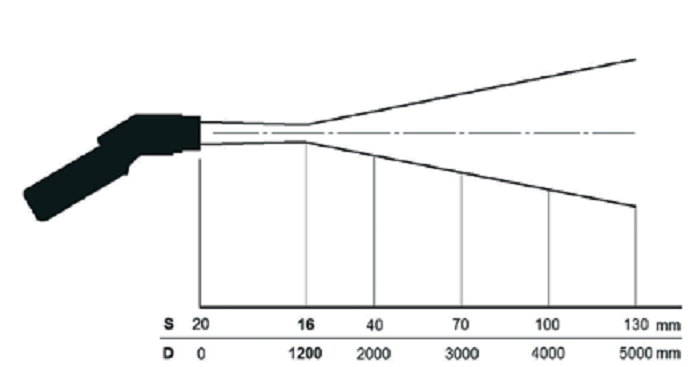
\includegraphics[scale=2.0]{bilder/infrarotMessbereich}
	\caption[optisches Diagramm eines Infrarotsensors]{optisches Diagramm eines Infrarotsensors\protect\footnotemark}
\end{figure}
\footnotetext{Quelle: \cite{optris}}

Hand- Infrarotthermometer werden zur schnellen Erfassung und Auswertung von lokalen Temperaturen verwendet.
In Fertigungslinien werden oft stationäre Infrarotsensoren und Infrarotkameras zur Qualitätssicherung verwendet.

\chapter{Anwendungsbeispiele der Temperaturkompensation}\label{chap:anwendungen}

Um das zu erarbeitende Verfahren der Temperaturkompensation entwickeln und in OpenIndy implementieren zu können, wurde nach aktuellen theoretischen und praktischen Ansätzen zur Temperaturkompensation recherchiert. Der Schwerpunkt hierbei lag auf den verwendeten Sensoren und Methoden zur Temperaturerfassung, sowie zur Bestimmung des Ausdehnungskoeffizienten und der Ausdehnung. Ein weiteres Augenmerk wurde auf die Anwendung der Kompensation und die resultierenden Ergebnisse gelegt, um den Einfluss und die Relevanz der Temperaturkompensation zu ermitteln und aufzuzeigen. Zudem sollten die Verfahren im Bereich der mobilen Messtechnik anwendbar sein, was bedeutet, dass so wenig wie möglich zusätzliche Sensorik benötigt werden sollten, sowie leicht und schnell auswertbar sein sollten.\\ 
Aus den nachfolgend vorgestellten Verfahren sollen Vor- und Nachteile erarbeitet werden, die im zu entwickelnden Verfahren umgesetzt werden.\\
Bei den nachfolgend vorgestellten Anwendungsbeispielen handelt es sich um Anwendungen in der mobilen Messtechnik, dem Flugzeugbau, aus dem Bereich der Koordinatenmessgeräte (KMG) und Werkzeugmaschinen. Zusätzlich sind einige Theorien und Versuche unter Laborbedingungen enthalten.

\section{Permanentüberwachung des 20m VLBI- Radioteleskops an der Fundamentalstation in Wettzell}\label{sec:teleskop}

Das am Geodätischen Observatorium in Wettzell eingerichtete Monitoringsystem zur Überwachung des 20m VLBI- Radioteleskops soll eventuell auftretende Deformationen, die unter anderem durch Temperaturänderungen hervorgerufen werden, detektieren und analysieren \cite{losler2010}. Diese Deformationsanalyse dient zur Überwachung von Referenzpunkten verschiedener Raumverfahren, wie beispielsweise der Very Long Baseline Interferometry (VLBI), um deren angestrebte Submillimetergenauigkeit sicher zustellen.\\
Zur Erfassung der Daten wurde der Tachymeter Leica TCA2003 und der Datenlogger MSR145W gewählt, da diese Kombination ein preisgünstiges Equipment darstellt und mehrere der Datenlogger an verschiedenen, als kritisch erkannten Bereichen, aufgestellt werden können, um eine hohe Repräsentativität zu erreichen. Zusätzlich wurden vier der im Monument verbauten Temperatursensoren zur Datenerfassung verwendet \cite{losler2010}.\\
Während des gesamten Überwachungszeitraumes wurden diverse Referenz- und Objektpunkte am Radioteleskop gemessen, die Rückschlüsse auf dessen Position liefern sollen. Aufgrund temperaturbedingter Ausdehnungen der Teleskopkabine muss hier eine Temperaturkompensation stattfinden. Hierzu ist jedoch die Objekttemperatur erforderlich, welche nicht bekannt ist. Deshalb wurde die Temperatur aus der Umgebungstemperatur und den Messwerten aus den im Monument verarbeiteten Sensoren abgeleitet.
\begin{figure}[h]
	\label{fig:Kabinenausdehnung}
	\centering
		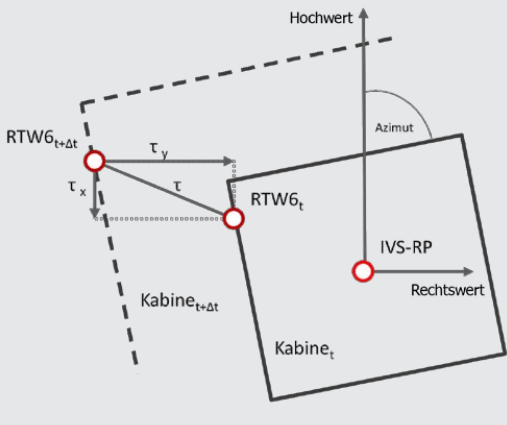
\includegraphics[scale=2.0]{bilder/Kabinenausdehnung}
	\caption[Schematische Darstellung der Teleskopkabinenausdehnung und deren Korrektur]{Schematische Darstellung der Teleskopkabinenausdehnung und deren Korrektur\protect\footnotemark}
\end{figure}
\footnotetext{Quelle: \cite{losler2010}}

\newpage
Der durch \cite{losler2010} aufgewiesene Einfluss der thermischen Ausdehnung auf die Position der Referenzpunkte zeigt, dass diese nicht vernachlässigbar ist, denn bei bereits $2^\circ\text{C}$ Abweichung der Objekttemperatur, findet eine Verschiebung um von $\Delta q = 0,05mm $ statt.


\section{Koordinatenmessgeräte und Messobjekt}\label{sec:KMG}

Koordinatenmessgeräte werden heutzutage nicht mehr ausschließlich in speziellen, klimatisierten Prüflaboren verwendet, sondern finden direkt am Ort der Fertigung Verwendung, was bedeutet, dass die Temperaturen unter Umständen stark von der Referenztemperatur von $20^\circ\text{C}$ abweichen.\\
Dies stellt Hersteller und vor allem Anwender vor zusätzliche Voraussetzungen, um die zum Teil hohen Genauigkeitsanforderungen an die gefertigten Objekte von wenigen $10\mu m $ einzuhalten \cite{Ferger}.\\
Bei Anwendung von Koordinatenmessgeräten am Ort der Fertigung, hat die Temperatur des Raumes einen großen Einfluss auf die Objekttemperatur und dessen Ausdehnung, sowie auf das KMG selbst, und die Ausdehnung dessen Maßstäbe und anderen Teilen.
Handelt es sich um ein \glqq thermisch stabiles KMG\grqq \cite{Neumann08}, so bezieht sich die Kompensation nur auf das Messobjekt, da die Einflüsse auf das KMG in der Spezifikation enthalten sind. Ist dies nicht der Fall kann eine Kompensation aufwändig oder fast unmöglich werden \cite{Neumann08}. \\
Zur Kompensation erfordert es genaue Angaben der Temperaturen der Maßstäbe, sowie der Objekttemperatur. Hierzu werden im Gerät verbaute Sensoren, als auch Kontaktsensoren verwendet, die die Temperatur des KMG und des Messobjektes erfassen sollen.\\
Des weiteren müssen die Ausdehnungskoeffizienten der Maßstäbe, als auch des Objektes bekannt sein. Auch eine Schätzung des Ausdehnungskoeffizienten des Messobjektes führt zu einer Reduzierung der Längenmessabweichung durch thermische Ausdehnung. Dies ist vor allem bei großen Bauteilen bemerkbar, da die Längenmessabweichung durch thermische Ausdehnung der größte Fehlereinfluss ist \cite{Ferger}.\\
Die Notwendigkeit und auch Komplexität einer Simulation aller Fehlereinflüsse, die auf ein Koordinatenmessgerät und das Messobjekt wirken können, wird von \cite{baldwin2007} näher erläutert und anhand einiger Beispiele dargestellt.\\
Auch dem Beispiel von \cite{Hernla2006} ist zu entnehmen, dass der thermische Einfluss auf KMG und Messobjekt einen großen Einfluss hat. Hier wird als praktische Anwendung ein Bohrlochdurchmesser bestimmt. Hierzu wird ein Kreis am Messobjekt erfasst. Bei der Erfassung und Ausgleichung des Formelements werden Einmessung des Tasters, die Tasteranlagekorrektur und der thermische Einfluss auf KMG und Messobjekt berücksichtigt. Das Fazit dieser Messung ist, dass die Temperatur des Werkstückes und der Maßstäbe den größten Einfluss auf das Ergebnis haben, und nur durch eine genauere Erfassung oder durch Klimatisierung des Messraumes zu reduzieren ist \cite{Hernla2006}.\\
In einigen speziellen Fällen ist es möglich die Temperatur des Werkstücks und der Maßstäbe aus Erfahrungswerten und Temperaturaufzeichnungen früherer Messungen abzuleiten \cite{Hernla2008}.\\
In Verbindung mit dem Temperatureinfluss, hat auch die Ausrichtung und der Abstand des Messobjekts zum Ursprung Einfluss auf das Ergebnis \cite{Hernla2013}.
\begin{quotation}
Der  Temperatureinfluss ist dann am stärksten, wenn der Abstand vom Koordinatenursprung am größten 
ist und die Auswerterichtung etwa zum Koordinatenursprung zeigt. \cite{Hernla2013}
\end{quotation}
Um ein reproduzierbares Bezugssystem zu haben, werden bei der Verformungsanalyse in \cite{Hernla2013} die zu messenden Sitzpolsterungen vor und nach der Belastung in eine Vorrichtung eingespannt und gemessen. 

\section{Werkzeugmaschinen und Objekt}\label{sec:Werkzeugmaschine}

Ebenso wie Koordinatenmessgeräte sind auch Werkzeugmaschinen Umgebungstemperaturen abweichend von $20^\circ\text{C}$ ausgesetzt. Neben dem Einfluss der Umgebungstemperatur, wirken hier auch noch interne Wärmequellen durch Motoren, Gelenke und anderen Wärme produzierenden Teile auf die 3D Genauigkeit. Diese Einflüsse sind zu kompensieren \cite{yuan1998}.\\
Die Kompensation kann hier online, d.h. während der Produktion erfolgen. Alternativ kann sie offline durchgeführt werden, also vor der Produktion des nächsten Fertigungsstücks. Eine offline Kompensation lohnt sich nur bei Massenproduktionen, bei denen das Werkstück nicht ständig wechselt \cite{yuan1998}. \\
Die Kompensation wird hier über einen Controller und verschiedene Modelle zur Kompensation aller Fehlereinflüsse geregelt \cite{mekid2010}. Zur Kompensation werden diverse Eingangsgrößen, unter anderem auch Temperaturmessungen benötigt. Temperaturquellen einer Werkzeugmaschine sind schwer zu lokalisieren und zu erfassen und ändern sich abhängig vom Zustand der Maschine \cite{mekid2010}. Um die Genauigkeit der Temperaturerfassung zu steigern, werden mehrere Temperatursensoren und Simulationen zur Ermittlung der optimalen Positionen für die Sensoren verwendet. Durch die in der Simulation ermittelten Sensorpositionen ist es möglich einige Sensoren an nicht repräsentativen Stellen der Werkzeugmaschine zu sparen.\\
Einige moderne Werkzeugmaschinen nutzen die Möglichkeit der Temperaturerfassung über Infrarotstrahlung (Kapitel \ref{sec:infrarot}) und verwenden Infrarotkameras zur flächenhaften Erfassung des Temperaturfeldes von Werkstück und Maschine, was zu besseren Ergebnissen bei der Kompensation führt.
\begin{figure}[h]
	\label{fig:WMInfrarot}
	\centering
		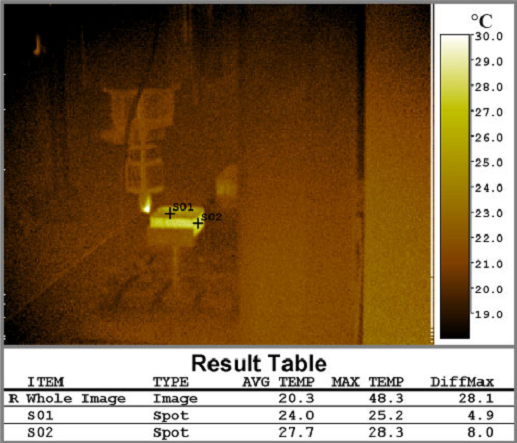
\includegraphics[scale=2.0]{bilder/WMInfrarot}
	\caption[Wärmebild von Schneidewerkzeug und Werkstück]{Wärmebild von Schneidewerkzeug und Werkstück\protect\footnotemark}
\end{figure}
\footnotetext{Quelle: \cite{mekid2010}}
Durch die flächenhafte Erfassung der Temperatur durch eine Infrarotkamera oder mehrere Temperatursensoren, ist es möglich die thermischen Fehler für jedes Element der Werkzeugmaschine zu ermitteln und zu korrigieren.\\
Eine weitere Möglichkeit den thermischen Einfluss zu verringern ist die Anwendung von Finite-Element-Modellen. Dieser Ansatz ist kostspielig und liefert nur unzureichend genaue Ergebnisse, da Randbedingungen, wie beispielsweise exakt lokalisierte Wärmequellen zuvor nicht genau genug bekannt sind \cite{yuan1998}.\\
Eine weitere Variante der Temperaturkompensation bei Werkzeugmaschinen ist die Verwendung von speziellen Materialien mit negativem Ausdehnungskoeffizient \cite{Mayr2012}. Dies hat zur Folge, dass Längenänderungen durch die Materialien mit dem negativen Ausdehnungskoeffizient kompensiert werden. Die Auswahl dieser Materialien ist jedoch durch ihre mechanischen Eigenschaften beschränkt. \\
Als zusätzliches Hilfsmittel findet bei Werkzeugmaschinen Kühlmittel Anwendung, das die zu bearbeitenden Stellen während des Prozesses kühlt. Die Effektivität des Kühlmittels ist jedoch abhängig von der Oberfläche des Werkstücks \cite{Mayr2012}. 


\section{Flugzeugbau}\label{sec:flugzeugbau}

Das von \cite{gindorf} vorgestellte Verfahren zur Qualitätssicherung durch Schichtdickemessung bei der Beschichtung von Turbinenteilen zeigt die Notwendigkeit von der Erfassung und Kompensation thermischer Ausdehnungen auf, um kleinste geforderte Toleranzen einzuhalten.\\
Aktuell wird ein, mit dem wirklichen Turbinenteil, vergleichbares Objekt parallel beschichtet und anschließend vermessen. Bei Abweichung von den Toleranzen ist eine aufwändige Nacharbeit nötig. Das vorgestellte Verfahren ermöglicht eine Kompensation während der Beschichtung, in dem die Temperatur des Turbinenteils während der Bearbeitung erfasst werden kann.\\
Als spezielle Anforderungen gelten in dem Verfahren der kleine Messbereich von 500 $\mu m$, eine Messgenauigkeit von 20 $\mu m$ und eine Kompensation während der Beschichtung.\\
Zur Erfassung der Schichtdicke im genannten Genauigkeitsbereich wurde das Verfahren der Lasertriangulation verwendet. 

\begin{quotation}
Der senkrecht auf der Oberfläche des Messobjekts diffus reflektierte Laserstrahl wird vom Zeilen- CCD- Sensor der Kamera aufgenommen. Verändert sich die Höhe der Oberfläche $(\Delta h)$ führt dies zu einer Positionsänderung des reflektierten Laserstrahls $(\Delta h*c)$ auf dem Sensor. Damit lässt sich die Höhedifferenz berechnen. \cite{gindorf}
\end{quotation}

\newpage
\begin{figure}[h]
	\label{fig:lasertriangulation}
	\centering
		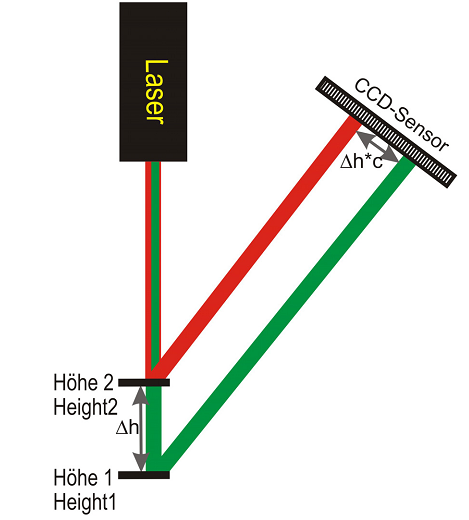
\includegraphics[scale=1.5]{bilder/lasertriangulation}
	\caption[Prinzip der Lasertriangulation]{Prinzip der Lasertriangulation mit $\Delta h:$ Objekthöhe, c: Triangulationsfaktor \protect\footnotemark}
\end{figure}
\footnotetext{Quelle: \cite{gindorf}}

Zusätzlich muss die thermische Ausdehnung erfasst und am Messobjekt kompensiert werden, da hier durch das Beschichten Temperaturerhöhungen von bis zu $150^\circ\text{C}$ entstehen können. Dies würde einer Schichtdicke von $400 \mu m$ entsprechen. Um die Genauigkeit zu steigern, erfolgt die Erfassung der Temperatur durch einen im Bauteil verarbeiteten Messsensor, der die Kerntemperatur des Messobjektes und nicht die nur wenig aussagende Oberflächentemperatur liefert. Zu beachten ist eine, durch das Material bedingte, verzögerte Erfassung der tatsächlichen Temperatur, was auf die Wärmeleitfähigkeit des Materials zurückzuführen ist \cite{gindorf}. 
\\

Die Genauigkeit der Bauteile ist im Flugzeugbau, sowie in allen anderen Branchen, abhängig von der Positionierung und Genauigkeit der Montagevorrichtung und Maschinen. Deren Genauigkeit wiederum ist abhängig von den Messgeräten und von der Vorgehensweise bei ihrer Ausrichtung und Positionierung. \\
Da im Flugzeugbau häufig Montagevorrichtungen in der Größenordnung von 12m vorzufinden sind, werden häufig Lasertracker zur Ausrichtung und Justage verwendet \cite{Muelaner2011}.\\
Bei der Überwachung der Montagevorrichtung ist es notwendig die thermischen Effekte zu kompensieren, da andernfalls für einige Spannvorrichtungen, nur durch die Ausdehnung, die Toleranzen überschritten werden. Ebenso existiert hier das Problem, dass die Montagevorrichtungen und Spannvorrichtungen aus anderen Materialien gefertigt wurden, als die Bauteile selbst, sodass hier unterschiedliche Ausdehnungen vorzufinden sind. Ein Ansatz von \cite{Muelaner2011} ist an diesen Stellen einheitliche Materialien bei der Vorrichtung, sowie beim Bauteil, zu verwenden.\\
Um die Ausdehnung der Vorrichtung zu erfassen ist in \cite{Muelaner2011} der Ansatz von \glqq Multilateration\grqq zu finden. Dies bedeutet, dass ein Netzwerk von Interferometern an der Montagevorrichtung angebracht wird, das diverse Streckenkombinationen, die die Montagevorrichtung bestmöglich abdecken, überwacht. Somit lässt sich eine Ausdehnung des Objektes erfassen, ohne dessen Temperatur und Material kennen zu müssen \cite{Muelaner2011}.\\
Die Kompensation erfolgt in der Annahme einer linearen thermischen Ausdehnung, was zu großen rechteckigen Strukturen passt. Bei den im Flugzeugbau vorzufindenden Montagevorrichtungen handelt es sich jedoch meist um komplexe Strukturen, für die das lineare Modell nur annähernd gute Lösungen liefert \cite{Muelaner2011}.

\section{Identifikation von Deformationen mit dynamischen Strukturmodellen}\label{sec:stahlsäule}

Zur Erfassung temperaturbedingter Deformationen in der industriellen Fertigung stellt \cite{Eichhorn2005} ein auf dynamischen Strukturmodellen basierendes Verfahren mit Methoden der adaptiven KALMAN Filterung vor.\\
Da diese Modelle eine zeitliche Abfolge berücksichtigen, liefern sie realitätsnahe mathematische Modelle zum untersuchten Deformationsvorgang und bieten umfangreiche  Interpretationsmöglichkeiten \cite{Eichhorn2005}. Grundlage für die Modelle ist die Beziehung der gemessenen Oberflächentemperatur am Objekt, die als Systemeingang verwendet wird, und der resultierenden Deformation, welche der Systemausgang ist.\\
Als experimentelle Untersuchung wurde eine dünnwandige Aluminiumsäule verwendet, die einseitig, entlang eines Vertikalprofils, durch eine äußere Wärmequelle erhitzt wird. 
\newpage
\begin{figure}[h]
	\label{fig:stahlsaeule}
	\centering
		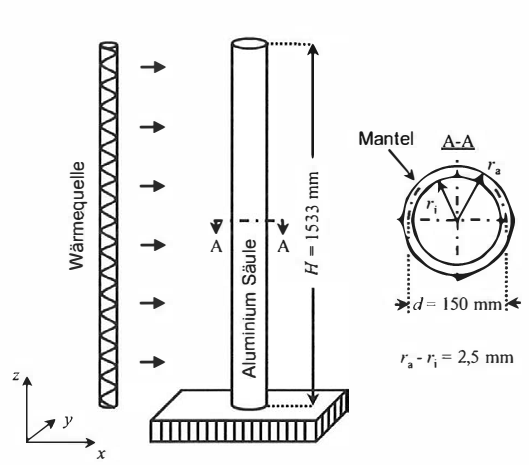
\includegraphics[scale=1.5]{bilder/erwaermungStahlsaeule}
	\caption[Einseitige thermische Belastung einer Aluminiumsäule]{Einseitige thermische Belastung einer Aluminiumsäule \protect\footnotemark}
\end{figure}
\footnotetext{Quelle: \cite{Eichhorn2005}}

Die für die Analyse notwendigen Bestimmungen der instationären Temperaturverteilung und der Leitfähigkeit, sowie Versuchsaufbau, -durchführung und die Ergebnisse des Versuches sind in \cite{Eichhorn2005} und \cite{Eichhorn2005a} genauer beschrieben und aufgeführt.\\
Die Abhängigkeit zwischen der Temperatur als Eingangsgröße auf ein Objekt und die Verformung des Objektes ist in folgender Grafik von \cite{Eichhorn2005a} dargestellt.
\begin{figure}[h]
	\label{fig:temperatureinfluss}
	\centering
		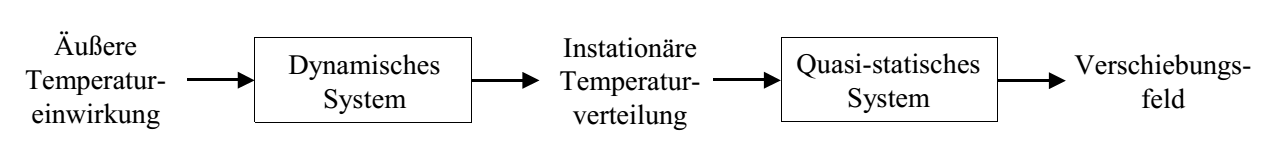
\includegraphics[scale=1.5]{bilder/temperatureinfluss}
	\caption{Verformung des Körpers durch Temperatureinfluss}
\end{figure}
Die äußere Temperatureinwirkung wirkt dynamisch auf das Objekte, was eine zeitliche Verzögerung bei der Wärmeverteilung im Inneren zur Folge hat. Die Temperatur im Inneren des Objektes hingegen wirkt sich verzögerungsfrei auf die Verformung des Messobjekts aus.

\section{Unsicherheiten}\label{sec:unsicherheiten}

Auch nach der Anwendung einer Temperaturkompensation existieren noch einige Unsicherheiten, die durch die Eingangsgrößen und Bedingungen nicht gänzlich eliminiert werden können.\\
Diverse Faktoren wirken sich auf die Messung der Temperatur aus. Einen großen Einfluss auf die Genauigkeit hat der Erfassungsort der Temperatur. Wird nur die Raumtemperatur in der direkten Umgebung des Objektes erfasst, so kann diese sich dennoch stark von der tatsächlichen Objekttemperatur unterscheiden und zu fehlerhaften Annahmen und Korrekturen der Ausdehnung führen \cite{Neumann08}. Ebenso ist es zu unterscheiden, ob die Oberflächentemperatur des Objektes erfasst wird, oder ob durch einen Sensor im Inneren des Objektes die Kerntemperatur, oder eine Temperatur sehr nahe an der Kerntemperatur, erfasst wird. In den meisten Fällen der Praxis ist es jedoch nicht möglich die Kerntemperatur des Messobjektes zu erfassen, weshalb die Kompensation mit der Oberflächentemperatur durchgeführt wird.\\
Aus diesem Grund ist es von großer Bedeutung die Oberflächentemperatur möglichst genau zu erfassen. Moderne Infrarotsensoren bieten hierzu Genauigkeiten von $\pm0.01^\circ\text{C}$\cite{Doiron2006}. Des weiteren sollten bei der Messung möglichst für das Objekt signifikante Messstellen erfasst werden, die die Objekttemperatur möglichst gut widerspiegeln und Einfluss auf die Ausdehnung des Objektes haben \cite{Fletcher2005}. Dies kann durch das Messen der Temperatur an mehreren Stellen, oder das Erfassen der Temperatur mit mehreren Sensoren verstärkt werden.\\
Auch bei Messen in klimatisierten Räumen verbleibt eine thermisch bedingte Restunsicherheit \cite{Neumann08}.
Neben der Erfassung der Temperatur spielt auch die Angabe des Ausdehnungskoeffizienten eine Rolle. Die Angaben der Koeffizienten können in einigen Fällen um bis zu 10\% vom tatsächlichen Ausdehnungskoeffizient des Werkstückes abweichen. Auch sind in einigen Fällen Inhomogenitäten in den Koeffizienten der Werkstücke vorzufinden, die eine richtungsabhängige Ausdehnung zur Folge haben. Das Verwenden und Kombinieren verschiedener Materialien in einem Werkstück spiegelt sich in der Abweichung des Ausdehnungskoeffizienten ebenso wieder \cite{Bryan1965}. Form, Maße und Dicke des Werkstückes haben ebenfalls Einfluss auf die Ausdehnung, da Stellen mit unterschiedlicher Dicke sich nicht homogen ausdehnen, sondern zu einer Verformung des Objektes führen können \cite{Neumann08}. \\
Eine Verbesserung zur genaueren Angabe des Ausdehnungskoeffizient könnten bessere Materialkontrollen und chemische Kontrollen der Materialzusammensetzung der Werkstücke leisten \cite{Bryan1965}.\\
In \cite{Doiron2006} ist eine Gegenüberstellung einiger eindimensionaler Testmessung an einem Maßstab unter verschiedenen kontrollierten Temperaturzuständen vorzufinden, mit dem Fazit, dass thermisch kontrollierte Umgebungen am besten für Präzisionsmessungen geeignet sind, dies jedoch in der Praxis nur bedingt umsetzbar ist.\\
Wie in \cite{Bryan1965} beschrieben, ist es jedoch mindestens genau so erforderlich die zeitliche Veränderung der Temperatur zu erfassen und bei der Kompensation zu berücksichtigen, da die zeitliche Variation der Temperatur stark mit der Messgenauigkeit korreliert.\\
Die Methode zur Erfassung der Ausdehnung über Streckenmessungen, hat gegenüber des anderen Verfahrens den Vorteil, dass keine Temperaturerfassung des Messobjektes und keine Angabe des Ausdehnungskoeffizienten erforderlich ist, sodass die Unsicherheit in deren Angabe keinen Einfluss auf das Ergebnis hat. Die Unsicherheit bei dieser Variante hängt von der Messgenauigkeit des Messgerätes, der Kalibrierung und der Messanordnung ab. Weiterer Faktor ist die Anzielgenauigkeit und die Stabilität und Genauigkeit der Referenzpunkte.

\section{Zusammenfassung und Beurteilung}\label{sec:beurteilung}

Die in den Kapitel \ref{sec:teleskop} bis \ref{sec:stahlsäule} aufgeführten Verfahren der Temperaturkompensation weisen verschiedene Vorgehensweisen zur Bestimmung der Ausgangsgrößen und zur Verarbeitung dieser auf. Anhand der vorgestellten Methoden sollen nun Vor- und Nachteile erarbeitet werden, die für die spätere Umsetzung und Implementierung des zu erstellenden Verfahrens berücksichtigt werden.\\
Ziel des Verfahrens soll die Anwendung im Bereich der mobilen Messtechnik sein, was zu einigen Einschränkungen bei der Wahl der Methodik zur Bestimmung der thermischen Deformation führt. Die in Kapitel \ref{sec:flugzeugbau} vorgestellte Methode zur Erfassung der Ausdehnung über Interferometrie ist vorteilhaft, da hier die Ausdehnung nur durch das Messgerät erfasst wird. Es ist keine Erfassung der Temperatur und des Ausdehnungskoeffizienten nötig. Dies könnte, wie in Kapitel \ref{sec:unsicherheiten} genauer beschrieben, zu verbleibenden Restunsicherheiten führen. Um die Komplexität zu verringern könnte die Ausdehnung auch mit nur einem Lasertracker bestimmt werden, in dem bestimmte Punkte erfasst und durch Transformationen zu den Sollwerten die Deformation ermittelt wird.\\
Falls ein Verfahren gewählt wird, bei dem die Temperaturerfassung notwendig ist, so sollte beachtet werden, dass diese möglichst schnell und präzise erfassbar sein soll. Das Verwenden von Infrarotkameras bietet flächenhafte Wärmebilder, führt jedoch auch zu weiteren Auswerteschritten. Die Erfassung der Objekttemperatur sollte mit Kontaktthermometer oder Infrarotsensoren erfolgen. Das Anbringen von Sensoren im Inneren des Bauteils liefert genauere Temperaturmessungen, ist jedoch in der Praxis meist nicht umsetzbar, da das Objekt nicht beschädigt werden darf.\\
Ebenso liefern Simulationen zur Bestimmung von Deformationen meist sehr genaue Ergebnisse, sind jedoch sehr schwer zu Implementieren und benötigen möglichst exakte Eingangsparameter. Diese werden häufig durch Verwenden komplexer Messanordnungen und großer Anzahl von Temperatursensoren umgesetzt. Die Folge ist eine zusätzliche Verarbeitung von vielen Eingangsdaten.\\
Die Verfahren und aktuelle kommerzielle Softwarelösungen deuten darauf hin, dass eine Kompensation der Messwerte, wie in \cite{Hernla2013} beschrieben, in Richtung des Koordinatenursprungs erfolgt. Eine konkrete Angabe des Vorgehens und der Berechnung lässt sich aus den aktuellen Veröffentlichungen nicht erarbeiten und hervorheben.

\chapter{Entwicklung des Verfahren zur Temperaturkompensation}\label{chap:entwicklung}

In diesem Kapitel soll die Theorie für das zu implementierende Verfahren näher erläutert werden. Ebenso werden die ersten Grundbausteine erläutert und die Zusammenhänge dargestellt. Zu Beginn erfolgt eine kurze Beschreibung der Open- Source- Softwarelösung OpenIndy, in welche die Funktionalitäten implementiert werden.

\section{OpenIndy}\label{sec:openindy}

OpenIndy ist eine Open-Source-Softwarelösung für den Bereich der industriellen Messtechnik. Das langfristige Ziel dieses Projektes ist die Verwendung der Software im Bereich der Forschung und Lehre, sowie in der Praxis. Die Open-Source-Software ist unter der Lesser General Public License lizensiert und in einem öffentlichen Repositorium\footnote{https://github.com/openindy/} hinterlegt. Es wurde mit dem Qt-Creator\footnote{http://qt-project.org/}, einem C++ Framework, entwickelt.\\
Die Umsetzung des Verfahrens zur Temperaturkompensation erfolgt zum einen im Hauptprogramm von OpenIndy und zum anderen im ebenso frei zugänglichen \glqq Default-PlugIn\grqq, das auch im zuvor genannten Repositorium erhältlich ist.\\
Durch das PlugIn Konzept von OpenIndy ist es so leicht möglich neue Funktionalitäten beizufügen \cite{Wambach2014}. Die für das Verfahren notwendingen Funktionen, wie Transformationen, werden im Default-PlugIn implementiert. Funktionalitäten, die die Anwendung und Logik dieser betreffen werden im Hauptprogramm von OpenIndy entwickelt.\\
Weitere Informationen und ausführliche Beschreibungen von OpenIndy und dessen Funktionalitäten sind in \cite{Wambach2014} und im Wiki auf der Homepage des Repositoriums zu finden.

\section{Grundkonzept und Movements}\label{sec:grundkonzept}

Im Rahmen der Masterarbeit werden zwei verschiedene Varianten zur Temperaturkompensation eines Messobjektes in OpenIndy implementiert, die beide auf dem selben Grundkonzept basieren.\\
Beide Varianten haben gemeinsam, dass sie eine Transformation verwenden, um den Bezug zwischen Standpunkt des Messgerätes und Objektkoordinatensystem herzustellen. Diese Transformation ist für die gesamte Messzeit gültig und wird durch zusätzlich Transformationen erweitert, die eine Änderung der Temperatur und Ausdehnung des Messobjektes kompensieren.
\begin{figure}[H]
\vspace{-0.5cm}
	\label{fig:trafoverkettung}
	\centering
		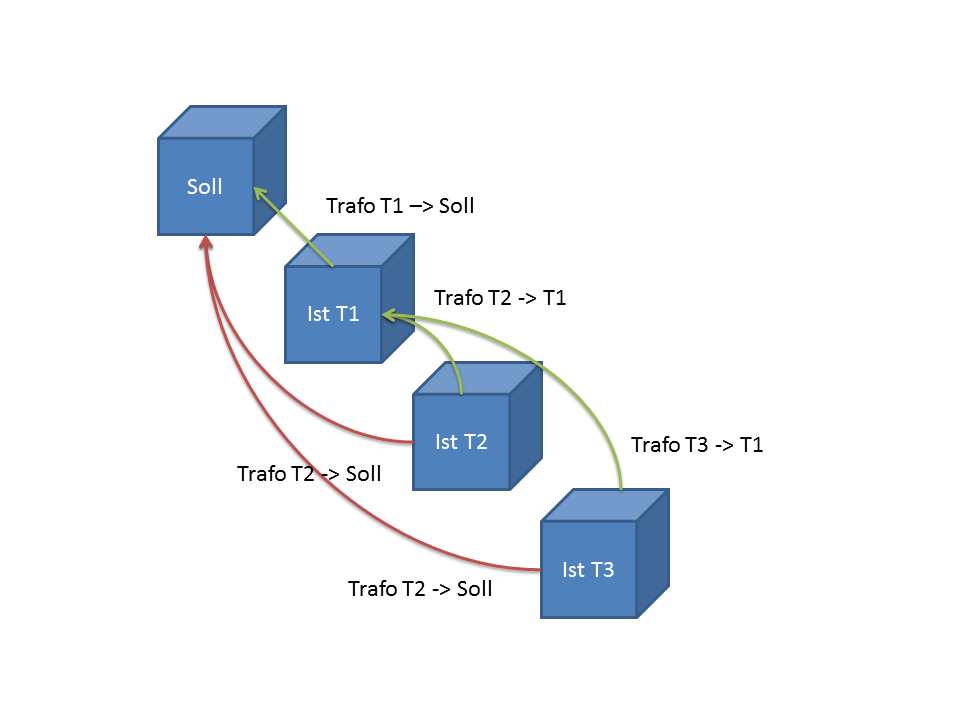
\includegraphics[scale=0.5]{bilder/transformationsverkettung}
	\caption[Anwendungslogik von Transformationen in OpenIndy]{Anwendungslogik von Transformationen in OpenIndy. grün = Umsetzung OpenIndy; rot = Alternative}
\end{figure}
Grafik \ref{fig:trafoverkettung} zeigt die Anwendungslogik von Transformationen in OpenIndy. Wie zu entnehmen ist, werden verschiedene Transformationen zur Temperaturkompensation verkettet. \\
Die Transformation, die den Bezug zum Koordinatensystem des Messobjekts herstellt, bleibt dauerhaft aktiv. Findet eine weitere Ausdehnung durch Temperaturänderung statt, so werden zusätzliche Transformationen angewandt, um den aktuellen Zustand des Messobjekts auf den Zustand der Einmessung wieder herzustellen.\\
Alternativ könnte bei jeder Temperaturänderung eine neue Einmessung in das Objektkoordinatensystem durchgeführt werden. Dieser Ansatz ist mit OpenIndy standardmäßig möglich, wird im Rahmen der Temperaturkompensation jedoch nicht weiter beachtet.\\
Bereits bei der Einmessung in das Objektkoordinatensystem im Zustand \glqq Ist T1\grqq, findet eine Kompensation der Temperatur auf den Sollzustand statt. T1 stellt hier die Ausdehnung zum Temperaturzustand bei Beginn der Messung dar. T2 und T3 stellen Änderungen in der Temperatur und Ausdehnung im Bezug zu T1 dar und werden durch Transformationen auf den Zustand T1 kompensiert. \\
Die zusätzlichen Transformationen, die meist nur aus einem Maßstab bestehen (Iststrecke/Sollstrecke aus Sollwerten), werden nach Anwendung der Transformation, die den Bezug zum Objekt herstellt, auf einzelne Beobachtungen eines Instrumentenstandpunktes (Station) angewandt, um die resultierenden Restklaffen zu kompensieren. Diese ergänzenden Transformationen werden in OpenIndy als \textbf{Movements} bezeichnet und besitzen gegenüber einer normalen Transformation einige zusätzlich zu beachtende Attribute.\\
Bei Anwendung der Movements ist darauf zu achten, auf welche Beobachtungen sie angewandt werden. Die Movements sind durch Angabe einer Zeit nur für einen bestimmten Zustand des Messobjekts gültig. Sie dürfen deshalb nur auf Beobachtungen angewandt werden, die in diesem Zeitraum erfasst wurden.\\
Der Ablauf einer Messung mit Anwendung dieser beiden Verfahren wird in den Grafiken \ref{fig:ohnemassstabSequenz} und \ref{fig:massstabSequenz} gezeigt und in den Kapiteln \ref{sec:funktionen} und \ref{chap:testmessungen} näher erläutert.

\begin{figure}[H]
	\label{fig:ohnemassstabSequenz}
	\centering
		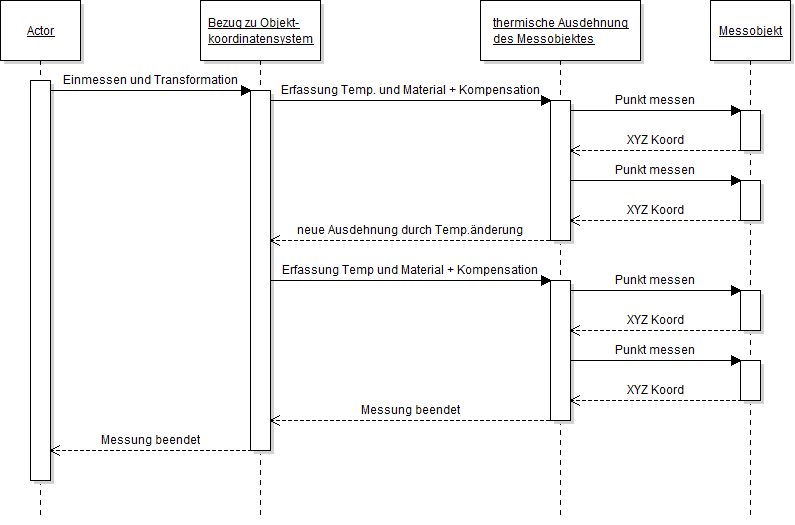
\includegraphics[scale=0.5]{UMLDiagramme/einmessen6paramSequenzUML}
	\caption[Sequenzdiagramm zur Einmessung ohne Maßstab]{Sequenzdiagramm zur Einmessung ohne Maßstab \protect\footnotemark}
\end{figure}
\footnotetext{Grafik erzeugt mit Violet UML (http://alexdp.free.fr/violetumleditor/page.php)}

Bei dieser Variante ist es erforderlich von Beginn an ein Movement anzulegen, da durch die 6 Parmater Transformation keine Reduktion der Koordinaten auf die Referenztemperatur möglich ist. Der Messablauf nach Grafik \ref{fig:massstabSequenz} ermöglicht bereits bei der Einmessung eine Korrektur auf die Referenztemperatur, und erfordert erst bei zusätzlichen Ausdehnungen durch Temperaturänderungen Movements.

\begin{figure}[H]
	\label{fig:massstabSequenz}
	\centering
		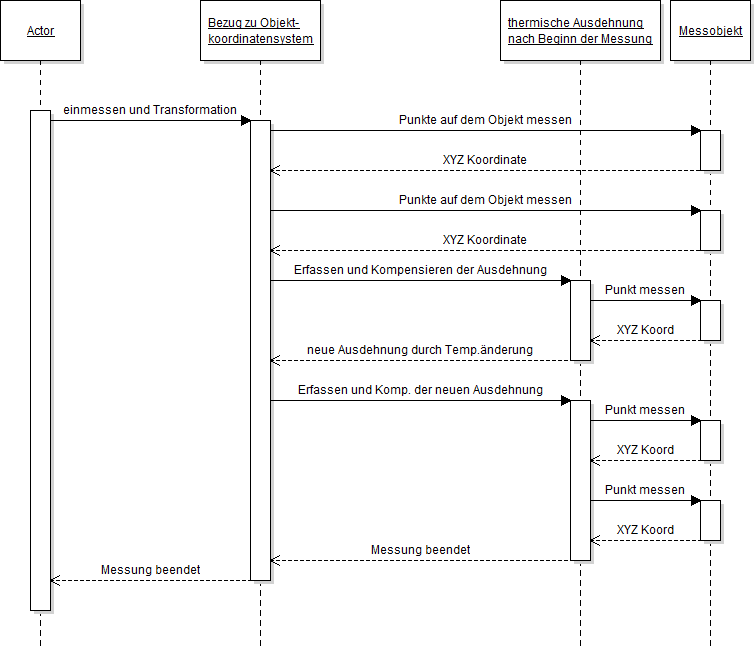
\includegraphics[scale=0.5]{UMLDiagramme/einmessenMitMassstabSequenzUML}
	\caption{Sequenzdiagramm zur Einmessung mit Maßstab}
\end{figure}

Die Anwendung der Transformationen und Movements findet über die Anwendung von homogenen Matrizen statt und soll im nachfolgenden näher erläutert werden.\\
Wird die Einmessung mit einer 6 Parameter Transformation durchgeführt, so sieht die homogene Transformationsmatrix \textbf{T}, die den Bezug zwischen Instrumentensystem und Koordinatensystem des Messobjektes herstellt, wie folgt aus.
\begin{equation}\label{eq:6paramt1}
\textbf{T}_{Station}^{Part} = \textbf{T}_{Station(TRef)}^{Part} * \textbf{T}_{Station (T1)}^{Station (TRef)}
\end{equation}
Die homogene Matrix setzt sich aus der Matrix der 6 Parameter Transformation und der Matrix zur Temperaturkompensation von T1 zur Referenztemperatur zusammen, wobei alle Matrizen homogene Matrizen sind. Ändert sich die Temperatur während der Messung, so muss die Kompensation erweitert und angepasst werden. Für den neuen Zustand gilt dann
\begin{equation}\label{eq:6paramt2}
\textbf{T}_{Station}^{Part} = \textbf{T}_{Station(TRef)}^{Part} * \textbf{T}_{Station (T2)}^{Station (TRef)}
\end{equation}
Wobei hier T2 den neuen Temperaturzustand darstellt und kompensiert.
Dieses Konzept muss bei diesem Verfahren konsequent weitergeführt werden. So würde beim Temperaturzustand Tn die Gleichung zur Kompensation wie folgt aussehen.
\begin{equation}\label{eq:6paramtn}
\textbf{T}_{Station}^{Part} = \textbf{T}_{Station(TRef)}^{Part} * \textbf{T}_{Station (Tn)}^{Station (TRef)}
\end{equation}

Wählt man zu Beginn der Messung eine Transformation mit Maßstab, um den Bezug zum Koordinatensystem des Messobjekts herzustellen, so sieht der Aufbau der homogenen Transformationsmatrix \textbf{T} wie folgt aus.
\begin{equation}\label{eq:9paramt1}
\textbf{T}_{Station}^{Part} = \textbf{T}_{Station T1}^{Part}
\end{equation}
Hier kompensiert der Maßstab der Transformation bereits die Objektausdehnung, weshalb kein Movement angewandt werden muss. Bei Veränderung der Temperatur ist es nötig ein Movement anzubringen, um die Ausdehnung zu kompensieren. Hierzu würde die homogene Matrix wie folgt aussehen.
\begin{equation}\label{eq:9paramt2}
\textbf{T}_{Station}^{Part} = \textbf{T}_{Station (T1)}^{Part} * \textbf{T}_{Station (T2)}^{Station (T1)}
\end{equation}
Die Ausdehnung zum Temperaturzustand T2 wird auf den Zustand T1 transformiert und anschließend von T1 auf die Referenztemperatur transformiert. Auch dies ist beliebig erweiterbar für weitere Temperaturänderungen und würde bei eine weiteren Temperaturänderung wie folgt aussehen.
\begin{equation}\label{eq:9paramt3}
\textbf{T}_{Station}^{Part} = \textbf{T}_{Station (T1)}^{Part} * \textbf{T}_{Station (T3)}^{Station (T1)}
\end{equation}
Die durch Temperatur T3 erzeugte Ausdehnung wird auf die Ausdehnung zu Temperatur T1 und anschließend auf TRef transformiert.\\
Betrachtet man nun die Sequenzdiagramme \ref{fig:einmessen6param} und \ref{fig:einmessenmassstab} gemeinsam mit den dazugehörigen Gleichungen \ref{eq:6paramt1} bis \ref{eq:6paramtn} und \ref{eq:9paramt1} bis \ref{eq:9paramt3}, so ist festzustellen, dass bei Wahl einer Transformation mit Maßstab um den Bezug der Koordinatensysteme herzustellen, vorerst kein Movement angewandt werden muss. Erst bei weiteren Ausdehnungen, muss die Transformationskette durch Movements erweitert werden, sodass der aktuelle Zustand des Messobjektes kompensiert werden kann. Bei Wahl der 6 Parameter Transformation muss von Beginn an mit Movements gearbeitet werden, dass die thermisch bedingte Ausdehnung kompensiert werden kann.\\

Da es sich bei der normalen Transformation, als auch bei den Movements, um die selbe Klasse handelt, ist es notwendig hier eine Variable zur Unterscheidung der beiden Transformationen einzubringen, da sich ihre Anwendung unterscheidet.\\
Ebenso muss die Möglichkeit zur Angabe des Gültigkeitsbereiches von Movements gegeben sein, da diese, wie den Grafiken \ref{fig:ohnemassstabSequenz} und \ref{fig:massstabSequenz} zu entnehmen ist, nur für einen bestimmten Zeitraum gelten und auf die Beobachtungen angewandt werden dürfen. Des weiteren soll bestimmt werden können, ob eine Transformation oder ein Movement angewandt werden soll. Auch hierfür wurde die Klasse \cClass{TrafoParam} um ein Attribut erweitert.\\
Das Startkoordinatensystem und das Zielkoordinatensystem eines Movements sind immer identisch und können nur Instrumentensysteme sein. Dies kommt dadurch zu Stande, dass bereits eine Transformation in das Objektkoordinatensystem durchgeführt wurde. Es müssen nur noch die durch thermische Ausdehnung entstandenen Restklaffen der einzelnen Beobachtungen eines Standpunktes kompensiert werden. Es werden deshalb alle Beobachtungen, die von diesem Instrumentenstandpunkt, im Zeitraum des Gültigkeitsbereichs des Movements, erfasst wurden mit diesem Movement korrigiert.

\subsection{Ausdehnung von Objekten}\label{sec:ausdehnungObjekte}

Das Objekt dehnt sich, je nach Lagerung, von einem bestimmten, meist jedoch nicht genau oder gar nicht bekannten, Punkt aus. Die Ausdehnung des Messobjektes muss auf diesen Punkt zurückgerechnet werden, da es sonst nicht möglich ist, die volle Ausdehnung zu kompensieren.\\
Ebenso ist es notwendig, dass nur Koordinaten im Objektkoordinatensystem korrigiert werden um die Anforderungen von Gleichung \ref{eq:deltaL} zu erfüllen, da die Ausdehnung des Objektes abhängig von seiner Länge ist. Diese Länge kann nur durch Koordinaten im Objektkoordinatensystem repräsentiert werden, da diese den direkten Bezug zum  Objektkoordinatensystem haben. Würde man die Koordinate im Instrumentensystem korrigieren, so wäre die Strecke abhängig von der Distanz des Instruments zum Objekt. Ebenso wird bei Verwendung von mehreren Standpunkten die Ausdehnung immer zum selben Punkt kompensiert. Bei Anwendung der Kompensation zum Instrumentenstandpunkt, würde kein einheitliches System bestehen und die Beobachtungen würden alle abhängig von ihrem Instrumentenstandpunkt und dessen Abstand zum Objekt kompensiert werden.\\
In vielen Anwendungen und Softwarelösungen wird der Punkt, von dem sich das Objekt ausdehnt, durch den Ursprung des Objektkoordinatensystems repräsentiert. Dieses Modell zur Kompensation der Ausdehnung ist auch in \cite{Hernla2013} zu finden. 
\begin{quotation}
Der  Temperatureinfluss ist dann am stärksten, wenn der Abstand vom Koordinatenursprung am größten ist und die Auswerterichtung etwa zum Koordinatenursprung zeigt.
\end{quotation}
Im nachfolgenden sollen die Probleme, die durch die Annahme dieses Modells auftreten, aufgezeigt werden.
Das Objekt, das für die nachfolgenden Beispiele verwendet wird, soll frei im Raum stehen, sodass es sich in x-, y- und positiver z-Richtung ausdehnen kann. Der Koordinatenursprung liegt in der linken unteren Ecke und ist durch eine grüne Kugel gekennzeichnet. Der Verlauf der Achsen ist dem Koordinatenkreuz in der Grafik zu entnehmen. Es gilt die Annahme, dass das Objekt eine gleichmäßig verteilte und konstante Temperatur hat und sich deshalb gleichmäßig in alle Achsrichtungen ausdehnt.

Durch die Annahme des falschen Modells, ist es nicht möglich die tatsächliche Ausdehnung auf die Referenzwerte zu kompensieren, sodass in diesem Fall Restklaffen verbleiben. Die Annahme, dass der Ausdehnungsursprung dem Koordinatenursprung entspricht, weicht in diesem Fall so stark vom wirklichen Ausdehnungsursprung ab, dass keine besseren Ergebnisse nach der Kompensation erzielt werden können. Eine Simulation einer Beispielmessung für diesen Fall ist in Kapitel \ref{chap:testmessungen} enthalten.\\

\begin{figure}[H]
	\label{fig:objektausdehnung}
	\centering
	\subfigure[Axometrische Ansicht]{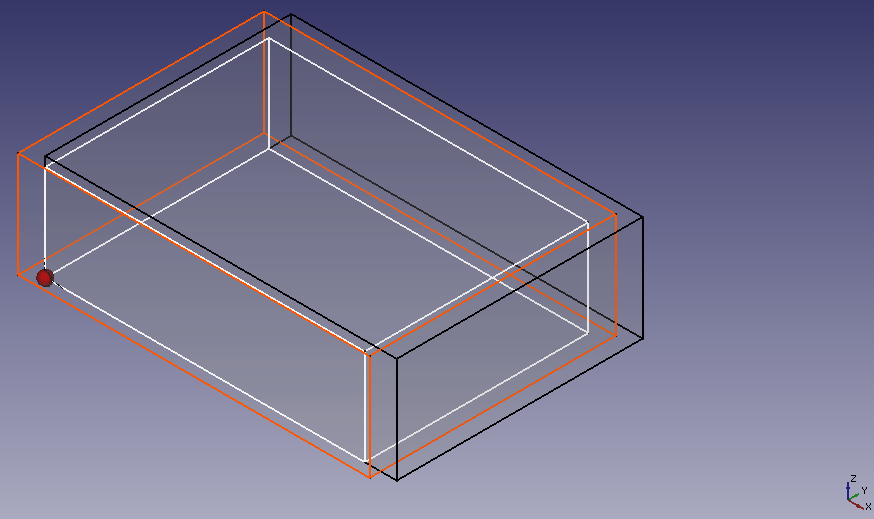
\includegraphics[width=0.49\textwidth]{FreeCADDaten/UrsprungEcke/axometrisch}}
	\subfigure[Vorderansicht]{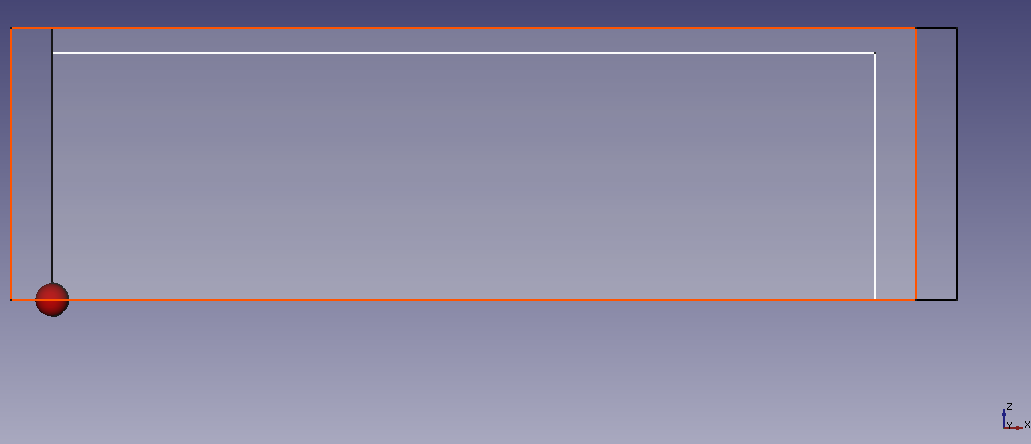
\includegraphics[width=0.49\textwidth]{FreeCADDaten/UrsprungEcke/vorderansicht}}  
	\subfigure[Oberansicht]{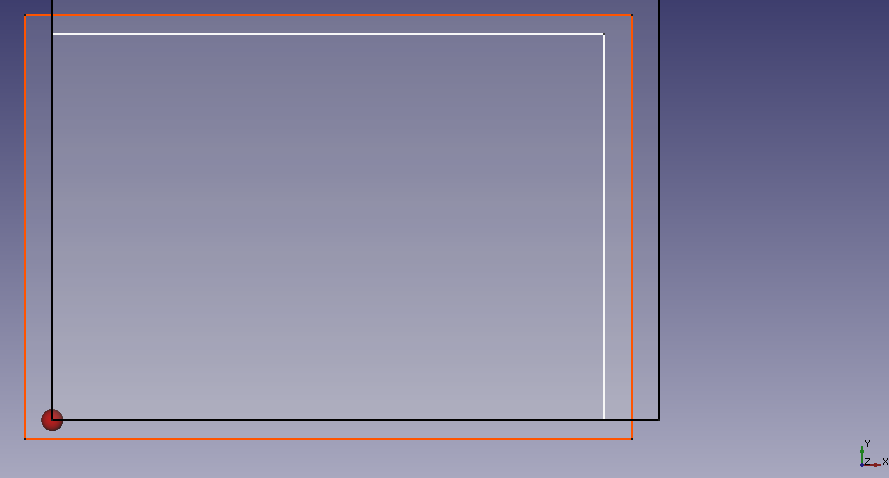
\includegraphics[width=0.49\textwidth]{FreeCADDaten/UrsprungEcke/oberansicht}} 
	\caption[Ausdehnung des Messobjekts mit Ursprung in der Ecke]{Ausdehnung des Messobjekts mit Koordinatenursprung und Ausdehnungsursprung in der Ecke. weiß = Referez schwarz = Ausdehnung nach Modell rot = tatsächliche Ausdehnung) \protect\footnotemark}
\end{figure}
\footnotetext{Grafik erzeugt mit FreeCAD (http://freecadweb.org/)}

Eine Lösung für das obige Beispiel wäre es, den Koordinatenursprung bestmöglich an den Ausdehnungsursprung anzunähern. Da es für einige Messaufgaben jedoch vorteilhafter ist, den Koordinatenursprung an eine andere Stelle des Messobjektes zu legen, so muss der Ursprung der Ausdehnung zusätzlich angegeben werden, um genauere Ergebnisse zu erlangen. Im Rahmen der Masterarbeit wurde hierzu ein Ansatz entwickelt, in dem das Koordinatensystem neben dem Koordinatenursprung noch einen zusätzlichen Punkt besitzt. Dieser entspricht dem Ausdehnungsursprung und liegt standardmäßig im Koordinatenursprung. \\
Es ist jedoch möglich ihn zu editieren und somit das Koordinatensystem um diesen Punkt zu erweitern, der für die spätere Kompensation der Messwerte verwendet wird. Wie die Darstellung in Grafik \ref{fig:koordausdehnung2ausdursprnahe} zeigt, führt bereits eine grob angenäherte Angabe des Punktes im Bezug auf den wirklichen Ausdehnungsursprung zu deutlich genaueren Ergebnissen.

\begin{figure}[H]
	\label{fig:objektausdehnungursprung}
	\centering
	\subfigure[Axometrische Ansicht]{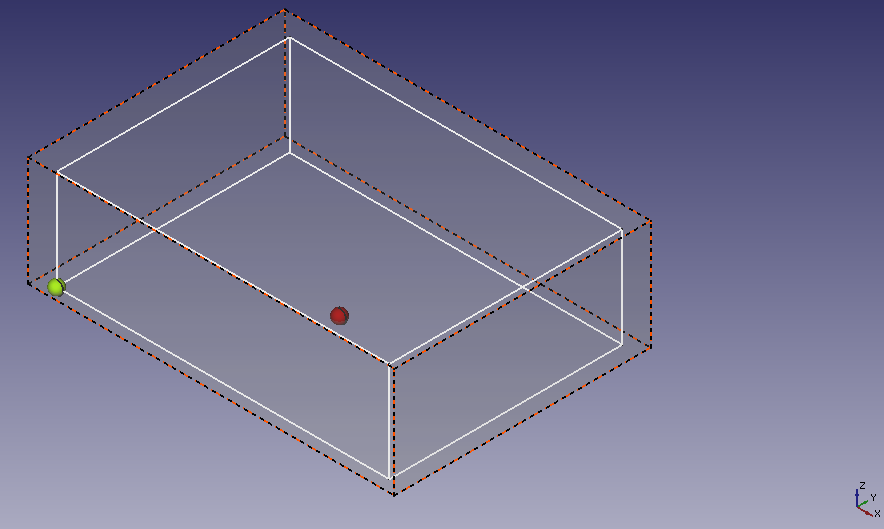
\includegraphics[width=0.49\textwidth]{FreeCADDaten/UrsprungMitte/axometrisch}}
	\subfigure[Vorderansicht]{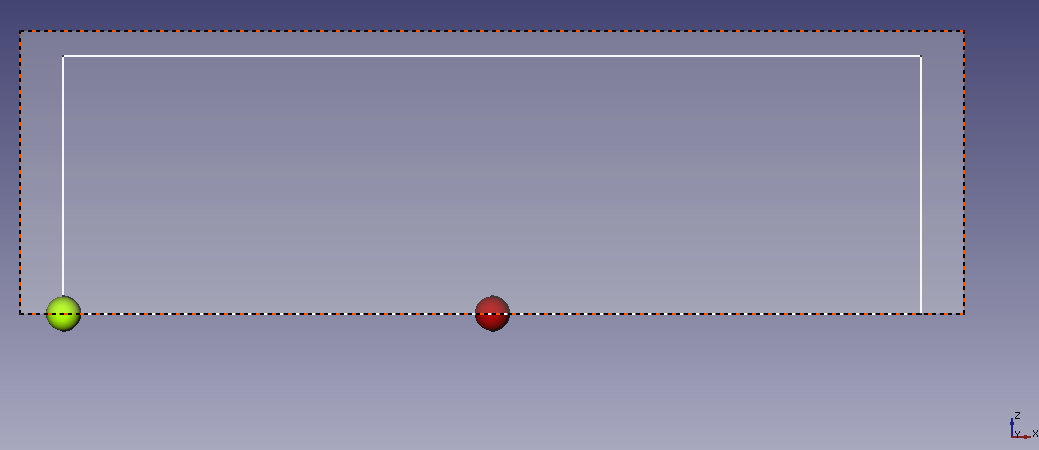
\includegraphics[width=0.49\textwidth]{FreeCADDaten/UrsprungMitte/vorderansicht}}  
	\subfigure[Oberansicht]{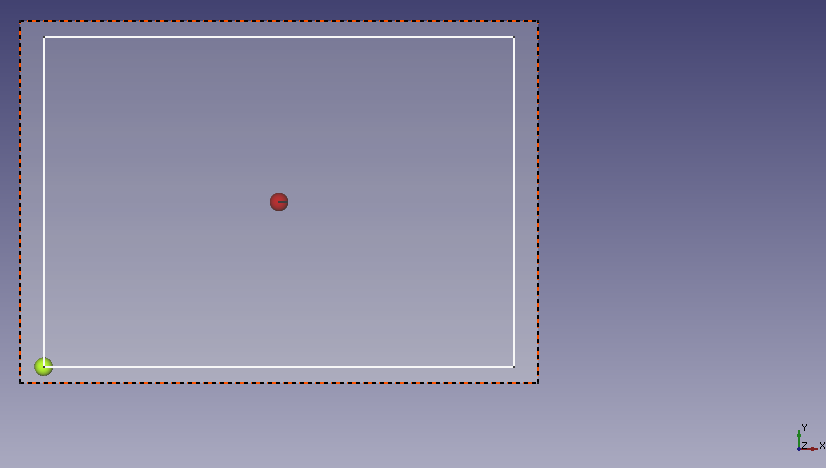
\includegraphics[width=0.49\textwidth]{FreeCADDaten/UrsprungMitte/oberansicht}} 
	\caption[Ausdehnung des Messobjekts mit Angabe von Koordinatenursprung und Ausdehnungsursprung]{Ausdehnung des Messobjekts mit Angabe von Koordinatenursprung und Ausdehnungsursprung. grüne Kugel = Koord.-Ursprung, rote Kugel = Ausdehnungsursprung,weiß = Referez schwarz = Ausdehnung nach Modell, rot = tatsächliche Ausdehnung }
\end{figure}

Wie diesen Grafiken zu entnehmen ist, entspricht die Ausdehnung aus dem Modell der tatsächlichen Ausdehnung, sodass eine genaue Kompensation der Messwerte erfolgen kann. 

\subsection{Erweiterung der Klassen Transformationsparameter und Koordinatensystem}\label{sec:klassenerweiterung}

Um die in Kapitel \ref{sec:grundkonzept} und \ref{sec:ausdehnungObjekte} genannten Anforderungen an eine Temperaturkompensation umsetzen zu können, ist es zunächst nötig die Klassen \cClass{Coordinatesystem} und \cClass{TrafoParam} zu erweitern.\\

\paragraph{\cAttr{Datumstransformation}}\label{sec:datumtrafo} wurde zusätzlich im Rahmen der Entwicklung des Verfahrens zur Temperaturkompensation in OpenIndy integriert.\\
Eine Datumstransformation ermöglicht es sich zu Beginn der Messaufgabe in das Messobjekt einzumessen und anschließend zusätzliche Verknüpfungspunkte zu erfassen, die keinen direkt Kontakt mit dem Messobjekt haben. Da das Einmessen in das Messobjekt eventuell zu komplex ist, oder wegen Sichtbarkeitsproblemen nicht von allen Standpunkten aus möglich ist, so sollte es dennoch möglich sein über die zuvor platzierten Verknüpfungspunkte eine Verknüpfung zum ersten Standpunkt herzustellen, und über dessen Transformationsparameter einen Bezug zum Messobjekt herzustellen.\\
Da das Ganze in OpenIndy automatisch ablaufen soll, durchsucht jeder Standpunkt, der keinen direkten Bezug zum Messobjekt herstellen kann, seine Liste von Transformationsparametern zu anderen Standpunkten und prüft, ob es möglich ist über diesen Standpunkt einen Bezug zum Messobjekt herzustellen. Enthält dieser Standpunkt Transformationsparameter, die als Datumstransformation markiert sind und den Bezug zum Messobjekt herstellen können, so werden die Koordinaten des aktuellen Standpunkt in das Koordinatensystem des Standpunktes mit der Datumstransformation und anschließend ins Koordinatensystem des Messobjektes transformiert.\\
Die Funktion \cFunc{OiMat getTransformationMatrix(CoordinateSystem *from)} liefert die nötige homogene Transformationsmatrix, mit der die Werte anschließend transformiert werden. Die Matrix setzt sich aus allen notwendigen Transformationsschritten zusammen, sodass sie den direkten  Bezug zum Zielsystem herstellt.
\begin{figure}[h]
	\label{fig:datumstransformation}
	\centering
		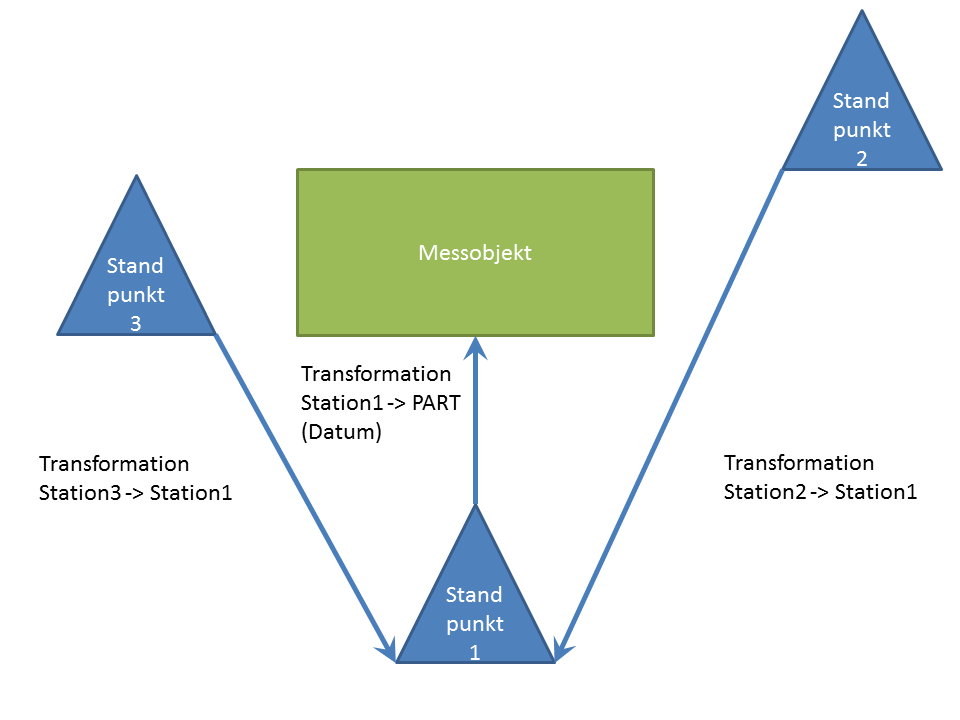
\includegraphics[scale=1.6]{bilder/datumtransformation}
	\caption{Prinzip der Datumstransformationen}
\end{figure}
\newpage  

Nachfolgend ein, zur Logik der Grafik passender, Ausschnitt aus \cFunc{OiMat getTransformationMatrix(CoordinateSystem *from)}, der die Erzeugung der Transformationskette darstellt.

\begin{lstlisting}[caption={Auszug aus \cFunc{OiMat getTransformationMatrix(CoordinateSystem *from)}},captionpos=t]

/*
*search a transformation "chain".
*watch each trafo param of the from system and check if it has a connection to another trafo param
*that has the active coord sys as start or destination system
*/

	foreach (TrafoParam *tp, from->getTransformationParameters()) {

    	if(tp->getIsUsed()){

//search trafo param in tp that are in relation to the target system
        	foreach (TrafoParam *t, tp->getStartSystem()->getTransformationParameters()) {
               //watch if the trafo param is active and can  be used in the chain
               if(t->getisDatumTrafo() && t->getIsUsed()){
                   //check if the start system is the active system
                   if(t->getStartSystem() == OiFeatureState::getActiveCoordinateSystem()){

                       OiMat tt = t->getHomogenMatrix().inv();
                       OiMat ttp;

                       if(tp->getStartSystem() == from){
                           ttp = tp->getHomogenMatrix();
                       }else{
                           ttp = tp->getHomogenMatrix().inv();
                       }

                       trafoMat = tt*ttp;

                       return trafoMat;
\end{lstlisting}

\paragraph{\cClass{TrafoParam}\protect\footnote{\url{https://github.com/OpenIndy/OpenIndy/blob/jens_masterthesis/src/trafoparam.h}}} wurde um folgende Attribute erweitert:\\
\begin{itemize}
	\item \cAttr{use} (boolsche Variable zur Festlegung, ob diese Transformation verwendet werden soll)
	\item \cAttr{validTime} (Angabe einer Uhrzeit, ab wann diese Transformation verwendet werden darf)
	\item \cAttr{isMovement} (boolsche Variable, die angibt ob es sich um eine normale Transformation oder ein Movement handelt)
	\item \cAttr{isDatumTrafo} (gibt an, ob diese Transformation vom Instrumentensystem direkt in das Objektkoordinatensystem führt und für die Verkettung mit anderen Standpunkten verwendet werden kann)
\end{itemize}

\paragraph{\cClass{CoordinateSystem}\protect\footnote{\url{https://github.com/OpenIndy/OpenIndy/blob/jens_masterthesis/src/coordinatesystem.h}}} wurde um folgende Attribute erweitert:\\
\begin{itemize}
	\item \cAttr{expansionOrigin} (ein Vektor, der den Ursprung der Ausdehnung angibt und für spätere Berechnungen verwendet wird)
\end{itemize}

Die Attribute wurden in der jeweiligen Tabellenansicht in OpenIndy hinterlegt und dargestellt. Die Standardwerte sind mit Eingabemöglichkeiten hinterlegt, sodass eine Änderung der Werte vorgenommen werden kann. Dies ermöglicht im Laufe einer Messung beispielsweise die \cAttr{validTime} eines Movements zu ändern oder Transformationen über das \cAttr{use} von der Verwendung auszuschließen. Der Ausdehnungsursprung des Koordinatensystem kann ebenfalls editiert werden. Zu beachten ist hier, dass eventuell die Transformationsparameter neu berechnet werden müssen.

\chapter{Implementierung und Umsetzung des Verfahren}\label{chap:implementierung}

Im Nachfolgenden soll das zu implementierende Verfahren genauer vorgestellt werden. Dazu wird auf das Konzept, die Funktionsweise und die Implementierung der Algorithmen und Funktionalität in OpenIndy genauer eingegangen. Die bei der Temperaturkompensation auftretenden Probleme werden mit Lösungsansätzen vorgestellt. Die Funktionalitäten sollen im Anschluss durch Beispielmessungen und simulierte Ausdehnungen eines Objektes verifiziert und validiert werden.

\section{Integration der Anwendungslogik von Transformationen und Temperaturkompensation in OpenIndy}\label{sec:anwendungslogik}

Alle für die Anwendung von Transformationen und Movements notwendigen Informationen über das Koordinatensystem, Beobachtungen, Nominalwerte und Transformationsparameter sind in der Klasse \cClass{CoordinateSystem} hinterlegt und dem jeweiligen Objekt dieser Klasse bekannt.\\
\begin{lstlisting}[caption={Ausschnitt aus coordinatesystem.h},captionpos=t]
protected:
    QList<Observation*> observations;
    QList<TrafoParam*> trafoParams;
    QList<Geometry*> nominals;

    bool isActiveCoordinateSystem;
\end{lstlisting}
In den Koordinatensystemen der Stations, also die Instrumentenkoordinatensysteme, sind alle Beobachtungen gespeichert, die von diesem Standpunkt aus erfasst wurden. Nominalwerte befinden sich in der Liste der Nominalwerte ihres zugehörigen Koordinatensystems und Transformationsparameter sind in jedem Koordinatensystem gespeichert, das als Start- oder Zielsystem aufgelistet ist.\\
Durch diese Beziehungen untereinander ist es möglich verschiedene Koordinatensysteme durch Transformationen untereinander in Bezug zu setzen und Movements auf die dazugehörigen Beobachtungen anzuwenden.

\section{Anwenden von Transformationen}\label{sec:trafoanwendung}

Alle Feature, die in einer Messaufgabe enthalten sind, werden in OpenIndy durch die statische Klasse \cClass{FeatureUpdater}\footnote{\url{https://github.com/OpenIndy/OpenIndy/blob/jens_masterthesis/controller/featureupdater.h}} verwaltet. Hierzu zählt das Erzeugen neuer Feature, das Prüfen des Featurenamen auf seine Gültigkeit, die Neuberechnung der Featureattribute und das Anwenden von Transformationen, bzw. der Aufruf  der dazugehörigen Funktionen.\\
In der Funktion \mbox{\cFunc{void switchCoordinateSystem(CoordinateSystem *to)}} wird die Liste aller Zeiger auf ein Objektkoordinatensysteme und die Liste aller Zeiger auf ein Instrumentensystem durchlaufen und deren Beobachtungen, falls welche von diesem Standpunkt aus erfasst wurden, in das Zielkoordinatensystem transformiert.\\
Zur Anwendung der Transformation und auch im späteren Verlauf der vorhandenen Movements, wurde die statische Klasse \cClass{FeatureUpdater} um ein Objekt der Klasse \\ \cClass{TrafoController}\footnote{\url{https://github.com/OpenIndy/OpenIndy/blob/jens_masterthesis/controller/trafocontroller.h}} erweitert, das für die Anwendung der Transformationsparameter auf die jeweiligen Beobachtungen zuständig ist.\\
In der zuständigen Funktion \mbox{\cFunc{bool transformObservations(CoordinateSystem *from)}} wird zunächst geprüft, ob es sich bei dem aktuell zu transformierenden Koordinatensystem bereits um das Zielsystem handelt. In diesem Fall ist keine Transformation erforderlich und alle Beobachtungen des Koordinatensystems werden auf \cAttr{isValid = true} gesetzt, sodass sie für weitere Berechnungen und Anzeigen verwendet werden.\\
Ist das aktuelle Koordinatensystem nicht das Zielsystem, so wird mit der Funktion \cFunc{OiMat getTransformationMatrix(CoordinateSystem *from)} nach einer homogenen Transformationsmatrix gesucht, die den Bezug zum Zielsystem herstellt und auch die Logik der Datumstransformation (s. Kapitel \ref{sec:datumtrafo}) berücksichtigt. Liefert diese Funktion eine ungültige Matrix, so kann kein Bezug des aktuellen Koordinatensystems zum Zielsystem hergestellt werden und die Beobachtungen werden auf \cAttr{isValid = false} gesetzt. Liefert die Funktion eine gültige Transformationsmatrix, so werden die Beobachtungen, wie in Listing \ref{lst:anwendungtrafo} zu sehen, transformiert und anschließend wird geprüft, ob ein Movement für diese Beobachtung existiert und angewandt werden soll.\\
Da Movements auch Objekte der Klasse \cClass{TrafoParam} sind, mit dem Unterschied, dass Start- und Zielsystem identisch sind, sind die Movements in der Liste von Transformationsparametern des zugehörigen Koordinatensystems enthalten. Die Transformationsparameter eines Movements werden nicht in die homogene Transformationsmatrix, die den Bezug zwischen zwei verschiedenen Koordinatensystemen herstellt, integriert. Die Funktionsweise von \cFunc{bool transformObservations(CoordinateSystem *from)} wird in folgendem Source- Code Ausschnitt dargestellt.

\begin{lstlisting}[caption={Anwendung von Transformationsparametern},captionpos=t,label=lst:anwendungtrafo]
//if trafo matrix is valid
//check if matrix is 4x4 = homogeneous matrix
if(trafoMat.getRowCount() == 4 && trafoMat.getColCount() == 4){
	//transform observations
	foreach (Observation *obs, from->getObservations()) {
	obs->myXyz = trafoMat * obs->myOriginalXyz;
	obs->myStatistic.qxx = trafoMat * obs->myOriginalStatistic.qxx;
	obs->isValid = true;
	}

	//then apply movements if active system is a part system
	//if active system is a station -> do nothing
	this->CheckToApplyMovements(from);

	return true;
\end{lstlisting}

\mbox{\cFunc{void CheckToApplyMovements(CoordinateSystem *from)}} prüft hierzu, ob es sich bei dem aktuell aktiven Koordinatensystem um ein Objektkoordinatensystem handelt, und ob das aktuell zu transformierende Koordinatensystem ein Instrumentensystem mit gespeicherten Beobachtungen ist.
Ist dies der Fall, liefert die Funktion \cFunc{QList<TrafoParam*> findMovements(CoordinateSystem *from)} eine Liste aller Movements für dieses Koordinatensystem. Sind mehrere Movements in dieser Liste enthalten, so sind sie nach ihrer Zeitangabe aufsteigend sortiert.\\
Die Funktion \cFunc{void applyMovements(QList<TrafoParam*> movements,}\cFunc{ CoordinateSystem *from)} wendet anschließend die Transformationsparameter der einzelnen Movements auf die dazugehörigen Beobachtungen an. Bei den Anwendung der Movements wird der in Kapitel \ref{sec:ausdehnungObjekte} beschriebene Ausdehnungsursprung mit in die Berechnung integriert, um die Ausdehnung auf den richtigen Ursprung zurück zu rechnen. Ein Ausschnitt der Anwendung  von Movements auf die dazugehörigen Beobachtungen ist in Listing \ref{lst:anwendungmovement} zu sehen.
\begin{lstlisting}[caption={Anwndung von Movements},captionpos=t,label=lst:anwendungmovement]
void TrafoController::applyMovements(QList<TrafoParam*> movements, CoordinateSystem *from)
{
/*
The point from which the part expands. This must not be the origin of the 
part coordinate system
If the real origin of expansion is different from the simulated one, the
correction of temperature expansion
will not be correct and cannot compensate the complete expansion.
*/
    OiVec expansionOrigin = OiFeatureState::getActiveCoordinateSystem()->
    getExpansionOrigin();
    expansionOrigin.setAt(3,1.0);

    for(int i=0; i< movements.size();i++){ 
    //iterate through all movements for this station

        for(int k=0; k<from->getObservations().size();k++){ 
        //iterate through all observations of this station

            Observation *obs = from->getObservations().at(k);

            //check if there is only one movement to apply
            if(movements.size() == 1){
                //check if you can apply the movement to the observation
                if(movements.at(0)->getValidTime() < 
                	obs->myReading->measuredAt){

                    OiMat t= movements.at(0)->getHomogenMatrix();

                    //reduce part transformed observation to expansion origin 						//and apply movement.
                    OiVec tmp = obs->myXyz - expansionOrigin;
                    tmp.setAt(3,1.0);

                    tmp = t*tmp;
                    //move back to original position
                    obs->myXyz = tmp + expansionOrigin;
                    obs->myXyz.setAt(3,1.0);
                    obs->myStatistic.qxx = t* obs->myStatistic.qxx;
\end{lstlisting}

Das Attribut \cAttr{validTime} gibt an, ab welchem Zeitpunkt dieses Movement gültig ist und verwendet werden darf. Sind mehrere Movements für ein Koordinatensystem vorhanden, so wird der Gültigkeitsbereich des ersten Movements durch die Angabe der \cAttr{validTime} des nächsten Movements begrenzt.\\
Wie \ref{lst:anwendungmovement} zu entnehmen ist, muss bei der Anwendung der Movements nur noch geprüft werden, ob der Zeitpunkt, an dem die Beobachtung erfasst wurde, im Gültigkeitsbereich des Movements liegt oder nicht.\\
Ist nur ein Movement vorhanden so reicht es zu prüfen, ob die Beobachtung vorher erfasst wurde, oder im Zeitraum des Movements. Wurde sie zuvor erfasst, so wird das Movement auf diese Beobachtung nicht angewandt.
Existieren mehrere Movements, so muss geprüft werden, welches Movement auf die Beobachtung angewandt werden darf. Hierzu werden alle Movements nach ihrer \cAttr{validTime} durchsucht und das Movement mit der aktuellsten \cAttr{validTime}, die jedoch vor der Erfassungszeit der Beobachtung liegen muss, wird auf die Beobachtung angewandt.

\begin{lstlisting}[caption={Anwendung mehrerer Movements},captionpos=t]
//check if you can apply the movement to the observation
                if(movements.at(i)->getValidTime() < obs->myReading->measuredAt){
                    //check if next movement is not valid for this observation
                    if((i+1)<movements.size() && movements.at(i+1)->getValidTime() > obs->myReading->measuredAt){
\end{lstlisting}

\section{Funktionen zur Bestimmung der Ausdehnung}\label{sec:funktionen}

Ziel ist es in OpenIndy mehrere verschiedene Herangehensweisen zu implementieren, um die thermisch bedingte Ausdehnung des Objektes zu kompensieren. Um dies zu ermöglichen, wurden im Default-PlugIn mehrere Funktionen implementiert. Die Funktionen ermöglichen ein Einmessen in das Objektkoordinatensystem ohne Maßstab, mit anschließender Temperaturkompensation durch Bestimmung der Objekttemperatur und des Materials. Als Alternative ist es möglich bereits bei der Einmessung eine Transformation mit Maßstab zu wählen, sodass eine Transformation auf den Zustand des Objektes bei dessen Referenztemperatur ermöglicht wird. Anschließend kann über zusätzlich angebrachte Referenzpunkte, die zu Beginn der Messung und bei jeder Änderung der Temperatur gemessen werden, eine weitere Transformation berechnet werden, um den Zustand wiederherzustellen, der bei Beginn der Messung herrschte.\\
Die Funktionen und Kombinationsmöglichkeiten werden im nachfolgenden genauer erläutert.
\begin{figure}[h]
	\label{fig:objektausdehnung}
	\centering
	\subfigure[Axometrische Ansicht]{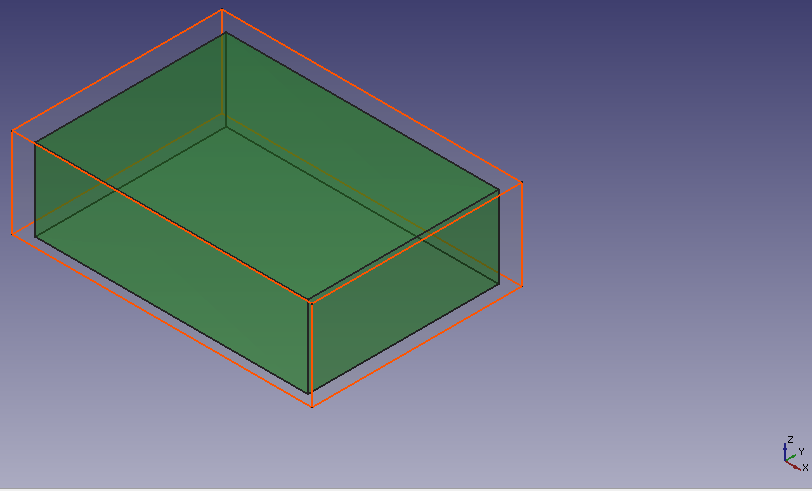
\includegraphics[width=0.49\textwidth]{FreeCADDaten/objektausdehnung}}
	\subfigure[Vorderansicht]{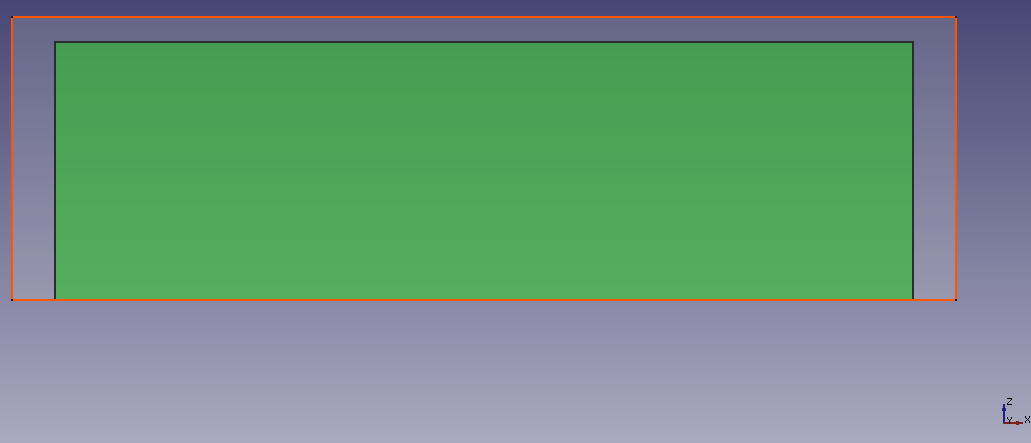
\includegraphics[width=0.49\textwidth]{FreeCADDaten/objektausdehnung2}}  
	\caption[Ausdehnung des Messobjekts]{Ausdehnung des Messobjekts grün = Referez rot = ausgedehnter Zustand) \protect\footnotemark}
\end{figure}
\footnotetext{Grafik erzeugt mit FreeCAD (http://freecadweb.org/)}

Die zuvor kurz zusammengefassten Verfahren sollen nun mit Hilfe von Use- Case-  Diagrammen näher erläutert werden. Für die Beispiele kann das Objekt aus Grafik \ref{fig:objektausdehnung} genutzt werden, für das 6 Sollkoordinaten vorhanden sind. Die Sollkoordinaten befinden sich auf der Oberseite des Objektes und sind vermarkt, sodass sie direkt messbar sind.\\

\paragraph{Variante 1} verwendet eine 6 Parameter Helmert Transformation, um den Bezug zum Objektkoordinatensystem herzustellen. Voraussetzung hierfür ist das Messen der 6 Referenzpunkte und das Einladen der Sollwerte. Die 6 Parameter Helmert Transformation wurde im Rahmen der Masterarbeit in des Default-PlugIn integriert und wird in Kapitel \ref{sec:6paramhelmert} näher beschrieben.\\
Vor Berechnung der 6 Parameter Transformation ist ein Movement mit der in Kapitel \ref{sec:standardtempcomp} beschriebenen Funktion anzulegen, der bereits in die 6 Parameter Transformation mit integriert wird, sodass deren Translationen nicht durch die thermische Ausdehnung verfälscht werden.
Nach der Transformation ist der Bezug zum Objektkoordinatensystem hergestellt, jedoch ist das Objekt noch nicht auf den Zustand zu seiner Referenztemperatur kompensiert. Aus diesem Grund werden nun die vorhandenen Movements auf die Beobachtungen angewandt.

\begin{figure}[H]
	\label{fig:einmessen6param}
	\centering
		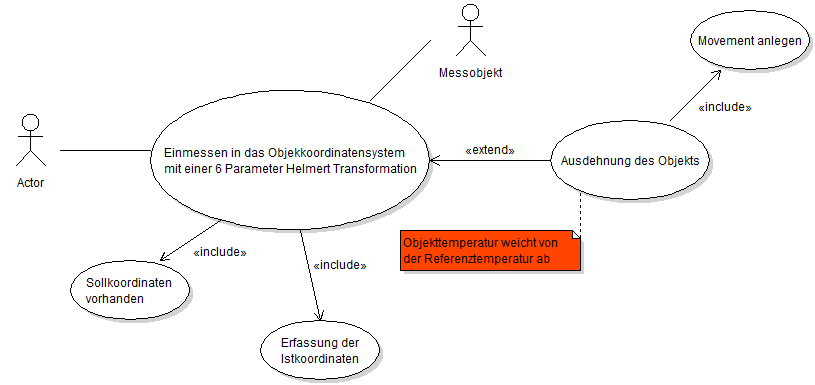
\includegraphics[scale=0.5]{UMLDiagramme/einmessen6paramUML}
	\caption{6 Parameter-Transformation in das Objektkoordinatensystem}
\end{figure}

Grafik \ref{fig:einmessen6param} zeigt noch einmal das Vorgehen, sowie Abhängigkeiten und Voraussetzungen, beim Einmessen mit einer 6 Parameter-Helmert-Transformation in Form eines Use-Case-Diagramms.

\begin{figure}[h]
	\label{fig:ausdehnungtemperatur}
	\centering
		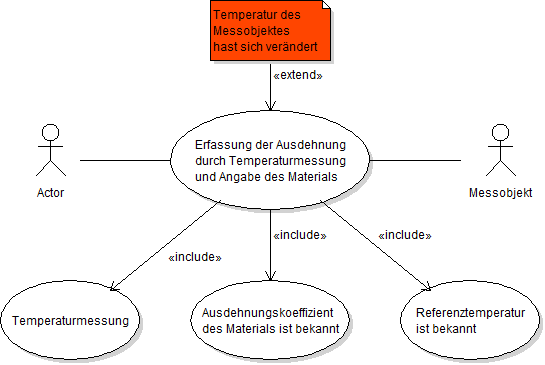
\includegraphics[scale=0.5]{UMLDiagramme/erfassungAusdehnungTemperaturUML}
	\caption{Erfassung der Objektausdehnung druch Temperaturmessung}
\end{figure}

Das Vorgehen zur Erfassung der Temperatur und der Objektausdehnung wird mit in dem Use- Case- Diagramm \ref{fig:ausdehnungtemperatur} näher erläutert und ein Ablauf einer Messung nach dieser Variante ist dem Sequenzdiagramm \ref{fig:ohnemassstabSequenz} zu entnehmen.

\paragraph{Variante 2} verfolgt das Prinzip, dass bereits bei der Einmessung in das Objektkoordinatensystem eine Transformation mit Maßstab verwendet wird. Hierzu stehen eine 7 Parameter Helmert Transformation und eine 9 Parameter Helmert Transformation, die in Kapitel \ref{sec:9paramhelmert} erläutert wird und eine Bestimmung unterschiedlicher Ausdehnungen in x- y und z- Richtung ermöglicht, zur Verfügung.\\
Direkt nach der Einmessung sollten zusätzliche Referenzpunkte am Objekt angebracht und gemessen werden. Für alle Messungen ist keine weitere Kompensation nötig, bis sich das Messobjekt aufgrund einer Temperaturänderung verformt. In diesem Fall ist ein Movement zu bestimmen. Dies wird durch erneutes messen der am Objekt angebrachten Referenzpunkte und Transformation auf den Stand der ersten Messung durch eine 7 oder 9 Parameter Transformation gelöst.  
\begin{figure}[h]
	\label{fig:einmessenmassstab}
	\centering
		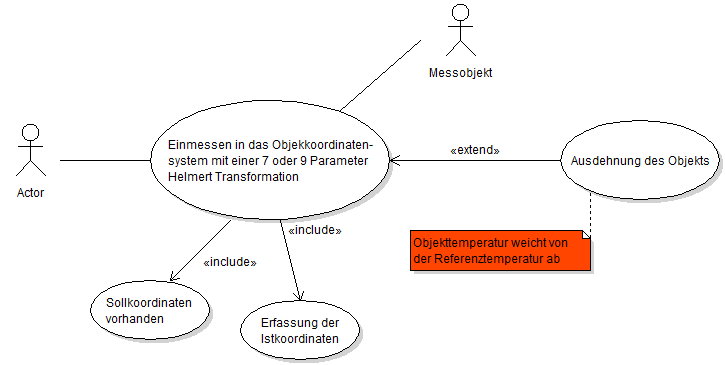
\includegraphics[scale=0.5]{UMLDiagramme/einmessenMitMassstabUML}
	\caption{Transformation mit Maßstab in das Objektkoordinatensystem}
\end{figure}

Die Grafiken \ref{fig:einmessenmassstab} und \ref{fig:ausdehnungtransformation} sollen den Ablauf der Messung nach dieser Methode grafisch verdeutlichen. Ebenso ist hierzu das Sequenzdiagramm von Seite \pageref{fig:massstabSequenz} heranzuziehen.

\begin{figure}[h]
	\label{fig:ausdehnungtransformation}
	\centering
		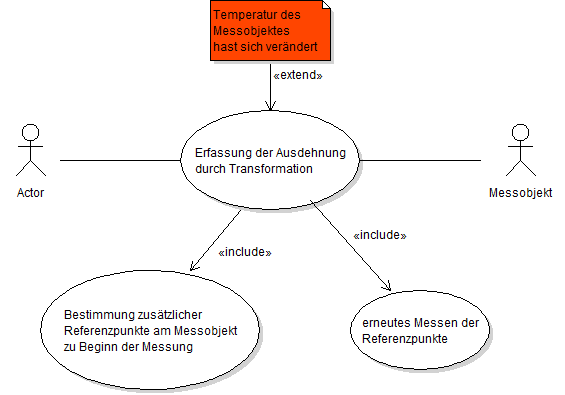
\includegraphics[scale=0.5]{UMLDiagramme/erfassungAusdehnungTransformation}
	\caption{Erfassung der Objektausdehnung durch Transformation}
\end{figure}

\subsection{Standardverfahren zur Temperaturkompensation}\label{sec:standardtempcomp}

Dieses Verfahren hat sich aufgrund der einfachen Bedienbarkeit als eines der Standardverfahren in kommerziellen Softwarelösungen durchgesetzt. Durch Eingabe der Objekttemperatur, die meist durch Messung der Oberflächentemperatur mit einem Infrarot- oder Kontaktthermometer bestimmt wird, und Festlegung des Materials des Messobjektes, lässt sich der Maßstab errechnen, der die Ausdehnung des Messobjekts darstellt. Zur Kompensation kann der Kehrwert dieses Maßstabes verwendet werden.\\
Da die Oberflächentemperatur meist nicht mit der Kerntemperatur übereinstimmt und auch der tatsächliche Ausdehnungskoeffizient sich von dem eingegebenen Wert, aufgrund von Materialabweichungen, unterscheidet (siehe Kapitel \ref{sec:unsicherheiten}), ist dieses Verfahren in seiner Genauigkeit eingeschränkt.\\
Mit Hilfe von Gleichung \ref{eq:deltaL} lässt sich der Maßstab berechnen, mit dem sich das Objekt mit der angegebenen Temperatur ausgedehnt hat. Anhand dieser Gleichung lässt sich die Ausdehnung des Werkstückes eines bestimmten Materials pro Meter und pro Grad Celcius ermitteln. Addiert man 1 zu diesem Wert, so erhält man den längen- und temperaturabhängigen Ausdehnungsmaßstab des Objektes. Der ermittelte Maßstab gilt für alle drei Koordinatenkomponenten, und ist somit nicht zur Verwendung geeignet, wenn sich das Messobjekt in den Koordinatenachsen unterschiedlich ausdehnt.
\begin{lstlisting}[caption={Bestimmung der Ausdehnung anhand von Temperatur und Material},captionpos=t]
double expansion = (actTemp-refTemp)*expansionCoefficient;
double m = 1.0/(1+ (expansion));
\end{lstlisting}
Die Eingabe der erforderlichen Werte erfolgt über ein grafisches Fenster in OpenIndy, das bei Zuweisung der Funktion zu einem Transformationsparameter erscheint. Die Angabe der Messgenauigkeit der Temperatur soll eine grobe Genauigkeitsabschätzung erlauben, da die Berechnung des Maßstabes von der Genauigkeit der Temperaturmessung abhängt. Der Ausdehnungskoeffizient wird als fehlerfrei angenommen.
\begin{figure}[H]
	\label{fig:standardverfahren}
	\centering
		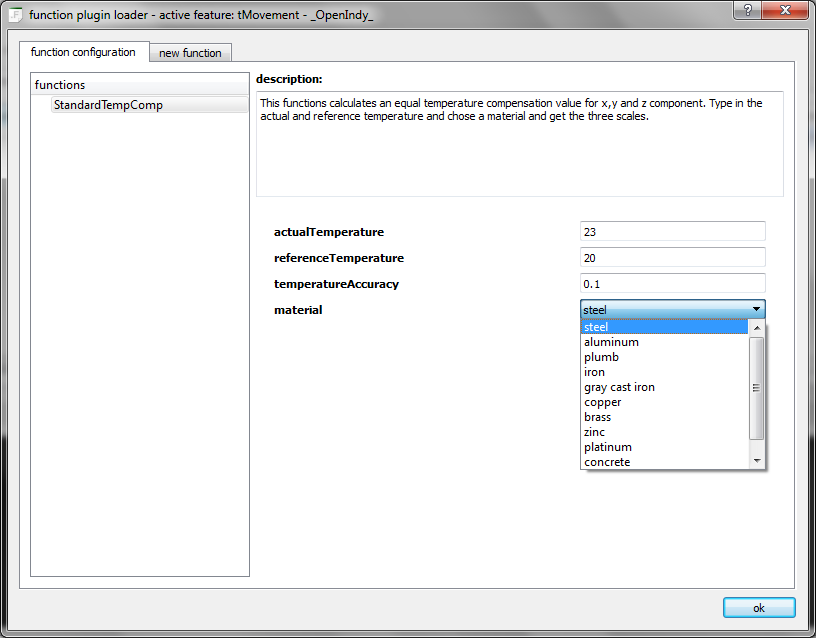
\includegraphics[scale=2.0]{bilder/standardverfahren}
	\caption[Eingabe der Parameter des Standardverfahrens]{Eingabe der Parameter des Standardverfahrens zur Temperaturkompensation}
\end{figure}

Die Liste der unterstützen Materialien ist im PlugIn hinterlegt und durch den Entwickler beliebig erweiterbar. Hierzu erfordert es nur der Angabe neuer Materialien mit ihrem Ausdehnungskoeffizient.
\begin{lstlisting}[caption={unterstütze Materialien (Ausschnitt aus \cClass{materials.h})},captionpos=t]
class Materials
{

public:
    Materials();

    enum supportedMaterials{
        eSteel,
        eAluminum,
        ePlumb,
        eIron,
        eGrayCastIron,
        eCopper,
        eBrass,
        eZinc,
        ePlatinum,
        eConcrete,
        eReinforcedConcrete
    };

    static double getExpansionCoefficient(QString material);
    static double getExpansionCoefficient(Materials::supportedMaterials material);
    static QStringList getMaterials();
\end{lstlisting}


\subsection{6 Parameter Helmert Transformation}\label{sec:6paramhelmert}

Die 3D Transformation ist Grundbestandteil diverser Softwarelösungen in der Industrievermessung, da sie den Bezug zwischen im Koordinatensystem des Messgerätes gemessenen Punkten und dem Objektkoordinatensystem herstellt \cite{Drixler1993}. Da durch die thermische Ausdehnung von Objekten sich deren Größe und Ausdehnung ändert, jedoch die Streckenverhältnisse, Winkel und die Form des Objektes gleich bleibt, ist die Helmert Transformation die am meisten benutze Transformation in diesem Aufgabenbereich. Nach Anwendung der Transformationsparameter, die je nach Variante der Helmert Transformation aus 3 Translationen, 3 Rotationen und keinem, einem oder drei Maßstäben besteht, bleibt die Form der Objekte im Zielsystem erhalten \cite{Carosio2006}.\\
Eine verbreitete Variante in der Industrievermessung ist es, über eine 6 Parameter- Transformation den Bezug zum Messobjekt herzustellen und anschließend die Ausdehnung des Messobjektes mit dem in Kapitel \ref{sec:standardtempcomp} beschriebenen Verfahren, durch Anwendung eines Maßstabes, zu kompensieren.\\
Die im Default- PlugIn entwickelte 6 Parameter Helmert Transformation wurde in der Klasse \cClass{Helmert6Param} entwickelt und arbeitet nach folgendem Verfahren.
Der funktionale Zusammenhang der 6 Parameter Transformation ergibt sich wie in \cite{Niemeier2008}, jedoch ohne Maßstab, sodass sich folgende Gleichung ergibt:

\begin{equation}
\begin{bmatrix} X \\ Y \\ Z \end{bmatrix} = \begin{bmatrix} X_{0} \\ Y_{0} \\ Z_{0} \end{bmatrix} + \textbf{R}(\omega,\phi,\kappa) * \begin{bmatrix} x \\ y \\ z \end{bmatrix}
\end{equation}

Der Ablauf zur Bestimmung der Parameter besteht aus Anwendung eines Movements, um den Einfluss der thermischen Ausdehnung auf das Objekt zu korrigieren, sodass die Berechnung der Transformationsparameter nicht beeinflusst werden.
Im Anschluss werden die Rotation und die Translation berechnet.
\newpage
\begin{lstlisting}[caption={Ausschnitt aus der \cFunc{exec} Methode},captionpos=t]
bool Helmert6Param::exec(TrafoParam &tp)
{
   this->svdError = false;
   //check wether all parameters for calculation are available
   if(this->isValid()){ 
   		//fills the locSystem and refSystem vectors based on the given common points.
        this->init(); 
        if(locSystem.count() == refSystem.count() && locSystem.count() > 1){ 			//if enough common points available

            //apply movement if necessary
            this->applyMovements(tp);

            //get rotation and translation
            this->rotation = this->approxRotation();
            this->translation =  this->approxTranslation(this->rotation);

            if(locSystem.count() > 2){

            //adjust rotation and translation if more than 2 points are available
                return this->adjust(tp);

            }else if(locSystem.count() == 3){
\end{lstlisting}

Da die Ausdehnung des Objektes durch späteres Anwenden von Movements korrigiert wird, dürfen die 6 Parameter der Transformation nicht von der Ausdehnung beeinflusst werden, da ansonsten eine doppelte Kompensation erfolgt, und die Messwerte verfälscht werden. Aus diesem Grund werden die Nominalwerte der für die Transformation verwendeten Punkte auf den Zustand der ausgedehnten Ist-Werte erweitert. Im Anschluss erfolgt die Berechnung der Transformationsparameter.

\begin{lstlisting}[caption={\cFunc{void applyMovements(TrafoParam \&tp)}},captionpos=t]

        if(t != NULL){
            
            //expand nominals with inverse of movement parameters
            for(int i=0; i<this->refSystem.size();i++){
                OiVec refP = this->refSystem.at(i);

                refP = refP - expansionOrigin;
                refP = t->getHomogenMatrix().inv()*refP;
                refP = refP + expansionOrigin;
                refP.setAt(3,1.0);

                this->refSystem.replace(i,refP);
            }
            this->protocol.append("reference points were expanded with inverse of");
            this->protocol.append(" movement transformation to get correct translation values.");
        }
\end{lstlisting}

Da die Messwerte zu diesem Zeitpunkt nur im Instrumentensystem vorliegen, ist es nicht möglich diese zu kompensieren, da eine Kompensation nur im Koordinatensystem des Messobjektes stattfinden kann. Aus diesem Grund werden die Nominalwerte mit der Inversen des Maßstabes erweitert, um die selbe Ausdehnung, wie die Ist-Werte, aufzuweisen.\\

Zur Bestimmung der Rotationswinkel wird das Verfahren nach \cite{Drixler1993} angewandt, das eine Lösung über Quaternionen vorgibt. Dies ermöglicht eine Lösung der Parameter ohne iteratives Vorgehen und ohne Bestimmen von Startwerten.
\begin{lstlisting}[caption={Berechnung der Rotationswinkel},captionpos=t]
OiVec Helmert6Param::approxRotation()
{
	//centroid coordinates
    vector<OiVec> centroidCoords = this->calcCentroidCoord(); 
        if(centroidCoords.size() == 2){
			//centroid reduced destination coordinates            
            vector<OiVec> locC = this->centroidReducedCoord(locSystem, centroidCoords.at(0)); 
			//centroid reduced target coordinates            
            vector<OiVec> refC = this->centroidReducedCoord(refSystem, centroidCoords.at(1)); 
 			//vector of model matrices - one for each common point
            vector<OiMat> modelMatrices = this->modelMatrix(locC, refC); 
			//calculate the normal equation matrix            
            OiMat n = this->normalEquationMatrix(modelMatrices); 
            OiVec q = this->quaternion(n);
            if( !svdError ){
                OiMat r = this->rotationMatrix(q); //fill rotation matrix
                OiVec result = this->getRotationAngles(r);
                
\end{lstlisting}

Zur Bestimmung der Translation wird der Schwerpunkt des Start- und des Zielsystems berechnet und voneinander subtrahiert.\\

Da in diesem Ansatz zu Bestimmung der Transformationsparameter keine Genauigkeiten bezüglich der Punkte mit integriert sind, lässt sich das Vorgehen durch ein Gauß- Helmert- Modell erweitern. Wie in \cite{Drixler1993} vorgeschlagen, werden die Punkte aus dem Ausgangssystem hierzu mit den aus der Eigenwertbestimmung ermittelten Transformationsparametern vortransformiert. Da durch dieses Vorgehen die Restklaffen sehr gering sind, ist es im weiteren Verlauf möglich mit der vereinfachten Rotationsmatrix für kleine Winkel zu arbeiten.
\begin{lstlisting}[caption={Ausschnitte aus bool adjust(TrafoParam \&tp)},captionpos=t]
bool Helmert6Param::adjust(TrafoParam &tp)
{
    //adjust trafo param if enough points are given
    bool result = false;

    //transform loc (start system) to "pseudo"-loc system
    //transformation with previosly approximated translation and rotation
    this->preliminaryTransformation();

    //get standard deviation
    double sumVV = 0.0;

    for (int i = 0;i<this->locSystem.size();i++) {
        OiVec diffVec = this->refSystem.at(i)-this->locSystem.at(i);
        sumVV += diffVec.getAt(0)*diffVec.getAt(0);
        sumVV += diffVec.getAt(1)*diffVec.getAt(1);
        sumVV += diffVec.getAt(2)*diffVec.getAt(2);

    }

    tp.getStatistic()->stdev = sqrt(sumVV/(3.0*this->locSystem.size()-6.0));

    //get new rotation and translation between pseudo-loc system and ref system
    OiVec tmpRotation = this->approxRotation();
    OiVec tmpTranslation = this->approxTranslation(tmpRotation);
\end{lstlisting}

Nach der Ausgleichung der Zuschläge für die Transformationsparameter, werden diese zu den zuvor bestimmten Werte addiert.

\begin{lstlisting}[caption={Anwenden der Zuschläge},captionpos=t]

	//calc x
    x = qxx * c;
    x0 = x0 + x;

    OiVec v = a * x - l_diff;
    OiVec vtv = v.t() * v;
    double s0_post = sqrt(vtv.getAt(0) / (3 * this->locSystem.length() - 6));
    OiMat sxx = s0_post * s0_post * qxx;

    //set the trafo parameters with the previously calulated values and the additional values from adjustment
    OiVec scale(4);
    scale.setAt(0,1.0);
    scale.setAt(1,1.0);
    scale.setAt(2,1.0);
    scale.setAt(3,1.0);

    this->translation.setAt(0,this->translation.getAt(0)+x0.getAt(3));
    this->translation.setAt(1,this->translation.getAt(1)+x0.getAt(4));
    this->translation.setAt(2,this->translation.getAt(2)+x0.getAt(5));

    this->rotation.setAt(0,this->rotation.getAt(0)+x0.getAt(0));
    this->rotation.setAt(1,this->rotation.getAt(1)+x0.getAt(1));
    this->rotation.setAt(2,this->rotation.getAt(2)+x0.getAt(2));

    OiMat r = this->getRotationMatrix(this->rotation);
    OiMat t = this->getTranslationMatrix(this->translation);
    OiMat s = this->getScaleMatrix(scale);

    tp.setHomogenMatrix(r,t,s);

\end{lstlisting}

Die Genauigkeitsangaben liegen meist nicht vor, dennoch wurde das Verfahren in die Transformation implementiert. Als Gewichtsmatrix wird die Einheitsmatrix verwendet. Somit liefern die Ergebnisse dieser Ausgleichung keine Zuschläge auf die zuvor in der Eigenwertzerlegung bestimmten Transformationsparameter \cite{Drixler1993}. Es ist jedoch leicht möglich diese Transformation um eine Gewichtsmatrix zu erweitern.

\subsection{9 Parameter Helmert Transformation}\label{sec:9paramhelmert}

Neben der 6 Parameter Helmert Transformation und der bereits vorhandenen 7 Parameter Helmert Transformation, wurde das Default- PlugIn um eine 9 Parameter Helmert Transformation erweitert.\\
Durch Verwendung dieser Funktion, soll es möglich sein die Ausdehnung des Messobjektes in X-, Y- und Z-Richtung zu erfassen. Im Gegensatz zu der 7 Parameter Transformation ermittelt diese Funktion drei voneinander unabhängige Maßstäbe. Dadurch lässt sich die Ausdehnung besser erfassen und deuten.\\
Die Transformation ist im Default- PlugIn in der Klasse \cClass{ExtendedTemperatureCompensation} enthalten.
Der funktionale Zusammenhang dieser Transformation ergibt sich aus
\begin{equation}
\begin{bmatrix} X \\ Y \\ Z \end{bmatrix} = \begin{bmatrix} X_{0} \\ Y_{0} \\ Z_{0} \end{bmatrix} + \textbf{m} * \textbf{R}(\omega,\phi,\kappa) * \begin{bmatrix} x \\ y \\ z \end{bmatrix}
\end{equation}
Wobei \textbf{m} hier die Maßstabsmatrix darstellt, die die Maßstäbe \textbf{$m_{x}$},\textbf{$m_{y}$},\textbf{$m_{z}$} auf der Hauptdiagonalen enthält.\\
Ebenso wie bei der 6 Parameter Transformation aus Kapitel \ref{sec:6paramhelmert} erfolgt die Bestimmung der Rotationsmatrix mit Quaternionen über den Ansatz von \cite{Drixler1993}.\\
Die Bestimmung der Maßstäbe erwies sich als schwierig, da diese bestmöglich bestimmt werden müssen, da sie sonst Einfluss auf die Translationen haben. Zur Bestimmung der Maßstäbe werden die Vektoren vom ersten Punkt in der Liste zu allen anderen Punkten in Start- und Zielsystem gebildet. Nachfolgend werden alle x-, y- und z- Komponenten getrennt aufaddiert und durch die Summe der Punkte geteilt. Um Messrauschen filtern zu können, werden nur Strecken ab 5cm Länge berücksichtigt. Die Maßstäbe ergeben sich somit aus den Mittelwerten der Streckenkomponenten.

\begin{lstlisting}[caption={Bestimmung der Maßstäbe für x, y und z},captionpos=t]
for(int i=1; i<this->locSystem.size(); i++){
        //get x y and z component of vector from point 0 to i in loc system
        double sxLoc = qFabs(locSystem.at(0).getAt(0)-locSystem.at(i).getAt(0));
        double syLoc = qFabs(locSystem.at(0).getAt(1)-locSystem.at(i).getAt(1));
        double szLoc = qFabs(locSystem.at(0).getAt(2)-locSystem.at(i).getAt(2));

        //get x y and z component of vector from point 0 to i in ref system
        double sxRef = qFabs(tmpRefList.at(0).getAt(0)-tmpRefList.at(i).getAt(0));
        double syRef = qFabs(tmpRefList.at(0).getAt(1)-tmpRefList.at(i).getAt(1));
        double szRef = qFabs(tmpRefList.at(0).getAt(2)-tmpRefList.at(i).getAt(2));

        //0.050m is criteria, because of noisy measurements
        //and no representative distances.
        if(sxLoc <= 0.050 || sxRef <= 0.050){

        }else{
            sx += (sxRef/sxLoc);
            countX ++;
        }
        if(syLoc <= 0.050 || syRef <=0.050){

        }else{
            sy += (syRef/syLoc);
            countY++;
        }
        if(szLoc <= 0.050 || szRef <= 0.050){

        }else{
            sz += (szRef/szLoc);
            countZ++;
        }
    }

    //if no scale could be calculated (noisy measurements),
    //set this scale component to 1.000000
    if(sx == 0.0){
        sx = 1.0;
    }else{
        sx = sx/(double)countX;
    }

    if(sy == 0.0){
        sy = 1.0;
    }else{
        sy = sy/(double)countY;
    }

    if(sz == 0.0){
        sz = 1.0;
    }else{
        sz = sz/(double)countZ;
    }
\end{lstlisting}
Die Berechnung der Translation erfolgt analog wie in Kapitel \ref{sec:6paramhelmert}. Des weiteren wurde auch bei dieser Transformation die Erweiterung durch das Gauß- Helmert- Modell hinzugefügt und mit einer Einheitsmatrix implementiert. Somit ergibt die Ausgleichung in der aktuellen Implementierung auch hier keine Zuschläge, ist jedoch leicht erweiterbar.

\subsection{Bestimmung des Movements aus einer Transformation}

Neben der in Kapitel \ref{sec:standardtempcomp} beschriebenen Variante zur Bestimmung von Movements zur Kompensation der thermischen Ausdehnung, besteht die Möglichkeit die Parameter des Movements durch eine 7 oder 9 Parameter Transformation zu bestimmen.\\
Hierzu müssen, wie in Kapitel \ref{sec:funktionen} beschrieben, zu Beginn der Messung zusätzliche Referenzpunkte angebracht und gemessen werden. Diese müssen bei jeder weiteren Temperaturänderung erfasst werden. Anschließend lässt sich eine Transformation vom aktuellen Zustand auf den Zustand zu Beginn der Messung rechnen, der die Ausdehnung des Messobjektes kompensiert. \\
Die hierfür verwendeten Referenzpunkte müssen bestmöglich über das Messobjekt verteilt sein, um die thermische Ausdehnung erfassen und repräsentieren zu können. Nur damit ist gewährleistet, dass die Transformation zwischen aktueller und der ersten Messung auch der tatsächlichen thermischen Ausdehnung entspricht.\\
Um die Beobachtungen, die in den Referenzpunkten erfasst wurden trennen zu können, wurde die Funktion \cFunc{void fillTrafoParamFunctionMovement(SystemTransformation* function, TrafoParam *tp)} in der Klasse \cClass{FeatureUpdater} implementiert, die in der Funktion \cFunc{void recalcTrafoParam(TrafoParam *tp)} aufgerufen wird, und die Punkte zur Bestimmung der Ausdehnung der Transformation zuzuweisen.\\

Der Ist Zustand des Messobjektes wird durch die ersten Messungen in die Referenzpunkte repräsentiert. Hierzu wird eine Zeitgrenze von $\pm 3 Minuten$ um die erste Beobachtung gesetzt. 

\begin{lstlisting}[caption={Bestimmung der Referenzzeit},captionpos=t]
QDateTime startTime;

    //get smallest QDateTime from first point as reference time
    if(function->getPoints().size()>0){
        startTime = function->getPoints().at(0)->getObservations().at(0)->myReading->measuredAt;
    }else{
        return;
    }
\end{lstlisting}

Alle Punkte, die der Funktion des Movements zugewiesen wurden, werden nun mit allen Beobachtungen, die in dieser Zeitgrenze liegen, neu berechnet und der Liste des Zielsystems zugewiesen.

\begin{lstlisting}[caption={Berechnung Referenzpunkte},captionpos=t]
//edit the points and assign them to the right list.
    foreach(Point *p, function->getPoints()){

        foreach (Observation *obs, p->getObservations()) {
            //only obs that are valid in the coord system of the movement
            //and transformed obs to the coord system of the movement
            if(obs->isValid){

                if(obs->myReading->measuredAt.time() > startTime.time().addSecs(-180) && //is obs in the time span
                        obs->myReading->measuredAt.time() < startTime.time().addSecs(180)){ //for being a reference obs
                    obs->isValid = true;
                }else{
                    obs->isValid = false;
                }
            }else{
                obs->isValid = false;
            }
        }
        p->recalc(); //recalc points only with obs that are in the reference time span
        if(p->getIsSolved()){ //if point can be recalced
            Point cpyPRef(*p); //create a copy and assign to the reference list
            cpyPRef.setIsSolved(true);
            mySorter.addRefPoint(cpyPRef);
        }
\end{lstlisting}

Anschließend werden alle Beobachtungen, die im Gültigkeitsbereich des Movements liegen, zur Neuberechnung der Punkte verwendet. Dies führt dazu, dass die Punkte die aktuelle Ausdehnung des Messobjekts repräsentieren. Diese werden dann der Liste des Startsystems zugewiesen.

\begin{lstlisting}[caption={Berechnung der Punkte des Startsystems},captionpos=t]

foreach (Observation *obs, p->getObservations()) {
            if(obs->myStation->coordSys == tp->getStartSystem()){//as actual state use only obs from the current station
                if(obs->myReading->measuredAt.time() > tp->getValidTime().time().addSecs(-180) && //is obs in the time span
                        obs->myReading->measuredAt.time() < tp->getValidTime().time().addSecs(180)){ //for being a actual obs
                    obs->isValid = true;
                }else{
                    obs->isValid = false;
                }
            }else{
                obs->isValid = false;
            }
        }
        p->recalc(); //recalc points only with obs that are in the actual time span
        if(p->getIsSolved()){ //if point can be recalced
            Point cpyPStart(*p); //create a copy and assign to the actual list
            cpyPStart.setIsSolved(true);
            mySorter.addLocPoint(cpyPStart);
        }
\end{lstlisting}

Alle zur Bestimmung des Movements verwendeten Beobachtungen werden, vor Berechnung des Movements, in das Objektkoordinatensystem transformiert.\\
Das Objektkoordinatensystem muss das aktive Koordinatensystem sein, um eine korrekte Berechnung zu gewährleisten. Die Beobachtungen werden mit der Funktion \cFunc{void switchCoordinateSystemWithoutMovement(CoordinateSystem *to)} transformiert. Diese Funktion transformiert die Beobachtungen in das Objektkoordinatensystem, wendet jedoch keine Movements auf die Beobachtungen an.

\chapter{Verifizierung und Validierung}\label{chap:testmessungen}

Zur Validierung und Verifizierung der zur beschriebenen Verfahren sollen in diesem Kapitel einige Ausdehnungen eines Messobjektes simuliert und mit dem im Pseudo Tracker, der im OpenIndy Default PlugIn implementiert ist, erfasst, sowie mit Hilfe von Transformationen und Movements kompensiert werden.

\section{Einfluss des Ausdehnungsursprungs}\label{sec:einflussausdehnungsursprung}

Wie in Kapitel \ref{sec:ausdehnungObjekte} beschrieben, hat die Wahl des Bezugspunktes zur Kompensation einen großen Einfluss auf das Ergebnis. Im Nachfolgenden soll der Einfluss des zur Kompensation verwendeten Ausdehnungsursprungs demonstriert werden.\\
Hierzu wird die Messung an einem Quader mit unebener Oberfläche demonstriert, vergleichbar mit Abbildung \ref{fig:objektausdehnungursprung}. Die Sollwerte für das Messobjekt sind in Tabelle \ref{tab:sollwerteecke} enthalten. Der Koordinatenursprung liegt in der linkten unteren Ecke, der Ausdehnungsursprung mittig im Objekt mit einer Z- Komponente von 0.0mm.
\begin{figure}[H]
	\label{fig:objektursprungecke}
	\centering
		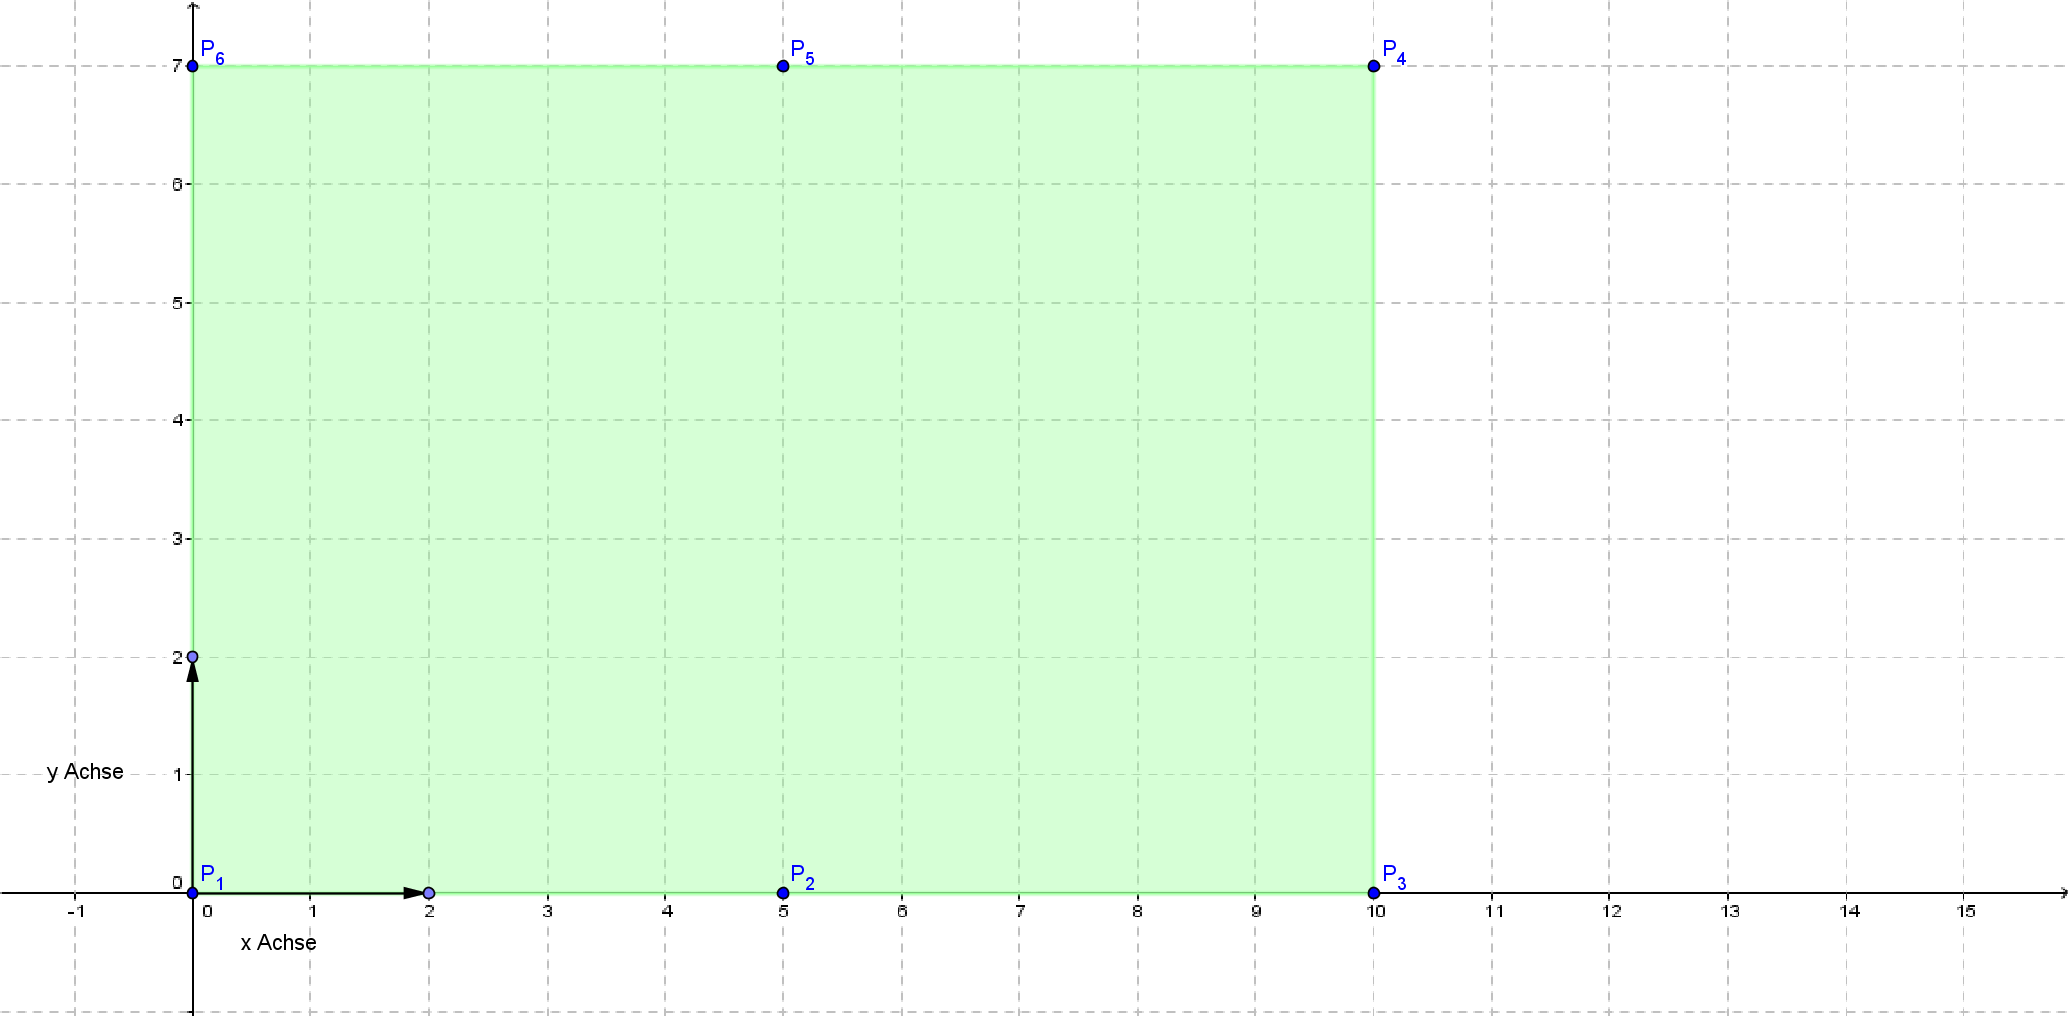
\includegraphics[scale=0.8]{bilder/objektursprungecke}
	\caption[Draufsicht auf das Messobjekt]{Draufsicht auf das Messobjekt mit Übersicht der Referenzpunkte\protect\footnotemark}
\end{figure}
\footnotetext{Grafik erstellt mit GeoGebra (http://www.geogebra.org/cms/de/)}

In einer Testmessung soll das Ergebnis demonstriert werden, bei dem Koordinatenursprung und Ausdehnungsursprung identisch sind. Die Durchführung erfolgt mit dem Pseudo Tracker und dem Messobjekt aus Grafik \ref{fig:objektursprungecke} und \ref{fig:objektausdehnung}.\\
Der Koordinatenursprung liegt in einer Ecke des Messobjektes und spiegelt nicht den tatsächlichen Punkt, von dem aus sich das Objekt ausdehnt, wider.\\
Zu Beginn der Messung ist der Pseudo Tracker als aktiver Sensor zu setzen. Hierbei ist darauf zu achten, dass im Reiter \texttt{sensor configuration} alle Instrumentenfehler auf 0 gesetzt werden, um nur den Einfluss der Ausdehnung in der Messung zu ermitteln. Andernfalls würde der Pseudo Tracker Gerätefehler simulieren und auf die Messwerte anwenden.

\begin{figure}[h]
\label{fig:sensorconfig}
\centering
	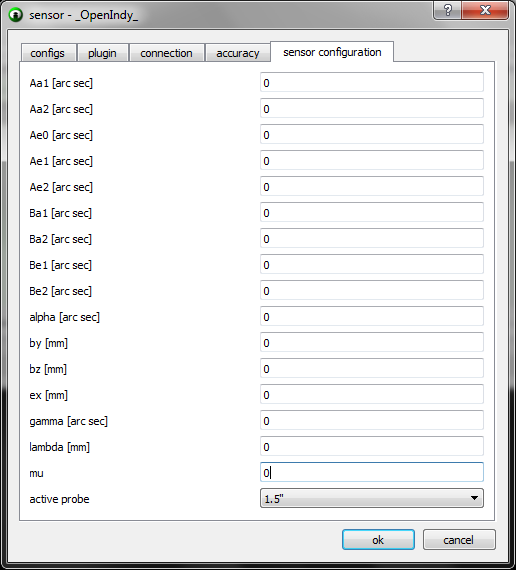
\includegraphics[scale=2.0]{bilder/sensorconfig}
	\caption{sensor configuration settings}
\end{figure}

Anschließend ist die Datei \texttt{TestUrsprungEcke.txt} mit den Sollwerten der Referenzpunkte zu importieren und 6 actual Punkt Feature mit identischem Namen anzulegen. Die Sollwerte sind auch in Tabelle \ref{tab:sollwerteecke} aufgelistet. Die Referenztemperatur für die Sollwerte ist $20^\circ\text{C}$ und das Material des Messobjektes ist Stahl mit einem Ausdehnungskoeffizienten, der Tabelle \ref{tab:ausdehnungskoeffizienten} zu entnehmen ist. Die Punkte werden einmal zu Beginn der Messaufgabe erfasst um die Transformationsparameter zwischen Instrumentensystem und Messobjektkoordinatensystem herzustellen. Anschließend sollen Neupunkte erfasst und auf ihre Lage geprüft werden. Dazu muss die Auswirkung der thermischen Ausdehnung auf deren Koordinaten kompensiert werden. Um die Messung übersichtlicher zu halten, werden 6 weitere actual Punkt Feature erzeugt mit den Namen $p1 - p6$. Die Sollwerte zu den Neupunkten sind in der Datei $\texttt{TestUrsprungEcke\_Neupunkte.txt}$ enthalten. Um die Messaufgabe übersichtlich zu halten, sind sie identisch mit den Sollwerten der Referenzpunkte und müssen vor Erzeugen der actual Punkt Feature importiert werden. Die Neupunkte werden ebenfalls mit den Beobachtungen, die auch für die Referenzpunkte verwendet wurden, erfasst. Die Beobachtungen zu den verschiedenen Ausdehnungszuständen sind den Tabellen \ref{tab:ausdehnung1} bis \ref{tab:ausdehnung4} zu entnehmen.\\
Da in dieser Messung eine gleichmäßige Ausdehnung in alle drei Koordinatenrichtungen simuliert wird, wird das Verfahren aus Kapitel \ref{sec:standardtempcomp} verwendet. Es wird angenommen, dass die Temperatur exakt bestimmt wurde und der Ausdehnungskoeffizient fehlerfrei ist.\\
Da dieses Verfahren gewählt wurde, muss vor Berechnung der Transformationsparameter um den Bezug der beiden Koordinatensysteme herzustellen, ein Movement mit der aktuellen Temperatur und dem Material angelegt werden, das bereits für die erste Beobachtung gültig ist. Die Temperatur während den ersten Messung beträgt $25^\circ\text{C}$. Deshalb werden die Beobachtungen aus Tabelle \ref{tab:ausdehnung1} mit dem \texttt{move Befehl} dem Pseudo Tracker übergeben und anschließend mit \texttt{measure} in das jeweilige Feature gemessen.\\
Die Messwerte wurden so erzeugt, dass sie einen Sensorstandpunkt von x = -1.0m, y = -1.0m und z = 1.0m im Objektkoordinatensystem darstellen.

\begin{figure}[h]
\label{fig:trafoParamausdehnung1ohnecomp}
\centering
	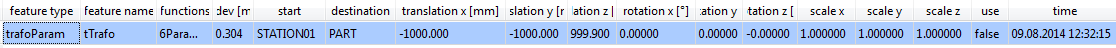
\includegraphics[scale=1.7]{bilder/Testmessung/ursprungecke/trafoParamausdehnung1ohnecomp}
	\caption{Transformationsparameter ohne Anwendung des Movements}
\end{figure}

Wie Grafik \ref{fig:trafoParamausdehnung1ohnecomp} zu entnehmen ist, hat die unkompensierte Ausdehnung des Messobjektes Einfluss auf die Transformationsparameter und wirkt sich bei der 6 Parameter Transformation in dieser Messung auf die Translation der z Komponente aus.

\begin{figure}[h]
\label{fig:trafoParamausdehnung1}
\centering
	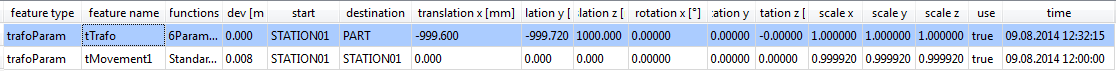
\includegraphics[scale=1.7]{bilder/Testmessung/ursprungecke/trafoParamausdehnung1}
	\caption{Transformation mit Anwendung des Movements und Ausdehnungsursprung bei (0.0m;0.0m;0.0m)}
\end{figure}

Bei Verwendung eines Movements bei der Berechnung der 6 Parameter Transformation wird die Ausdehnung zwar kompensiert, jedoch werden die Koordinaten des Messobjektes, aufgrund der Wahl des falschen Ausdehnungsursprunges, in der x- und y- Lage verschoben, was sich in den Translationen der Transformation widerspiegelt.

\begin{figure}[h]
\label{fig:trafoParamausdehnung1ausdurspr}
\centering
	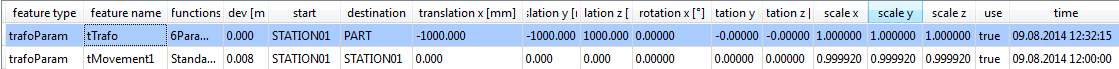
\includegraphics[scale=1.7]{bilder/Testmessung/ursprungecke/trafoParamausdehnung1ausdurspr}
	\caption{Transformation mit Anwendung des Movements und Ausdehnungsursprung bei (5.0m;3.5m;0.0m)}
\end{figure}

Grafik \ref{fig:trafoParamausdehnung1ausdurspr} zeigt die korrekten Transformationsparameter bei Wahl des richtigen Ausdehnungsursprunges, der bei diesem Messobjekt bei x = 5.0m, y = 3.5m und z = 0.0m liegt. Hier wird die Ausdehnung des Messobjektes kompensiert, ohne dass eine Verschiebung in der Lage stattfindet.

Würde man mit der 6 Parameter Transformation ohne Movement weiterarbeiten, so würden sich nach der Transformation der Beobachtungen in das Koordinatensystem folgende Restklaffen ergeben.
\newpage
\begin{figure}[h]
\label{fig:koordausdehnung1ohnecomp}
\centering
	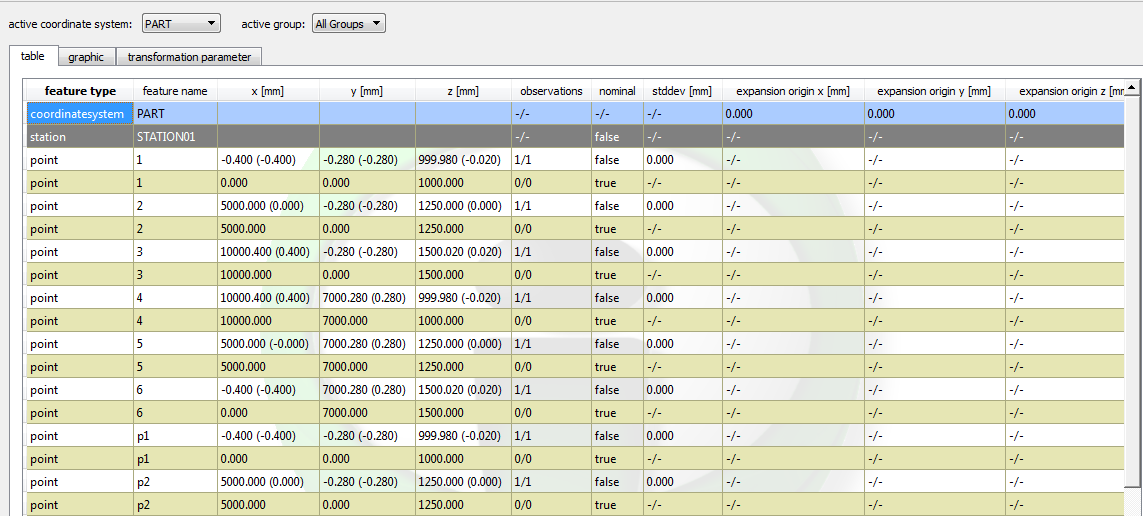
\includegraphics[scale=1.7]{bilder/Testmessung/ursprungecke/koordsausdehnung1ohnecomp}
	\caption{Restklaffen der transformierten Koordinaten ohne Movement}
\end{figure}
Wie in der Grafik ersichtlich wird, reicht die Transformation nicht aus, um die Ausdehnung des Messobjektes zu kompensieren und es verbleiben deutliche Restklaffen in den Koordinaten.\\
Aus diesem Grund ist es nötig die Transformation mit Movement aus Grafik \ref{fig:trafoParamausdehnung1} zu verwenden. Bei dieser Berechnung wird eine Kompensation der Ausdehnung in Richtung Koordinatenursprung durchgeführt.

\begin{figure}[H]
\label{fig:koordausdehnung1}
\centering
	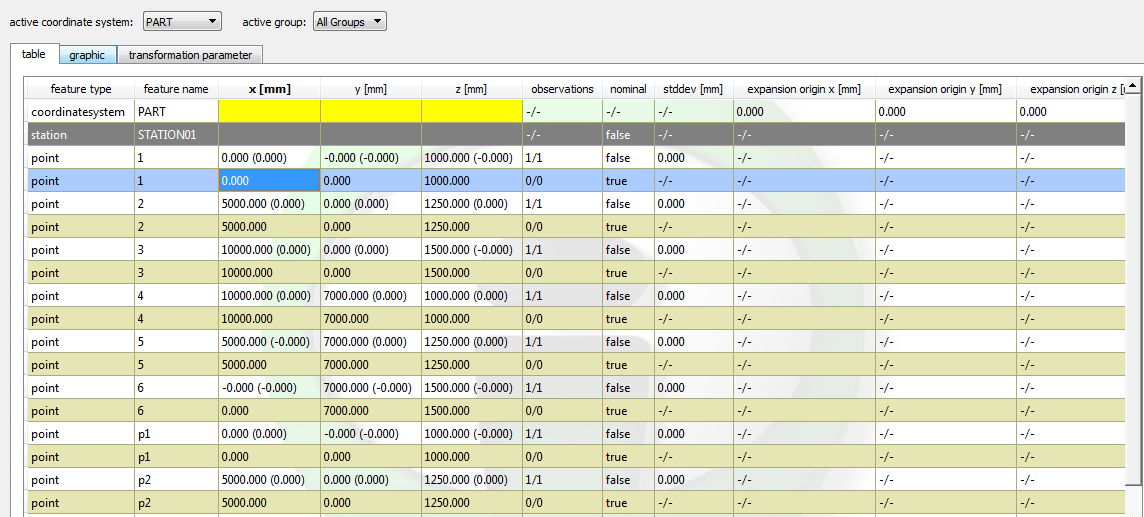
\includegraphics[scale=1.7]{bilder/Testmessung/ursprungecke/koordsausdehnung1}
	\caption{Restklaffen der zum Koordinatenursprung kompensierten Koordinaten}
\end{figure}

Die Restklaffen aus Grafik \ref{fig:koordausdehnung1} sind 0.0, jedoch liegt dies daran, dass der fälschlich angenommene Ausdehnungsursprung auch Einfluss auf die 6 Parameter Transformation hat. Die durch das Anwenden des Movements entstehende Translation steckt mit umgekehrten Vorzeichen in der 6 Parameter Transformation, da hier die Nominalwerte mit der Inverse des Maßstabes multipliziert wurden, um die Ist- Werte und Referenzwerte in den selben Zustand zu rechnen.\\
Geht man nun von einer weiteren Temperatursteigerung von $5^\circ\text{C}$ während der Messung aus, und erfasst die Punkte p1 - p6 mit den Beobachtungen aus \ref{tab:ausdehnung2} erneut, so sieht man, dass auch durch weiteres Anbringen des neuen Movements (siehe Grafik \ref{fig:trafoparamausdehnung2}), die Restklaffen nicht beseitigt werden können. Das neu erzeugte Movement soll die aktuellen Beobachtungen kompensieren.
\begin{figure}[H]
\label{fig:trafoparamausdehnung2}
\centering
	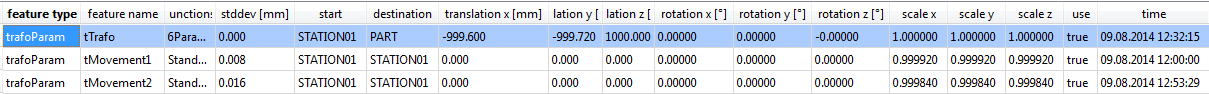
\includegraphics[scale=1.6]{bilder/Testmessung/ursprungecke/trafoParamausdehnung2}
	\caption{Transformationsparameter für $30^\circ\text{C}$ mit Korrektur zum Koordinatenursprung}
\end{figure}

Aufgrund des falsch gewählten Ausdehnungsursprunges, resultieren Restklaffen in der Größenordnung von mehreren $100\mu m$.

\begin{figure}[h]
\label{fig:koordausdehnung2}
\centering
	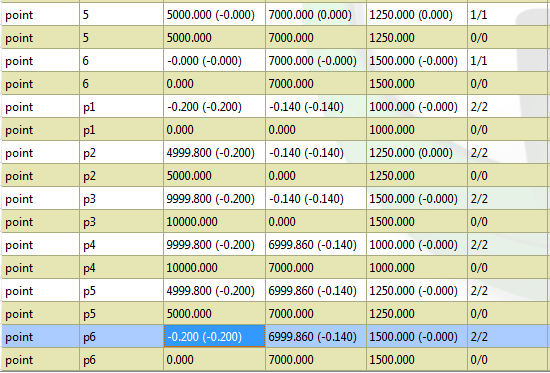
\includegraphics[scale=2.0]{bilder/Testmessung/ursprungecke/koordsausdehnung2}
	\caption{Restklaffen der zum Koordinatenursprung kompensierten Punkte bei $30^\circ\text{C}$}
\end{figure}

Setzt man im Vergleich zur zuvor beschriebenen Variante den Ausdehnungsursprung auf x = 5000.000mm, y = 3500.000mm und z = 0.000mm, so ergeben sich die nachfolgend dargestellten Ergebnisse.
\begin{figure}[h]
\label{fig:trafoparamausdehnung2ausdurspr}
\centering
	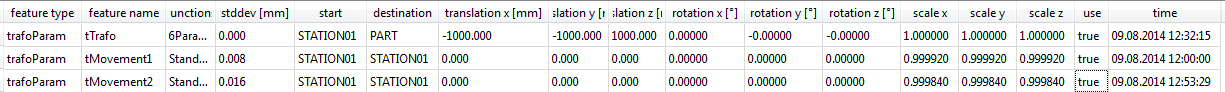
\includegraphics[scale=1.5]{bilder/Testmessung/ursprungecke/trafoParamausdehnung2ausdurspr}
	\caption{Transformationsparameter bei Ausdehnungsursprung x=5m, y=3.5m, z=0.0m}
\end{figure}

Die Anwendung dieser Transformationsparameter und Movements führt zu folgenden Restklaffen.

\begin{figure}[H]
\label{fig:koordausdehnung2ausdurspr}
\centering
	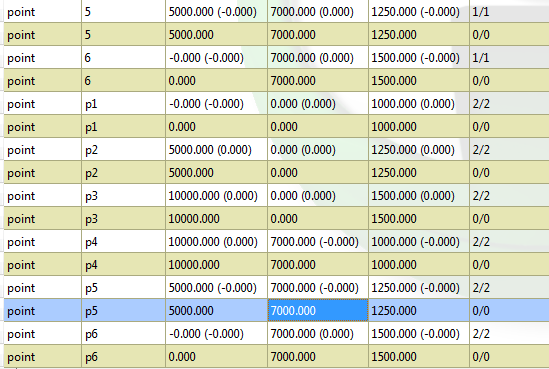
\includegraphics[scale=2.0]{bilder/Testmessung/ursprungecke/koordsausdehnung2ausdurspr}
	\caption{Restklaffen der zum Ausdehnungsursprung kompensierten Punkte}
\end{figure}

Wie durch Grafik \ref{fig:koordausdehnung2ausdurspr} gezeigt wird, hat die Wahl des Koordinatenursprungs großen Einfluss auf die Ergebnisse der Temperaturkompensation. Bei Wahl des falschen Ausdehnungsursprunges ist es nicht möglich die Restklaffen zu kompensieren. Bei Wahl des korrekt Ausdehnungsursprunges sind diese, bei Messung ohne Gerätefehler, vollständig eliminiert.\\
Da der exakte Ausdehnungsursprung meistens jedoch nicht bekannt ist, hilft es jedoch diesen näherungsweise anzugeben, und mit diesem genäherten Wert die Kompensation durchzuführen.\\

\begin{figure}[h]
\label{fig:trafoparamausdehnung2ausdursprnahe}
\centering
	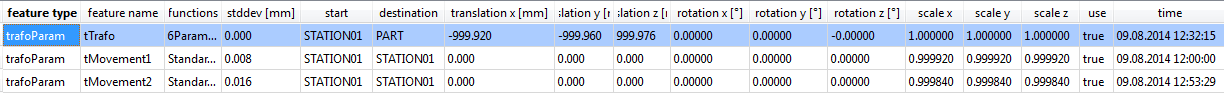
\includegraphics[scale=1.5]{bilder/Testmessung/ursprungecke/trafoParamausdehnung2ausdursprnahe}
	\caption{Transformationsparameter mit angenähertem Ausdehnungsursprung}
\end{figure}

Die Grafiken \ref{fig:trafoparamausdehnung2ausdursprnahe} und \ref{fig:koordausdehnung2ausdursprnahe} zeigen Transformationsparameter und Restklaffen der Messung mit einem nur näherungsweise bestimmten Ausdehnungsursprung. Die Koordinate des angenommenen und zur Kompensation verwendeten Ausdehnungsursprung liegt bei x=4000.000mm, y=3000.000mm und z=300.000mm. Vergleicht man die Grafik \ref{fig:koordausdehnung2} mit Grafik \ref{fig:koordausdehnung2ausdursprnahe}, so ist an den Restklaffen zu sehen, dass bereits die Annäherung des Ausdehnungsursprungs, zu deutlich besseren Ergebnissen führt. 

\begin{figure}[h]
\label{fig:koordausdehnung2ausdursprnahe}
\centering
	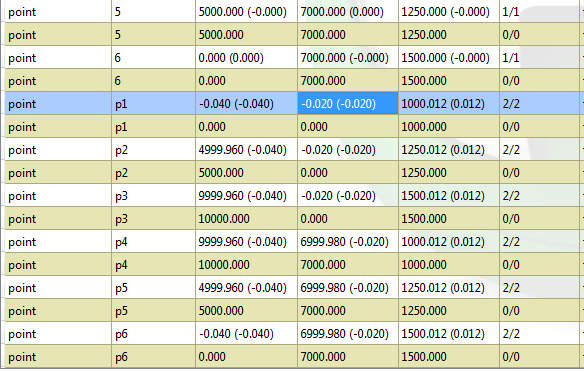
\includegraphics[scale=2.0]{bilder/Testmessung/ursprungecke/koordsausdehnung2ausdursprnahe}
	\caption{Restklaffen bei genähertem Ausdehnungsursprung}
\end{figure}

Würde man den Koordinatenursprung in die Mitte des Objektes und in die x-y- Ebene legen, so würde der tatsächliche Ausdehnungsursprung dem Koordinatenursprung entsprechen. Dies würde dazu führen, dass die Kompensation ohne Wahl des Ausdehnungsursprungs funktionieren würde und die richtigen Ergebnisse liefert. Sollwerte der Referenzpunkte und der zu prüfenden Neupunkte sind in den Dateien \texttt{TestUrsprungMitte.txt} und \texttt{$TestUrsprungMitte\_ Neupunkte.txt$} enthalten. Die Messung wird nicht weiter aufgeführt, da sie der obigen Variante mit Wahl des Ausdehnungsursprungs in x = 5000.000mm, y = 3500.000mm und z = 0.000mm entspricht.

\section{Erfassung der Ausdehnung eines Zylinders mit zwei Standpunkten}\label{sec:erfassungzylinder}

Die in Kapitel \ref{sec:einflussausdehnungsursprung} simulierte Messung mit Ausdehnung eines quaderähnlichen Messobjektes erfolgte mit einer gleichmäßigen Ausdehnung in allen drei Koordinatenachsen.\\ 
Da dieser Fall je nach Messobjekt nicht zutreffen ist, soll im nachfolgenden eine Messung simuliert werden, die nur eine Ausdehnung in x- Richtung enthält.\\
Aufgrund dieser Einschränkung ist das Standardverfahren aus Kapitel \ref{sec:standardtempcomp} nicht mehr anwendbar. Stattdessen muss die Ausdehnung über eine 9 Parameter Transformation erfasst werden, um die unterschiedliche Ausdehnung je Koordinatenachse erfassen zu können.

\begin{figure}[H]
\label{fig:zylinderuebersicht}
\centering
	\includegraphics[scale=1.0]{bilder/zylinder}
	\caption{Übersicht des Zylinders}
\end{figure}

Wie beschrieben, weißt der Zylinder nur eine Ausdehnung in x- Richtung auf. Sollwerte für die Referenzpunkte und für die, auf Lage zu prüfenden, Punkte sind in Tabelle \ref{tab:sollzylinder} aufgelistet.
\begin{figure}[h]
	\label{fig:zylinderausdehnung}
	\centering
	\subfigure[Axometrische Ansicht]{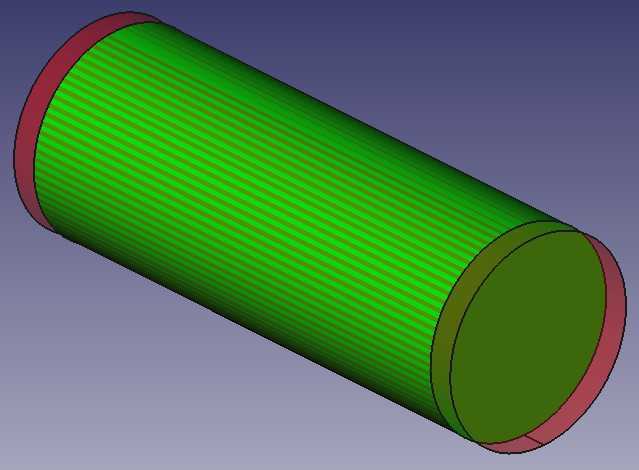
\includegraphics[width=0.4\textwidth]{FreeCADDaten/Zylinder/zylinderaxometrisch}}
	\subfigure[Seitenansicht]{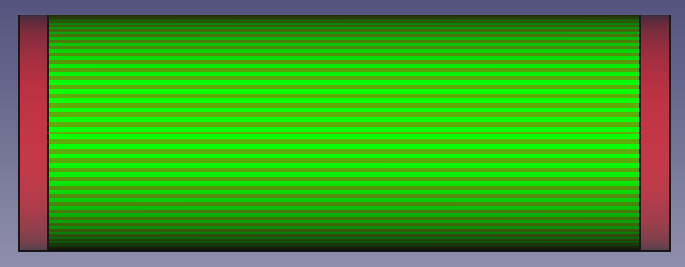
\includegraphics[width=0.4\textwidth]{FreeCADDaten/Zylinder/zylinderseitenansicht}} 
	\subfigure[Frontansicht]{
\includegraphics[width=0.15\textwidth]{FreeCADDaten/Zylinder/zylinderfrontansicht}}
	\caption[Ausdehnung des Zylinders]{Ausdehnung des Zylinders. grün = Referenz; rot = ausgedehnter Zustand)}
\end{figure}

Zur simulierten Messung sind folgende Annahmen und Bedingungen verwendet.\\
Der Zylinder ist auf einer Stahlplatte montiert, die die selben Maße wie der Zylinder aufweist. Die Referenzpunkte ref1 - ref4 liegen auf den Ecken der Platte und dienen zur Einmessung in das Objektkoordinatensystem.\\
Die Punkte 1 - 4 liegen auf den abgrenzenden Flächen des Zylinders und sind auf Solllage zu prüfen. Sie sollen im späteren Lauf für Bohrungen verwendet werden.\\
Aus Gründen der Sichtbarkeit muss die Messung mit zwei Standpunkten durchgeführt werden. Von Standpunkt 1 werden die Punkte ref1 - ref4 erfasst, um den Bezug zum Objektkoordinatensystem herzustellen.\\
Zusätzlich werden vier Verknüpfungspunkte auf dem Hallenboden angebracht und erfasst. Diese dienen dazu Standpunkte 2 mit Standpunkt 1 zu verknüpfen. Hierfür sind die Punkte com1 - com4 vorhanden und ebenfalls von Standpunkt 1 zu erfassen.\\
Da die Ausdehnung nur in eine Koordinatenachse stattfindet, werden die Movements mit einer 9 Parameter Transformation berechnet. Hierzu müssen mindestens drei Punkte am Messobjekt angebracht und bereits zu Beginn der Messung erfasst werden. Ihre Lageänderung durch die thermische Ausdehnung wird mit einer Transformation bestimmt und als Movement angewandt. Dazu dienen die Punkte p1 bis p4, die aus Gründen der Übersichtlichkeit die selben Koordinaten haben, wie die Punkte ref1 bis ref4.\\
Die Verteilung der Movement Punkte ist nicht sehr ideal, da die z- Achse nicht ausreichend abgesichert ist. Für diese Messung jedoch ist es ausreichend, da keine Ausdehnung in z- Richtung anzunehmen ist.\\
Da der Zylinder aus Stahl ist und die Temperatur zu Beginn der Messung $25^\circ\text{C}$ beträgt, werden die Messwerte aus Tabelle \ref{tab:zylinderausd1} mit dem Pseudo Tracker erfasst. Die Instrumentenfehler werden auch bei dieser Messung auf 0 gestellt, sodass sie keinen Einfluss auf die Ergebnisse haben.\\
Die Verknüpfungspunkte com1 - com4 sind auf dem Betonboden der Halle verklebt. Da Beton, im Vergleich zu Stahl, eine deutlich geringere Wärmeleitfähigkeit hat, vgl. Tabelle \ref{tab:wärmeleitfähigkeit}, ist anzunehmen, dass der Betonboden sich während der Messdauer nicht ausdehnt.

\begin{figure}[H]
\label{fig:s1transformiert}
\centering
	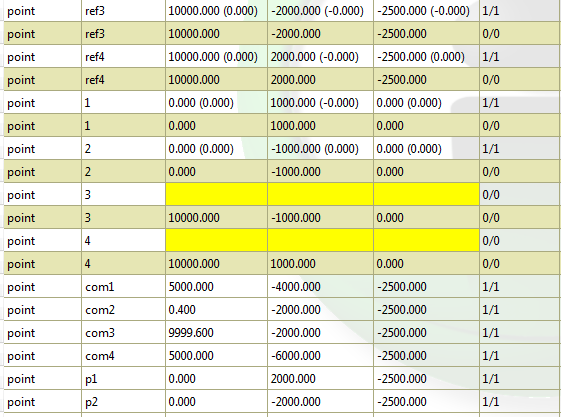
\includegraphics[scale=2.0]{bilder/Testmessung/zylinder/s1transformiert}
	\caption{Transformierte Koordinaten Standpunkt 1}
\end{figure}

Wie der Grafik zu entnehmen ist, sind die Punkte 3 und 4 nicht von Standpunkt 1 aus erfassbar. Die Punkte 1 und 2 entsprechen den Sollwerten.\\
Alle Beobachtungen von Standpunkt 2 wurden bei einer Materialtemperatur von $30^\circ\text{C}$ durchgeführt. 

\begin{figure}[H]
\label{fig:s2transformiert}
\centering
	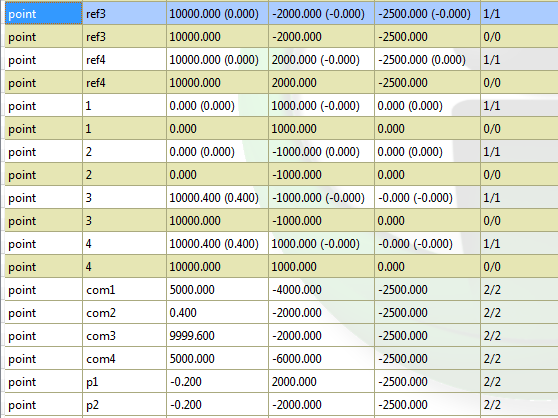
\includegraphics[scale=2.0]{bilder/Testmessung/zylinder/3u4ohneMovement}
	\caption{Transformierte Koordinaten Standpunkt 2}
\end{figure}

Die Restklaffen sind dadurch zu erklären, dass die Transformationen nur einen Temperaturunterschied von $5^\circ\text{C}$ kompensieren. Der aktuelle Temperaturunterschied muss durch Anbringen eines Movements von Standpunkt 2 kompensiert werden. Hierfür wird eine 9 Parameter Transformation zwischen den Beobachtungen aus den Movement Punkten p1 - p4 gerechnet und angewandt.

\begin{figure}[H]
\label{fig:s2Movement}
\centering
	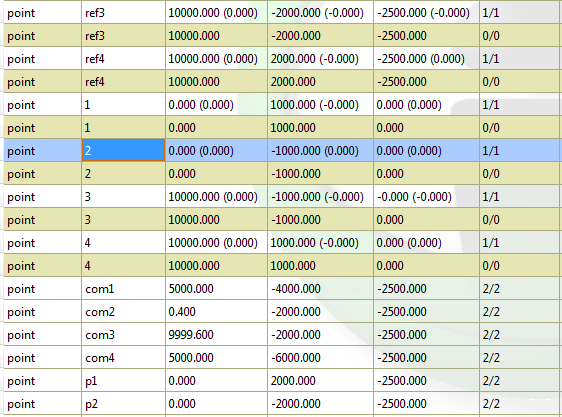
\includegraphics[scale=2.0]{bilder/Testmessung/zylinder/3u4mitMovement}
	\caption{Transformierte und korrigierte Koordinaten Standpunkt 2}
\end{figure}

Grafik \ref{fig:s2Movement} zeigt, dass auch dieser Temperaturunterschied vollständig durch die Transformationen kompensiert werden kann. Die Punkte 3 und 4 entsprechen auch ihren Sollwerten.

\begin{figure}[H]
\label{fig:transformationen}
\centering
	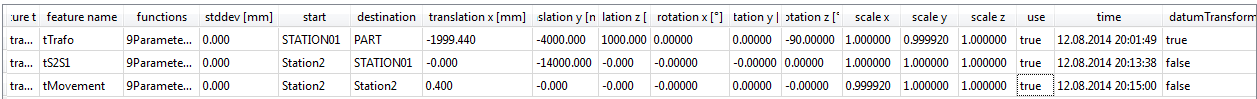
\includegraphics[scale=1.5]{bilder/Testmessung/zylinder/transformationen}
	\caption{Transformationsparameter der Messaufgabe}
\end{figure}

In Grafik \ref{fig:transformationen} sind die für diese Messaufgabe verwendeten Transformationsparameter.\\
\texttt{tTrafo} stellt den Bezug zwischen Instrumentensystem und Objektkoordinatensystem her. Hier ist die Temperaturkompensation bereits in den Maßstäben enthalten. \texttt{tS2S1} stellt die Beziehung zwischen den beiden Standpunkten her. Da sich die Verknüpfungspunkte nicht ausdehnen, ist der Maßstab dieser Transformation 1.000000. \\
Für den resultierenden Temperaturunterschied bei Standpunkt 2 wird ein Movement berechnet. Dieses kompensiert die um 5 Grad angestiegene Objekttemperatur.\\

Bei Anwendung dieses Verfahrens muss der Ausdehnungsursprung dem Koordinatenursprung entsprechen.\\
Die durch Anwendung des Maßstabes resultierende Verschiebung des Objektes wird bei dieser Variante durch die Translationen des Movements kompensiert. 

\section{Einfluss der Temperaturkompensation bei Simulationen}\label{sec:simulationen}

Der Einfluss der thermischen Ausdehnung und des Bezugspunkts wurde bei Nutzung der Simulationsschnittstelle von OpenIndy deutlich \cite{Lux2014}.

\begin{figure}[H]
\label{fig:simulationVorrichtung}
\centering
	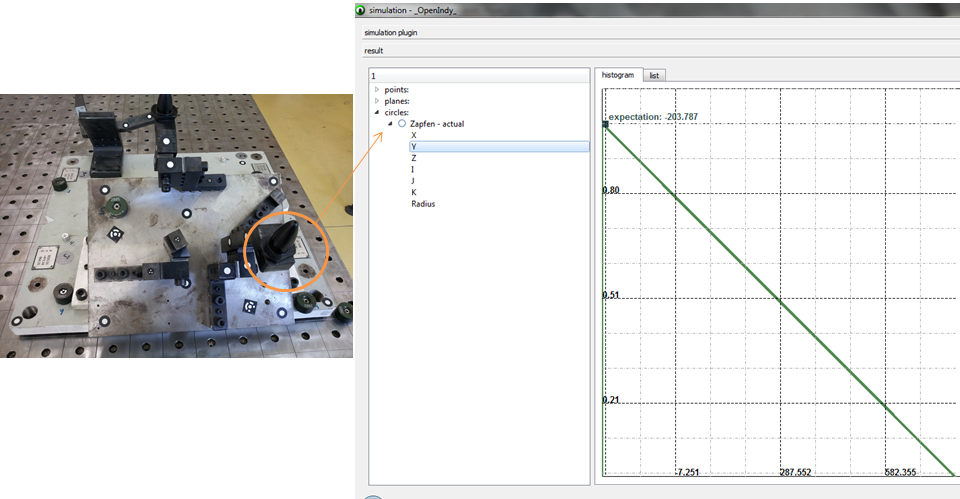
\includegraphics[scale=2.0]{bilder/vorrichtungsimulation}
	\caption{Vorrichtung und Ergebnis}
\end{figure}

In der Simulation wurden alle Fehlereinflüsse, außer die des Menschen, berücksichtigt. Die Korrektur der thermischen Ausdehnung erfolgt in der Simulation zum Koordinatenursprung.\\
Das Resultat der Simulation sind dreiecksverteilte Bestimmungsgrößen.
Die ermittelten Lageparameter unterscheiden sich deutlich von den tatsächlich gemessenen, was ein Zeichen für einen nicht identifizierbaren Einfluss ist.\\
Die Stichprobe wird in der Simulation auf normalverteilt oder gleichverteilt geprüft. Schlagen die Hypothesen fehl, so wird eine Dreiecksverteilung angenommen.\\
Eine Dreiecksverteilung wird meist bei einer spärlichen Anzahl an Daten verwendet, oder wenn keine konkrete Verteilung angenommen werden kann. Die Stichprobe ist somit nicht näher bestimmbar\footnote{\url{http://massmatics.de/merkzettel/index.php\#!869:Dreiecksverteilung} (Zugriff 13.08.2014)}.
Eine weitere Durchführung der Simulation, ohne Einfluss des Objekts führte zu normalverteilten Bestimmungsgrößen.\\

Eine erneute Messung mit einem Objekt, dessen Ausdehnungsursprung und Koordinatenursprung fast deckungsgleich sind, wurde in \cite{Lux2014} durchgeführt und führte zu plausiblen Ergebnissen.

\section{Zusammenfassung der Ergebnisse}

In den zuvor beschriebenen und durchgeführten Messungen zum Test der Verfahren zur Temperaturkompensation wurde gezeigt, dass es möglich ist die Ausdehnung des Messobjekts zu kompensieren. Je nach Wahl des Verfahrens ist darauf zu achten, welcher Ausdehnungsursprung anzugeben ist, um eine bestmögliche Kompensation zu erreichen. Die anzugebenden Werte sind beim jeweiligen Verfahren genannt. \\
Zu beachten ist, dass bei den Messungen das Messobjekt im thermischen Gleichgewicht war, also die Oberflächentemperatur mit der Kerntemperatur identisch war. Dies war eine Verallgemeinerung bei den simulierten Messungen, um die Komplexität zu verringern. In der Realität ist dies nicht anzunehmen, sodass die Kerntemperatur von der gemessenen Temperatur abweichen wird. Daraus resultieren Abweichungen, die nicht kompensiert werden können.\\
Ebenso ist zu beachten, dass in der Praxis Ungenauigkeiten in der Bestimmung der Temperatur enthalten sind. Diese wirken sich ebenfalls auf die Kompensation aus. Ein weiterer Einfluss ist, dass der Ausdehnungskoeffizient in der Regel auch nicht exakt bekannt ist und das Material von der Annahme abweichen wird.\\
Bei einer reellen Messung wird es auch aufgrund der Instrumentenfehler nicht möglich sein die Ausdehnung des Messobjekts vollständig zu kompensieren. Die Kompensation liefert jedoch deutlich bemerkbare Verbesserungen gegenüber einer unkompensierten Messung.

\chapter{Fazit und Ausblick}

Ziel der vorliegenden Masterarbeit war es ein Verfahren zur Temperaturkompensation von Messobjekten in der Industrievermessung zu erarbeiten und in OpenIndy zu implementieren. Die beiden implementierten Verfahren wurden auf Grundlage bereits existierender Verfahren gewählt und erarbeitet. Sie bieten die Möglichkeit zur Erfassung und Kompensation der Ausdehnung durch Temperaturbeobachtung oder durch Transformation über speziell gewählte Objektpunkte.\\
Im Vergleich zu bereits existierenden und kommerziellen Lösungen arbeiten die implementierten Verfahren nicht mit dem Koordinatenursprung des Messobjektes als Bezugspunkt zur Kompensation. Es wurde ein neues Attribut, der Ausdehnungsursprung, dem Koordinatensystem hinzugefügt. Dieser dient als Bezugspunkt für die Temperaturkompensation.\\
Im Vergleich zu existierenden Verfahren bietet dies die Möglichkeit auch fehlerfreie Kompensationen durchführen zu können, wenn der Koordinatenursprung vom Ausdehnungsursprung abweicht. Dies wurde in den Test gezeigt und belegt. Eine Schwierigkeit ist hier jedoch, dass der Ausdehnungsursprung zur Zeit von Hand eingegeben werden muss. Der Nutzer muss diesen also aus Plänen ermitteln, oder anhand des Messobjektes abschätzen. Besser wäre es hier, wenn dieser anhand von der Objektgeometrie oder anderen Beziehungen des Objektes ermittelt und automatisch gesetzt werden würde.\\
Des weiteren bieten die im Rahmen der Masterarbeit entwickelten Verfahren den Vorteil, dass sie transparent sind. Aufgrund der Open- Source- Lizenz von OpenIndy ist es so möglich Einblicke in die Algorithmik zu erlangen und deren Funktionsweise nachzuvollziehen. Ebenso könnten die Verfahren für den eigenen Bedarf abgeändert werden.
Zu beachten ist, dass die Genauigkeit der Verfahren von der Genauigkeit der Temperaturbeobachtung, der Korrektheit des Ausdehnungskoeffizienten und der Genauigkeit der bestimmten Punkte für die Transformation abhängig ist.\\

Zukünftig besteht die Möglichkeit, durch Einbringen einiger zusätzlicher Algorithmik, im Nachhinein einer Messung die Objekttemperatur oder dessen Ausdehnungskoeffizient anhand der Transformationen zurückzurechnen.
Hierzu müsste man die Maßstäbe aus den homogenen Transformationsmatrizen ausmultiplizieren. Anschließend muss das Gleichungssystem nach der gesuchten Größe, also der Objekttemperatur oder dem Ausdehnungskoeffizienten, umgestellt und gelöst werden.

Hierzu sei als kleine Übersicht $\beta$ der Maßstab, bzw. die Maßstabsmatrix der homogenen Transformation mit

\begin{equation}
\beta = 1 + (T_{actual} - T_{reference} * \alpha)
\end{equation} 

Aus der Messaufgabe würde sich für die verschiedenen Zeitpunkte eine Transformation ergeben, anhand der die Ausdehnung kompensiert wird.
Diese Gleichungen können dann zu einem großen Gleichungssystem zusammengefasst werden und für die Lösung des gesuchten Parameters verwendet werden.

\begin{equation}
\textbf{X}_{part} = \beta_{1}^{part} * \textbf{T}_{1}^{part} * \textbf{X}_{1}
\textbf{X}_{part} = \beta_{2}^{1} * \textbf{T}_{2}^{1} * \beta_{1}^{part} * \textbf{T}_{1}^{part} * \textbf{X}_{1}
\end{equation}

Die Anzahl der Gleichungen ist abhängig von der Anzahl der verwendeten Transformationsparameter je Messaufgabe.\\

Eine weitere Erweiterungsmöglichkeit bietet der Ausdehnungsursprung eines Messobjektes. Im aktuellen Stand besitzt jedes Messobjekt einen Ausdehnungsursprung, der für das gesamte Messobjekt gültig ist.\\
Bei komplexeren Messobjekten, die auch aus mehreren unterschiedlichen Materialien bestehen, wäre es von Vorteil mit unterschiedlichen Ausdehnungskoeffizienten zu arbeiten. Hier müsste den unterschiedlichen Objektgruppen, oder auch den einzelnen Feature des Messobjektes ein eigener Ausdehnungsursprung zugewiesen werden. Dies hätte den Vorteil, dass das Verhalten des Messobjektes möglichst detailgetreu nachgestellt werden kann. Häufig ist es der Fall, dass beispielsweise die x- Komponente eines Features auch durch die Ausdehnung des benachbarten Features beeinflusst wird. Dieses Problem könnte mit der Vergabe eines Ausdehnungsursprungs für jedes Feature gelöst werden.

\nocite{Keferstein2008}
\nocite{Dillinger2007}
\nocite{Graf1969}
\nocite{Zhu2008}

\bibliographystyle{alphadin}
\bibliography{masterarbeitLiteratur}

% Anhang
\appendix
\chapter{Vergleich der Transformationen}\label{chap:vergleichtrafo}

Der Einfluss der gewählten Transformation soll im nachfolgenden anhand einer Vergleichsmessung erläutert werden. Die Vergleichsmessung besteht aus der Erfassung von Referenzpunkten, für die Sollwerte existieren, im Labor der Sigma3D GmbH Mainz. Alle drei Transformationen werden mit den selben Beobachtungen berechnet und die Unterschiede in den Transformationsparametern werden gegenübergestellt.\\

%Tabelle mit Vergleich der Parameter.
\begin{table}[H]\label{tab:trafos}
\centering
\caption{Vergleich der Transformationen}
\rowcolors{3}{gray!10}{gray!50}

\begin{tabular}{cccc}
\toprule
\multicolumn{1}{p{2cm}|}{Parameter} &
\multicolumn{3}{c}{Helmert Transformation} \\
\multicolumn{1}{c|}{} &
\multicolumn{1}{c|}{6 Parameter} &
\multicolumn{1}{c|}{7 Parameter} &
\multicolumn{1}{c}{9 Parameter} \\
\midrule

\multicolumn{1}{c|}{Startsystem} &
\multicolumn{1}{c|}{STATION01} &
\multicolumn{1}{c|}{STATION01} &
\multicolumn{1}{c}{STATION01} \\

\multicolumn{1}{c|}{Zielsystem} &
\multicolumn{1}{c|}{PART} &
\multicolumn{1}{c|}{PART} &
\multicolumn{1}{c}{PART} \\

\multicolumn{1}{c|}{StdDev [mm]} &
\multicolumn{1}{c|}{0.220} &
\multicolumn{1}{c|}{0.039} &
\multicolumn{1}{c}{0.059} \\

\multicolumn{1}{c|}{tX [mm]} &
\multicolumn{1}{c|}{3309.725} &
\multicolumn{1}{c|}{3309.459} &
\multicolumn{1}{c}{3310.866} \\

\multicolumn{1}{c|}{tY [mm]} &
\multicolumn{1}{c|}{3300.497} &
\multicolumn{1}{c|}{3300.568} &
\multicolumn{1}{c}{3300.476} \\

\multicolumn{1}{c|}{tZ [mm]} &
\multicolumn{1}{c|}{1527.580} &
\multicolumn{1}{c|}{1527.576} &
\multicolumn{1}{c}{1527.592} \\

\multicolumn{1}{c|}{rX [$^\circ$]} &
\multicolumn{1}{c|}{-0.02298} &
\multicolumn{1}{c|}{-0.02298} &
\multicolumn{1}{c}{-0.02298} \\

\multicolumn{1}{c|}{rY [$^\circ$]} &
\multicolumn{1}{c|}{-0.64638} &
\multicolumn{1}{c|}{-0.64638} &
\multicolumn{1}{c}{-0.64638} \\

\multicolumn{1}{c|}{rZ [$^\circ$]} &
\multicolumn{1}{c|}{-176.32357} &
\multicolumn{1}{c|}{-176.32357} &
\multicolumn{1}{c}{-176.32357} \\

\multicolumn{1}{c|}{mX} &
\multicolumn{1}{c|}{1.000000} &
\multicolumn{1}{c|}{0.999919} &
\multicolumn{1}{c}{1.000342} \\

\multicolumn{1}{c|}{mY} &
\multicolumn{1}{c|}{1.000000} &
\multicolumn{1}{c|}{0.999919} &
\multicolumn{1}{c}{0.999921} \\

\multicolumn{1}{c|}{mZ} &
\multicolumn{1}{c|}{1.000000} &
\multicolumn{1}{c|}{0.999919} &
\multicolumn{1}{c}{0.999925} \\
\bottomrule

\end{tabular}
\end{table}

Wie der Tabelle zu entnehmen ist, hat bereits die Wahl der Transformation einen Einfluss auf die Genauigkeit der Messung und Kompensation. Die Messung wurde bei $21^\circ\text{C}$ durchgeführt, sodass die Maßstäbe als plausibel anzunehmen sind.\\

\begin{figure}[h]
	\label{fig:wandmessung}
	\centering
	\subfigure[Ausschnitt des Punktfelds]{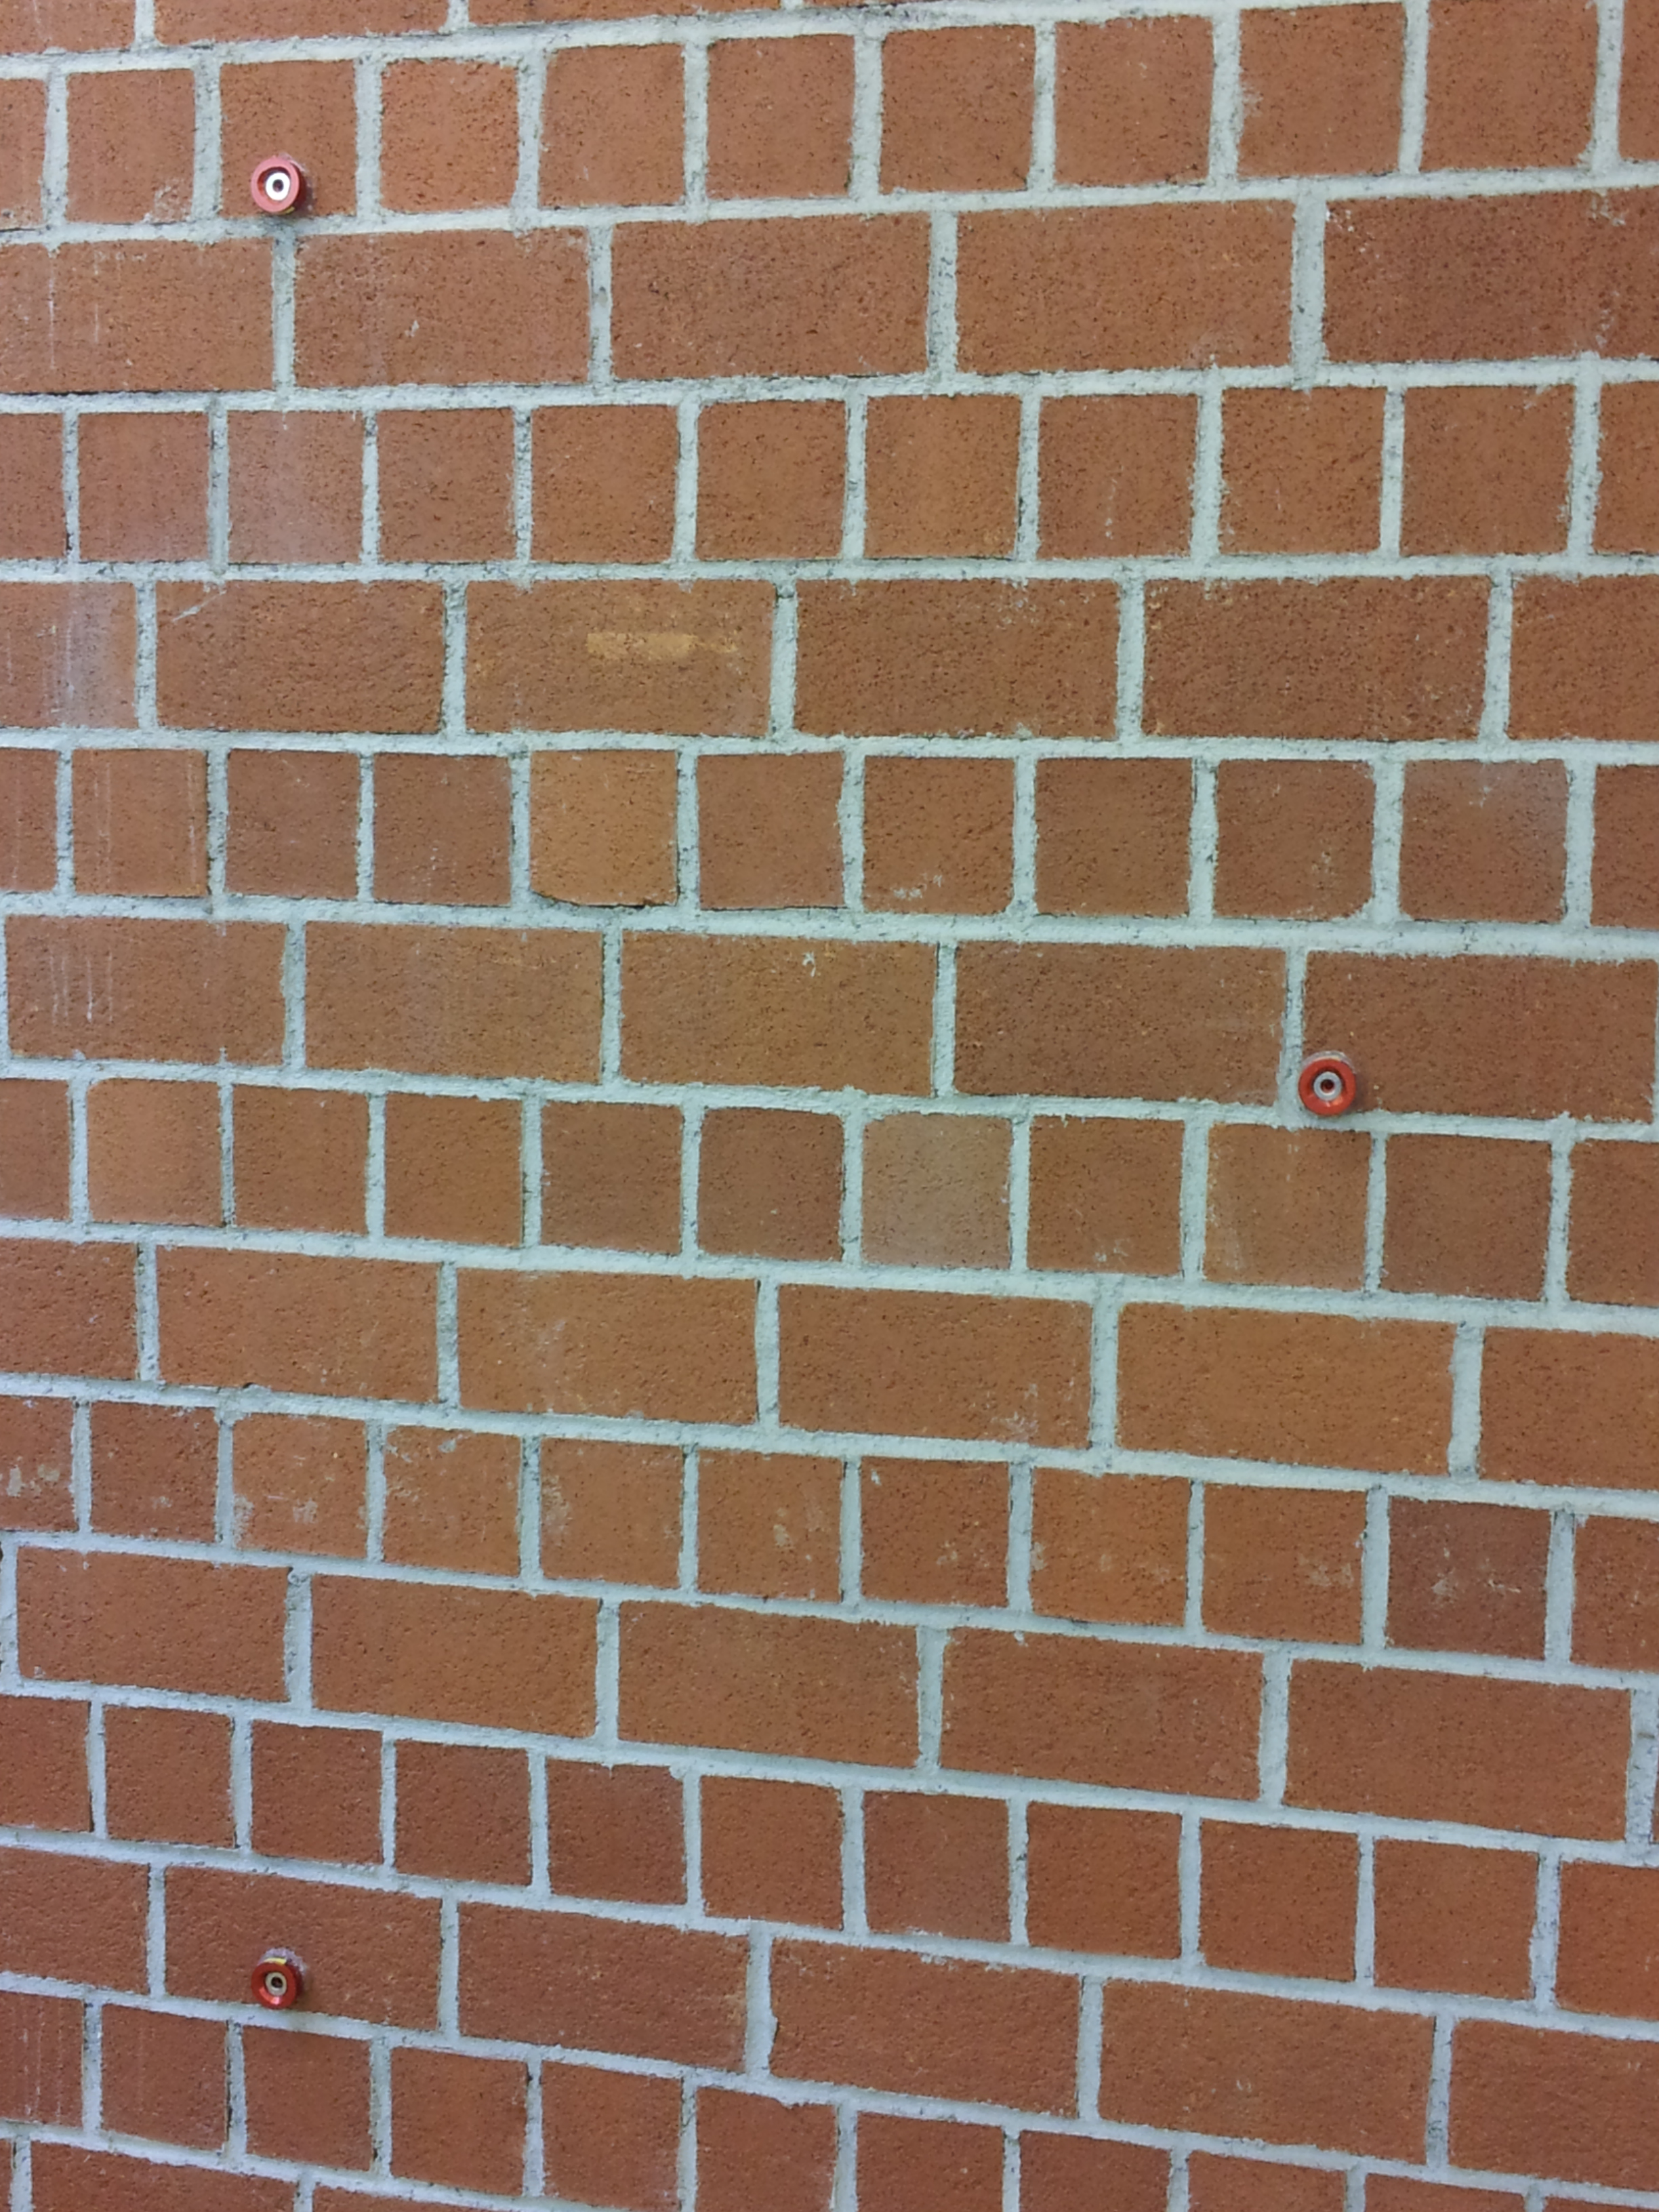
\includegraphics[width=0.4\textwidth]{bilder/wandPunkte}}
	\subfigure[Temperaturerfassung]{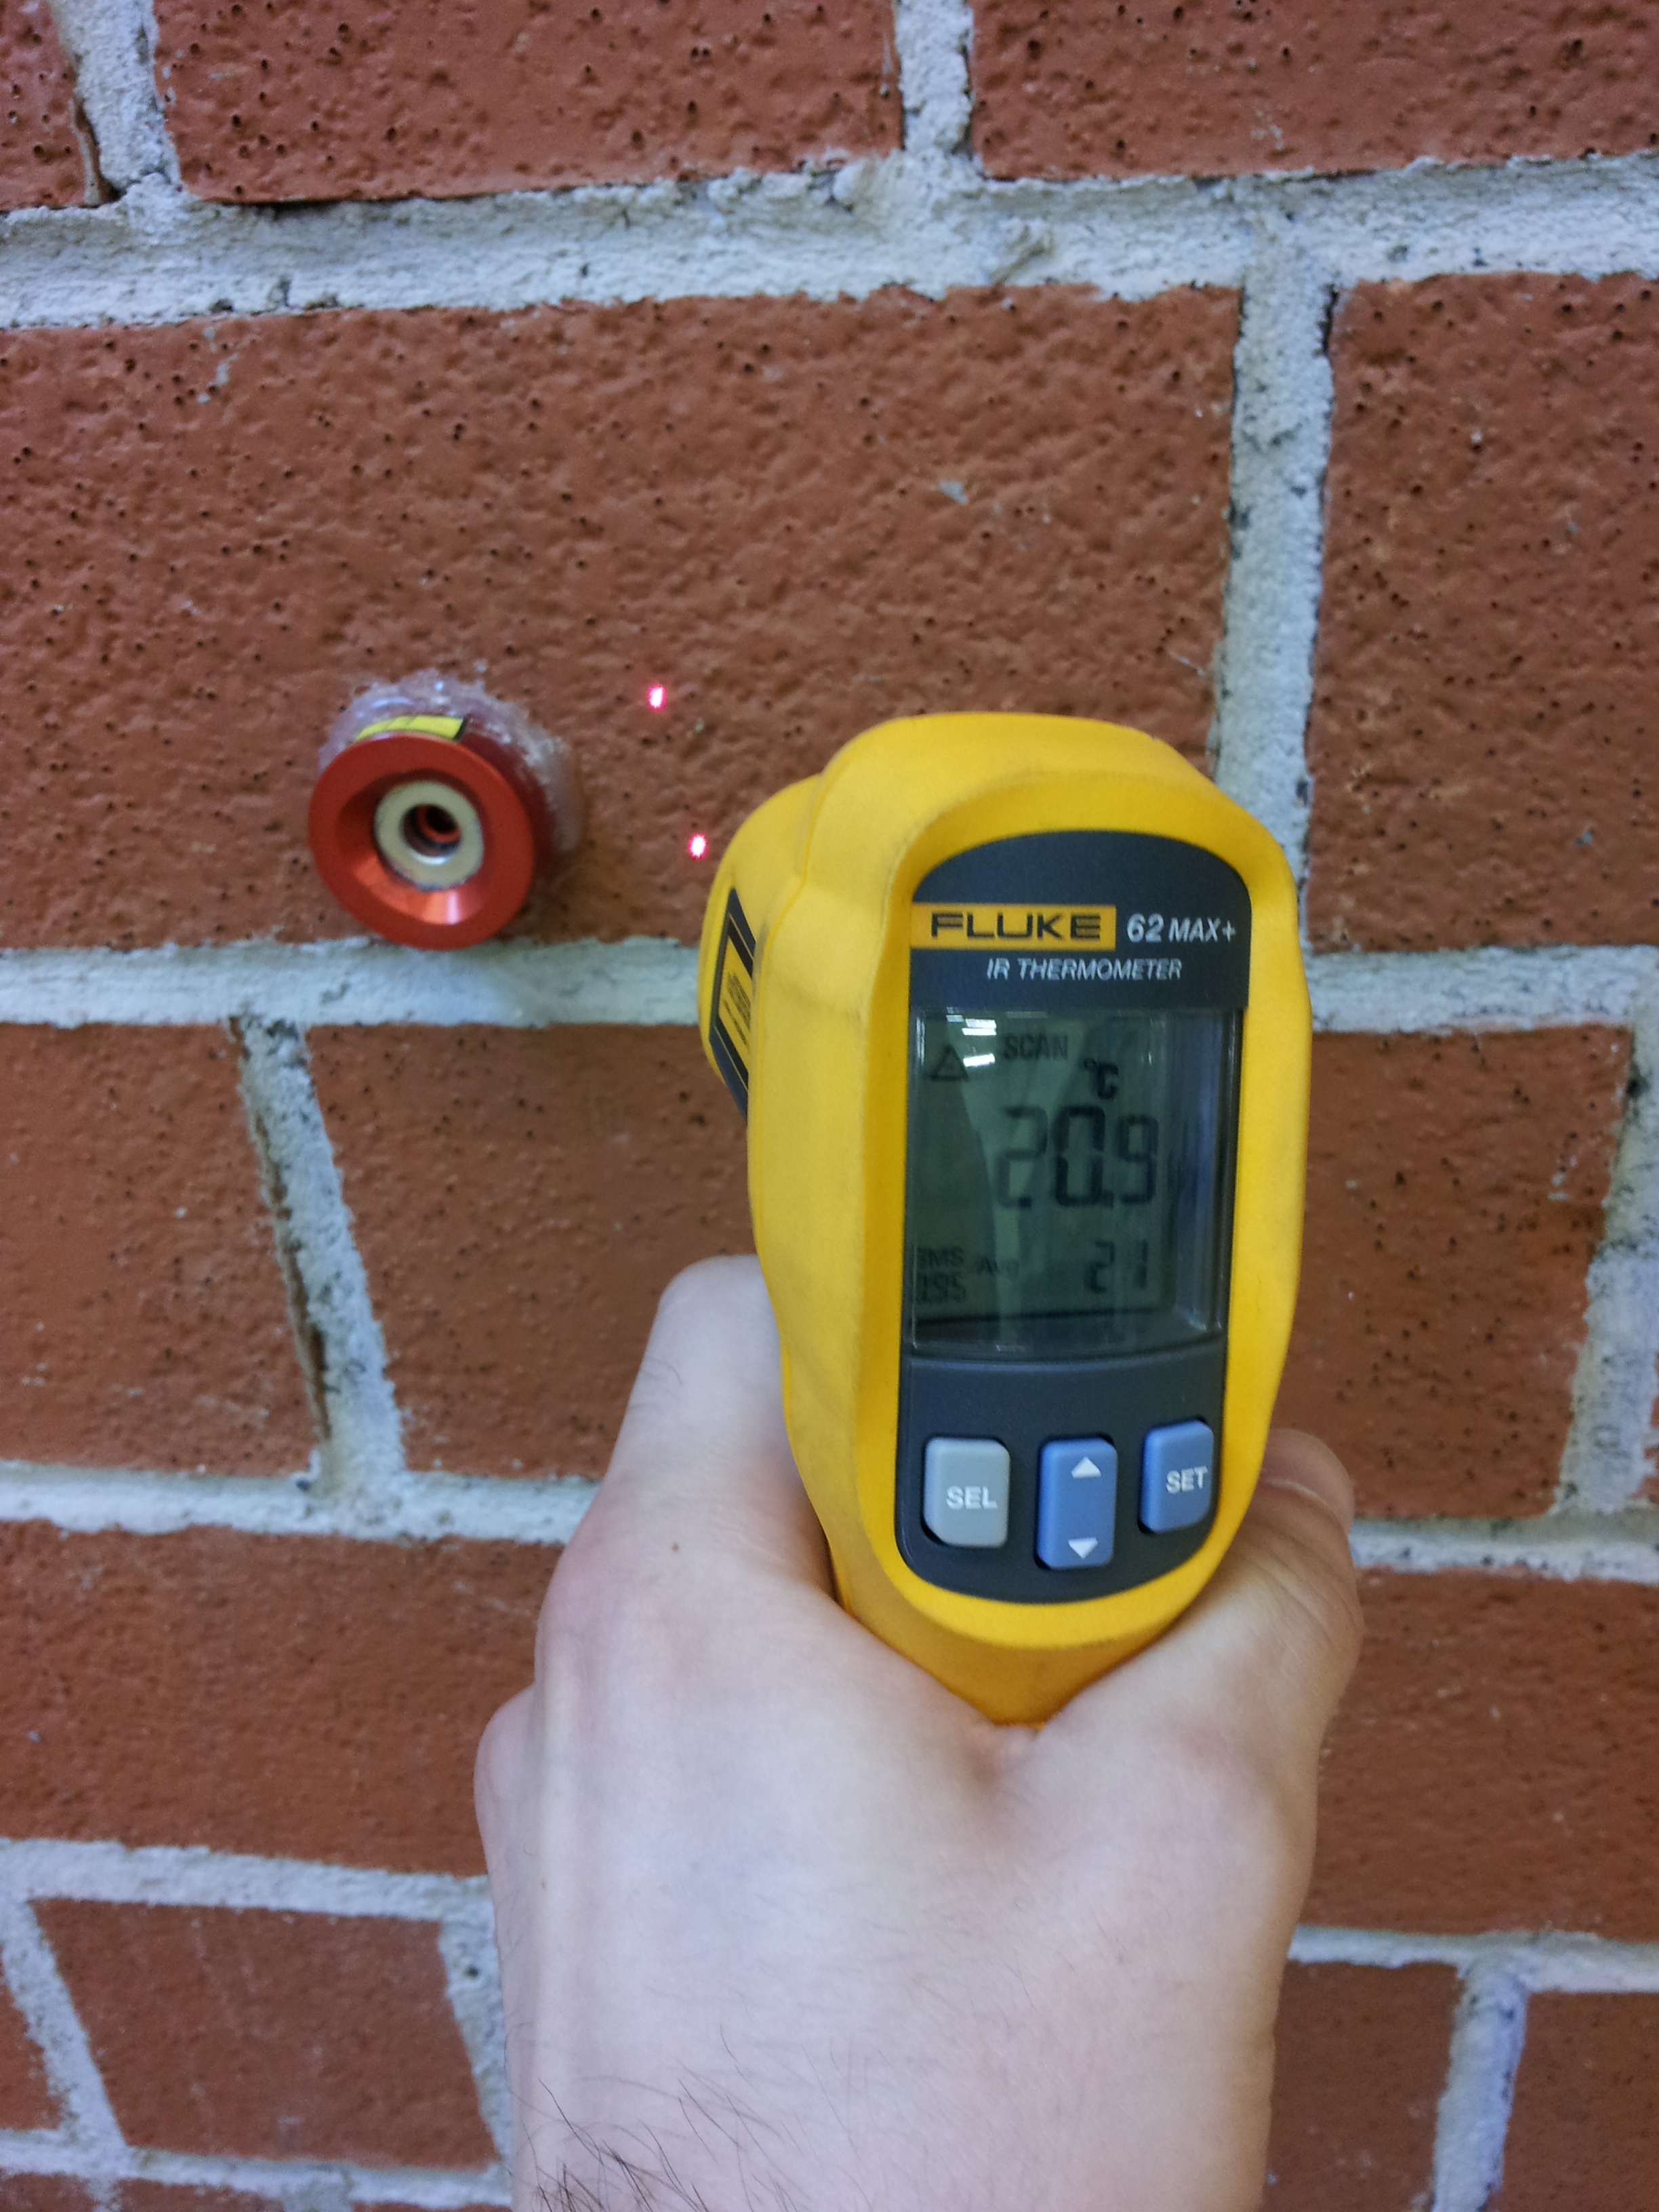
\includegraphics[width=0.4\textwidth]{bilder/temperaturmessung}}
	\caption{Einmessung in das Referenzpunktfeld}
\end{figure}

Des weiteren wird durch die Wahl der Transformation, die den Bezug zwischen Standpunkt und Objektkoordinatensystem herstellt, das spätere Verfahren zur Temperaturkompensation festgelegt. Da sich das Messobjekt meist nicht homogen in alle Richtungen ausdehnt, ist die 9 Parameter Helmert Transformation zu empfehlen, da diese die Ausdehnung in jede Koordinatenrichtung unterschiedlich erfasst und in den Maßstäben berücksichtigt. Nachfolgende Tabellen stellen die Restklaffen jeder einzelnen Transformation gegenüber.

%Tabelle Sollwerte !!!
\begin{table}[H]
\centering
\caption{Sollwerte der Referenzpunkte}

\rowcolors{3}{gray!10}{gray!50}
\begin{tabular}{ccccccc}
\toprule
\multicolumn{1}{p{1.5cm}|}{Name} &
\multicolumn{3}{c}{Soll-Koordinaten} \\
\multicolumn{1}{p{2cm}|}{} &
\multicolumn{1}{p{2cm}|}{X [mm]} &
\multicolumn{1}{p{2cm}|}{Y [mm]} &
\multicolumn{1}{p{2cm}}{Z [mm]} \\
\midrule

\multicolumn{1}{p{2cm}|}{10} &
\multicolumn{1}{p{2cm}|}{15.845} &
\multicolumn{1}{p{2cm}|}{1438.264} &
\multicolumn{1}{p{2cm}}{2130.126} \\

\multicolumn{1}{p{2cm}|}{11} &
\multicolumn{1}{p{2cm}|}{25.035} &
\multicolumn{1}{p{2cm}|}{1430.666} &
\multicolumn{1}{p{2cm}}{771.385} \\

\multicolumn{1}{p{2cm}|}{12} &
\multicolumn{1}{p{2cm}|}{22.824} &
\multicolumn{1}{p{2cm}|}{2218.675} &
\multicolumn{1}{p{2cm}}{1501.513} \\

\multicolumn{1}{p{2cm}|}{13} &
\multicolumn{1}{p{2cm}|}{21.866} &
\multicolumn{1}{p{2cm}|}{3896.552} &
\multicolumn{1}{p{2cm}}{1503.765} \\

\multicolumn{1}{p{2cm}|}{14} &
\multicolumn{1}{p{2cm}|}{24.491} &
\multicolumn{1}{p{2cm}|}{5158.900} &
\multicolumn{1}{p{2cm}}{1510.039} \\

\multicolumn{1}{p{2cm}|}{15} &
\multicolumn{1}{p{2cm}|}{20.776} &
\multicolumn{1}{p{2cm}|}{6446.732} &
\multicolumn{1}{p{2cm}}{2132.855} \\

\multicolumn{1}{p{2cm}|}{16} &
\multicolumn{1}{p{2cm}|}{23.480} &
\multicolumn{1}{p{2cm}|}{6438.500} &
\multicolumn{1}{p{2cm}}{1498.857} \\

\multicolumn{1}{p{2cm}|}{17} &
\multicolumn{1}{p{2cm}|}{27.691} &
\multicolumn{1}{p{2cm}|}{6425.388} &
\multicolumn{1}{p{2cm}}{766.588} \\

\bottomrule
\end{tabular}
\end{table}

%Tabelle Restklaffen 6Param
\begin{table}[H]\label{tab:restklaffen6p}
\centering
\caption{Restklaffen der 6 Parameter Transformation}

\rowcolors{3}{gray!10}{gray!50}
\begin{tabular}{ccccccc}
\toprule
\multicolumn{1}{p{1.5cm}|}{Name} &
\multicolumn{3}{c|}{Ist-Koordinaten} &
\multicolumn{3}{c}{Restklaffen} \\
\multicolumn{1}{p{2cm}|}{} &
\multicolumn{1}{p{2cm}|}{X [mm]} &
\multicolumn{1}{p{2cm}|}{Y [mm]} &
\multicolumn{1}{p{2cm}|}{Z [mm]} &
\multicolumn{1}{p{2cm}|}{X [mm]} &
\multicolumn{1}{p{2cm}|}{Y [mm]} &
\multicolumn{1}{p{2cm}}{Z [mm]} \\
\midrule

\multicolumn{1}{p{2cm}|}{10} &
\multicolumn{1}{p{2cm}|}{15.792} &
\multicolumn{1}{p{2cm}|}{1438.044} &
\multicolumn{1}{p{2cm}|}{2130.173} &
\multicolumn{1}{p{2cm}|}{0.053} &
\multicolumn{1}{p{2cm}|}{0.220} &
\multicolumn{1}{p{2cm}}{-0.047} \\

\multicolumn{1}{p{2cm}|}{11} &
\multicolumn{1}{p{2cm}|}{25.026} &
\multicolumn{1}{p{2cm}|}{1430.449} &
\multicolumn{1}{p{2cm}|}{771.331} &
\multicolumn{1}{p{2cm}|}{0.009} &
\multicolumn{1}{p{2cm}|}{0.217} &
\multicolumn{1}{p{2cm}}{0.054} \\

\multicolumn{1}{p{2cm}|}{12} &
\multicolumn{1}{p{2cm}|}{22.816} &
\multicolumn{1}{p{2cm}|}{2218.498} &
\multicolumn{1}{p{2cm}|}{1501.516} &
\multicolumn{1}{p{2cm}|}{0.008} &
\multicolumn{1}{p{2cm}|}{0.177} &
\multicolumn{1}{p{2cm}}{-0.003} \\

\multicolumn{1}{p{2cm}|}{13} &
\multicolumn{1}{p{2cm}|}{21.949} &
\multicolumn{1}{p{2cm}|}{3896.534} &
\multicolumn{1}{p{2cm}|}{1503.766} &
\multicolumn{1}{p{2cm}|}{-0.083} &
\multicolumn{1}{p{2cm}|}{0.018} &
\multicolumn{1}{p{2cm}}{-0.001} \\

\multicolumn{1}{p{2cm}|}{14} &
\multicolumn{1}{p{2cm}|}{24.591} &
\multicolumn{1}{p{2cm}|}{5159.000} &
\multicolumn{1}{p{2cm}|}{1510.041} &
\multicolumn{1}{p{2cm}|}{-0.100} &
\multicolumn{1}{p{2cm}|}{-0.100} &
\multicolumn{1}{p{2cm}}{-0.002} \\

\multicolumn{1}{p{2cm}|}{15} &
\multicolumn{1}{p{2cm}|}{20.747} &
\multicolumn{1}{p{2cm}|}{6446.919} &
\multicolumn{1}{p{2cm}|}{2132.912} &
\multicolumn{1}{p{2cm}|}{0.029} &
\multicolumn{1}{p{2cm}|}{-0.187} &
\multicolumn{1}{p{2cm}}{-0.057} \\

\multicolumn{1}{p{2cm}|}{16} &
\multicolumn{1}{p{2cm}|}{23.454} &
\multicolumn{1}{p{2cm}|}{6438.681} &
\multicolumn{1}{p{2cm}|}{1498.858} &
\multicolumn{1}{p{2cm}|}{0.026} &
\multicolumn{1}{p{2cm}|}{-0.181} &
\multicolumn{1}{p{2cm}}{-0.001} \\

\multicolumn{1}{p{2cm}|}{17} &
\multicolumn{1}{p{2cm}|}{27.632} &
\multicolumn{1}{p{2cm}|}{6425.553} &
\multicolumn{1}{p{2cm}|}{766.530} &
\multicolumn{1}{p{2cm}|}{0.059} &
\multicolumn{1}{p{2cm}|}{-0.165} &
\multicolumn{1}{p{2cm}}{0.058} \\

\bottomrule
\end{tabular}
\end{table}

%Tabelle Restklaffen 7Param
\begin{table}[H]\label{tab:restklaffen7p}
\centering
\caption{Restklaffen der 7 Parameter Transformation}

\rowcolors{3}{gray!10}{gray!50}
\begin{tabular}{ccccccc}
\toprule
\multicolumn{1}{p{1.5cm}|}{Name} &
\multicolumn{3}{c|}{Ist-Koordinaten} &
\multicolumn{3}{c}{Restklaffen} \\
\multicolumn{1}{p{2cm}|}{} &
\multicolumn{1}{p{2cm}|}{X [mm]} &
\multicolumn{1}{p{2cm}|}{Y [mm]} &
\multicolumn{1}{p{2cm}|}{Z [mm]} &
\multicolumn{1}{p{2cm}|}{X [mm]} &
\multicolumn{1}{p{2cm}|}{Y [mm]} &
\multicolumn{1}{p{2cm}}{Z [mm]} \\
\midrule

\multicolumn{1}{p{2cm}|}{10} &
\multicolumn{1}{p{2cm}|}{15.793} &
\multicolumn{1}{p{2cm}|}{1438.265} &
\multicolumn{1}{p{2cm}|}{2130.121} &
\multicolumn{1}{p{2cm}|}{0.052} &
\multicolumn{1}{p{2cm}|}{-0.001} &
\multicolumn{1}{p{2cm}}{0.005} \\

\multicolumn{1}{p{2cm}|}{11} &
\multicolumn{1}{p{2cm}|}{25.026} &
\multicolumn{1}{p{2cm}|}{1430.672} &
\multicolumn{1}{p{2cm}|}{771.388} &
\multicolumn{1}{p{2cm}|}{0.009} &
\multicolumn{1}{p{2cm}|}{-0.006} &
\multicolumn{1}{p{2cm}}{-0.003} \\

\multicolumn{1}{p{2cm}|}{12} &
\multicolumn{1}{p{2cm}|}{22.816} &
\multicolumn{1}{p{2cm}|}{2218.657} &
\multicolumn{1}{p{2cm}|}{1501.514} &
\multicolumn{1}{p{2cm}|}{0.008} &
\multicolumn{1}{p{2cm}|}{0.018} &
\multicolumn{1}{p{2cm}}{-0.001} \\

\multicolumn{1}{p{2cm}|}{13} &
\multicolumn{1}{p{2cm}|}{21.949} &
\multicolumn{1}{p{2cm}|}{3896.557} &
\multicolumn{1}{p{2cm}|}{1503.764} &
\multicolumn{1}{p{2cm}|}{-0.083} &
\multicolumn{1}{p{2cm}|}{-0.005} &
\multicolumn{1}{p{2cm}}{0.001} \\

\multicolumn{1}{p{2cm}|}{14} &
\multicolumn{1}{p{2cm}|}{24.591} &
\multicolumn{1}{p{2cm}|}{5158.921} &
\multicolumn{1}{p{2cm}|}{1510.039} &
\multicolumn{1}{p{2cm}|}{-0.100} &
\multicolumn{1}{p{2cm}|}{-0.021} &
\multicolumn{1}{p{2cm}}{0.000} \\

\multicolumn{1}{p{2cm}|}{15} &
\multicolumn{1}{p{2cm}|}{20.747} &
\multicolumn{1}{p{2cm}|}{6446.736} &
\multicolumn{1}{p{2cm}|}{2132.859} &
\multicolumn{1}{p{2cm}|}{0.029} &
\multicolumn{1}{p{2cm}|}{-0.004} &
\multicolumn{1}{p{2cm}}{-0.004} \\

\multicolumn{1}{p{2cm}|}{16} &
\multicolumn{1}{p{2cm}|}{23.454} &
\multicolumn{1}{p{2cm}|}{6438.498} &
\multicolumn{1}{p{2cm}|}{1498.856} &
\multicolumn{1}{p{2cm}|}{0.026} &
\multicolumn{1}{p{2cm}|}{0.002} &
\multicolumn{1}{p{2cm}}{0.001} \\

\multicolumn{1}{p{2cm}|}{17} &
\multicolumn{1}{p{2cm}|}{27.631} &
\multicolumn{1}{p{2cm}|}{6425.371} &
\multicolumn{1}{p{2cm}|}{766.588} &
\multicolumn{1}{p{2cm}|}{0.060} &
\multicolumn{1}{p{2cm}|}{0.017} &
\multicolumn{1}{p{2cm}}{0.000} \\

\bottomrule
\end{tabular}
\end{table}

%Tabelle Restklaffen 9Param
\begin{table}[h]\label{tab:restklaffen9p}
\centering
\caption{Restklaffen der 9 Parameter Transformation}

\rowcolors{3}{gray!10}{gray!50}
\begin{tabular}{ccccccc}
\toprule
\multicolumn{1}{p{1.5cm}|}{Name} &
\multicolumn{3}{c|}{Ist-Koordinaten} &
\multicolumn{3}{c}{Restklaffen} \\
\multicolumn{1}{p{2cm}|}{} &
\multicolumn{1}{p{2cm}|}{X} &
\multicolumn{1}{p{2cm}|}{Y} &
\multicolumn{1}{p{2cm}|}{Z} &
\multicolumn{1}{p{2cm}|}{X} &
\multicolumn{1}{p{2cm}|}{Y} &
\multicolumn{1}{p{2cm}}{Z} \\
\midrule

\multicolumn{1}{p{2cm}|}{10} &
\multicolumn{1}{p{2cm}|}{15.867} &
\multicolumn{1}{p{2cm}|}{1438.225} &
\multicolumn{1}{p{2cm}|}{2130.125} &
\multicolumn{1}{p{2cm}|}{-0.022} &
\multicolumn{1}{p{2cm}|}{0.009} &
\multicolumn{1}{p{2cm}}{0.001} \\

\multicolumn{1}{p{2cm}|}{11} &
\multicolumn{1}{p{2cm}|}{25.098} &
\multicolumn{1}{p{2cm}|}{1430.662} &
\multicolumn{1}{p{2cm}|}{771.385} &
\multicolumn{1}{p{2cm}|}{-0.063} &
\multicolumn{1}{p{2cm}|}{0.04} &
\multicolumn{1}{p{2cm}}{0.000} \\

\multicolumn{1}{p{2cm}|}{12} &
\multicolumn{1}{p{2cm}|}{22.869} &
\multicolumn{1}{p{2cm}|}{2218.650} &
\multicolumn{1}{p{2cm}|}{1501.514} &
\multicolumn{1}{p{2cm}|}{-0.045} &
\multicolumn{1}{p{2cm}|}{0.025} &
\multicolumn{1}{p{2cm}}{-0.001} \\

\multicolumn{1}{p{2cm}|}{13} &
\multicolumn{1}{p{2cm}|}{21.957} &
\multicolumn{1}{p{2cm}|}{3896.556} &
\multicolumn{1}{p{2cm}|}{1503.764} &
\multicolumn{1}{p{2cm}|}{-0.091} &
\multicolumn{1}{p{2cm}|}{-0.004} &
\multicolumn{1}{p{2cm}}{0.001} \\

\multicolumn{1}{p{2cm}|}{14} &
\multicolumn{1}{p{2cm}|}{24.566} &
\multicolumn{1}{p{2cm}|}{5158.924} &
\multicolumn{1}{p{2cm}|}{1510.039} &
\multicolumn{1}{p{2cm}|}{-0.075} &
\multicolumn{1}{p{2cm}|}{-0.024} &
\multicolumn{1}{p{2cm}}{0.000} \\

\multicolumn{1}{p{2cm}|}{15} &
\multicolumn{1}{p{2cm}|}{20.688} &
\multicolumn{1}{p{2cm}|}{6446.744} &
\multicolumn{1}{p{2cm}|}{2132.862} &
\multicolumn{1}{p{2cm}|}{0.088} &
\multicolumn{1}{p{2cm}|}{-0.012} &
\multicolumn{1}{p{2cm}}{-0.007} \\

\multicolumn{1}{p{2cm}|}{16} &
\multicolumn{1}{p{2cm}|}{23.394} &
\multicolumn{1}{p{2cm}|}{6438.507} &
\multicolumn{1}{p{2cm}|}{1498.856} &
\multicolumn{1}{p{2cm}|}{-0.086} &
\multicolumn{1}{p{2cm}|}{-0.007} &
\multicolumn{1}{p{2cm}}{0.001} \\

\multicolumn{1}{p{2cm}|}{17} &
\multicolumn{1}{p{2cm}|}{27.570} &
\multicolumn{1}{p{2cm}|}{6425.379} &
\multicolumn{1}{p{2cm}|}{766.583} &
\multicolumn{1}{p{2cm}|}{-0.121} &
\multicolumn{1}{p{2cm}|}{0.009} &
\multicolumn{1}{p{2cm}}{0.005} \\

\bottomrule
\end{tabular}
\end{table}

Wie den Tabellen \ref{tab:restklaffen6p} bis \ref{tab:restklaffen9p} zu entnehmen ist, sind die Restklaffen der 6 Parametertransformation am größten, da diese Transformation die Ausdehnung der Messpunkte aufgrund von Temperaturabweichungen zur Referenztemperatur nicht erfassen und kompensieren kann. Um die Genauigkeit dieser Messung zu verbessern, müsste ein Movement mit der aktuellen Temperatur und dem Material erzeugt und berücksichtigt werden. Die Differenz zwischen der 7 Parameter- und der 9 Parametertransformation sind vernachlässigbar klein. Die lässt auf eine homogene Ausdehnung der Wand in alle drei Koordinatenrichtungen deuten.\\
Der Maßstab für die x- Koordinate ist am signifikantesten und auch die Restklaffen der x- Koordinaten. Dies ist darauf zurückzuführen, dass die Punkte nahezu in der y- z- Ebene liegen.

\chapter{Sollwerte und Messwerte zu den Testmessungen}

Die Tabellen enthalten die Sollwerte und Messwerte zu den Testmessungen, die mit dem Pseudo- Tracker des Default PlugIns durchgeführt wurden. Das Messobjekt ist aus Stahl, dessen Ausdehnungskoeffizient Tabelle \ref{tab:ausdehnungskoeffizienten} zu entnehmen ist. Die Referenztemperatur beträgt $20^\circ\text{C}$.

%Tabelle Sollwerte Messobjekt Ursprung Ecke
\begin{table}[h]\label{tab:sollwerteecke}
\centering
\caption{Sollwerte des Messobjekts mit Ursprung in der Ecke}

\rowcolors{3}{gray!10}{gray!50}
\begin{tabular}{cccc}
\toprule
\multicolumn{1}{c|}{Name} &
\multicolumn{3}{c}{Soll-Koordinaten} \\
\multicolumn{1}{c|}{} &
\multicolumn{1}{c|}{X [mm]} &
\multicolumn{1}{c|}{Y [mm]} &
\multicolumn{1}{c}{Z [mm]} \\
\midrule

\multicolumn{1}{c|}{1} &
\multicolumn{1}{c|}{0.000} &
\multicolumn{1}{c|}{0.000} &
\multicolumn{1}{c}{1000.000} \\

\multicolumn{1}{c|}{2} &
\multicolumn{1}{c|}{5000.000} &
\multicolumn{1}{c|}{0.000} &
\multicolumn{1}{c}{1250.000} \\

\multicolumn{1}{c|}{3} &
\multicolumn{1}{c|}{10000.000} &
\multicolumn{1}{c|}{0.000} &
\multicolumn{1}{c}{1500.000} \\

\multicolumn{1}{c|}{4} &
\multicolumn{1}{c|}{10000.000} &
\multicolumn{1}{c|}{7000.000} &
\multicolumn{1}{c}{1000.000} \\

\multicolumn{1}{c|}{5} &
\multicolumn{1}{c|}{5000.000} &
\multicolumn{1}{c|}{7000.000} &
\multicolumn{1}{c}{1250.000} \\

\multicolumn{1}{c|}{6} &
\multicolumn{1}{c|}{0.000} &
\multicolumn{1}{c|}{7000.000} &
\multicolumn{1}{c}{1500.000} \\
\bottomrule
\end{tabular}
\end{table}


%Tabelle Sollwerte Messobjekt Ursprung Mitte
\begin{table}[h]\label{tab:sollwertemitte}
\centering
\caption{Sollwerte des Messobjekts mit Ursprung in der Mitte}

\rowcolors{3}{gray!10}{gray!50}
\begin{tabular}{cccc}
\toprule
\multicolumn{1}{c|}{Name} &
\multicolumn{3}{c}{Soll-Koordinaten} \\
\multicolumn{1}{c|}{} &
\multicolumn{1}{c|}{X [mm]} &
\multicolumn{1}{c|}{Y [mm]} &
\multicolumn{1}{c}{Z [mm]} \\
\midrule

\multicolumn{1}{c|}{1} &
\multicolumn{1}{c|}{-5000.000} &
\multicolumn{1}{c|}{-3500.000} &
\multicolumn{1}{c}{1000.000} \\

\multicolumn{1}{c|}{2} &
\multicolumn{1}{c|}{0.000} &
\multicolumn{1}{c|}{-3500.000} &
\multicolumn{1}{c}{1250.000} \\

\multicolumn{1}{c|}{3} &
\multicolumn{1}{c|}{5000.000} &
\multicolumn{1}{c|}{-3500.000} &
\multicolumn{1}{c}{1500.000} \\

\multicolumn{1}{c|}{4} &
\multicolumn{1}{c|}{5000.000} &
\multicolumn{1}{c|}{3500.000} &
\multicolumn{1}{c}{1000.000} \\

\multicolumn{1}{c|}{5} &
\multicolumn{1}{c|}{0.000} &
\multicolumn{1}{c|}{3500.000} &
\multicolumn{1}{c}{1250.000} \\

\multicolumn{1}{c|}{6} &
\multicolumn{1}{c|}{-5000.000} &
\multicolumn{1}{c|}{3500.000} &
\multicolumn{1}{c}{1500.000} \\
\bottomrule
\end{tabular}
\end{table}

Die Messwerte wurden Gleichung \ref{eq:deltaL} zur Berechnung der ausgedehnten Strecke berechnet und gleichmäßig auf positive und negative X- und Y- Achse addiert. Nur die Ausdehnung in Z wurde vollständig auf die positive Z- Achse addiert, da sich das Messobjekt wegen dem Boden nicht nach unten ausdehnen kann.
%Tabelle Messwerte 25Grad 1.STPKT
\begin{table}[h]\label{tab:ausdehnung1}
\centering
\caption{Messwert zu Referenzpunkten Standpunkt 1 bei $25^\circ\text{C}$}

\rowcolors{3}{gray!10}{gray!50}
\begin{tabular}{cccc}
\toprule
\multicolumn{1}{c|}{Name} &
\multicolumn{3}{c}{Soll-Koordinaten} \\
\multicolumn{1}{c|}{} &
\multicolumn{1}{c|}{X [mm]} &
\multicolumn{1}{c|}{Y [mm]} &
\multicolumn{1}{c}{Z [mm]} \\
\midrule

\multicolumn{1}{c|}{1} &
\multicolumn{1}{c|}{999.600} &
\multicolumn{1}{c|}{999.720} &
\multicolumn{1}{c}{0.080} \\

\multicolumn{1}{c|}{2} &
\multicolumn{1}{c|}{6000.000} &
\multicolumn{1}{c|}{999.720} &
\multicolumn{1}{c}{250.100} \\

\multicolumn{1}{c|}{3} &
\multicolumn{1}{c|}{11000.400} &
\multicolumn{1}{c|}{999.720} &
\multicolumn{1}{c}{500.120} \\

\multicolumn{1}{c|}{4} &
\multicolumn{1}{c|}{11000.400} &
\multicolumn{1}{c|}{8000.280} &
\multicolumn{1}{c}{0.080} \\

\multicolumn{1}{c|}{5} &
\multicolumn{1}{c|}{6000.000} &
\multicolumn{1}{c|}{8000.280} &
\multicolumn{1}{c}{250.100} \\

\multicolumn{1}{c|}{6} &
\multicolumn{1}{c|}{999.600} &
\multicolumn{1}{c|}{8000.280} &
\multicolumn{1}{c}{500.120} \\
\bottomrule
\end{tabular}
\end{table}

%Tabelle Messwerte 30Grad 1.STPKT
\begin{table}[h]\label{tab:ausdehnung2}
\centering
\caption{Messwert zu Referenzpunkten Standpunkt 1 bei $30^\circ\text{C}$}

\rowcolors{3}{gray!10}{gray!50}
\begin{tabular}{cccc}
\toprule
\multicolumn{1}{c|}{Name} &
\multicolumn{3}{c}{Soll-Koordinaten} \\
\multicolumn{1}{c|}{} &
\multicolumn{1}{c|}{X [mm]} &
\multicolumn{1}{c|}{Y [mm]} &
\multicolumn{1}{c}{Z [mm]} \\
\midrule

\multicolumn{1}{c|}{1} &
\multicolumn{1}{c|}{999.200} &
\multicolumn{1}{c|}{999.440} &
\multicolumn{1}{c}{0.160} \\

\multicolumn{1}{c|}{2} &
\multicolumn{1}{c|}{6000.000} &
\multicolumn{1}{c|}{999.440} &
\multicolumn{1}{c}{250.200} \\

\multicolumn{1}{c|}{3} &
\multicolumn{1}{c|}{11000.800} &
\multicolumn{1}{c|}{999.440} &
\multicolumn{1}{c}{500.240} \\

\multicolumn{1}{c|}{4} &
\multicolumn{1}{c|}{11000.800} &
\multicolumn{1}{c|}{8000.560} &
\multicolumn{1}{c}{0.160} \\

\multicolumn{1}{c|}{5} &
\multicolumn{1}{c|}{6000.000} &
\multicolumn{1}{c|}{8000.560} &
\multicolumn{1}{c}{250.200} \\

\multicolumn{1}{c|}{6} &
\multicolumn{1}{c|}{999.200} &
\multicolumn{1}{c|}{8000.560} &
\multicolumn{1}{c}{500.240} \\
\bottomrule
\end{tabular}
\end{table}

%Tabelle Messwerte 35Grad 2.STPKT
\begin{table}[h]\label{tab:ausdehnung3}
\centering
\caption{Messwert zu Referenzpunkten Standpunkt 2 bei $35^\circ\text{C}$}

\rowcolors{3}{gray!10}{gray!50}
\begin{tabular}{cccc}
\toprule
\multicolumn{1}{c|}{Name} &
\multicolumn{3}{c}{Soll-Koordinaten} \\
\multicolumn{1}{c|}{} &
\multicolumn{1}{c|}{X [mm]} &
\multicolumn{1}{c|}{Y [mm]} &
\multicolumn{1}{c}{Z [mm]} \\
\midrule

\multicolumn{1}{c|}{1} &
\multicolumn{1}{c|}{1998.800} &
\multicolumn{1}{c|}{1999.160} &
\multicolumn{1}{c}{1000.240} \\

\multicolumn{1}{c|}{2} &
\multicolumn{1}{c|}{7000.000} &
\multicolumn{1}{c|}{1999.160} &
\multicolumn{1}{c}{1250.300} \\

\multicolumn{1}{c|}{3} &
\multicolumn{1}{c|}{12001.200} &
\multicolumn{1}{c|}{1999.160} &
\multicolumn{1}{c}{1500.360} \\

\multicolumn{1}{c|}{4} &
\multicolumn{1}{c|}{12001.200} &
\multicolumn{1}{c|}{9000.840} &
\multicolumn{1}{c}{1000.240} \\

\multicolumn{1}{c|}{5} &
\multicolumn{1}{c|}{7000.000} &
\multicolumn{1}{c|}{9000.840} &
\multicolumn{1}{c}{1250.300} \\

\multicolumn{1}{c|}{6} &
\multicolumn{1}{c|}{1998.800} &
\multicolumn{1}{c|}{9000.840} &
\multicolumn{1}{c}{1500.360} \\
\bottomrule
\end{tabular}
\end{table}

%Tabelle Messwerte 40Grad 2.STPKT
\begin{table}[h]\label{tab:ausdehnung4}
\centering
\caption{Messwert zu Referenzpunkten Standpunkt 2 bei $40^\circ\text{C}$}

\rowcolors{3}{gray!10}{gray!50}
\begin{tabular}{cccc}
\toprule
\multicolumn{1}{c|}{Name} &
\multicolumn{3}{c}{Soll-Koordinaten} \\
\multicolumn{1}{c|}{} &
\multicolumn{1}{c|}{X [mm]} &
\multicolumn{1}{c|}{Y [mm]} &
\multicolumn{1}{c}{Z [mm]} \\
\midrule

\multicolumn{1}{c|}{1} &
\multicolumn{1}{c|}{1998.400} &
\multicolumn{1}{c|}{1998.880} &
\multicolumn{1}{c}{1000.320} \\

\multicolumn{1}{c|}{2} &
\multicolumn{1}{c|}{7000.000} &
\multicolumn{1}{c|}{1998.880} &
\multicolumn{1}{c}{1250.400} \\

\multicolumn{1}{c|}{3} &
\multicolumn{1}{c|}{12001.600} &
\multicolumn{1}{c|}{1998.880} &
\multicolumn{1}{c}{1500.480} \\

\multicolumn{1}{c|}{4} &
\multicolumn{1}{c|}{12001.600} &
\multicolumn{1}{c|}{9001.120} &
\multicolumn{1}{c}{1000.320} \\

\multicolumn{1}{c|}{5} &
\multicolumn{1}{c|}{7000.000} &
\multicolumn{1}{c|}{9001.120} &
\multicolumn{1}{c}{1250.400} \\

\multicolumn{1}{c|}{6} &
\multicolumn{1}{c|}{1998.400} &
\multicolumn{1}{c|}{9001.120} &
\multicolumn{1}{c}{1500.480} \\
\bottomrule
\end{tabular}
\end{table}

%Tabelle Sollwerte Zylinder
\begin{table}[h]\label{tab:sollzylinder}
\centering
\caption{Sollwerte Zylinder}

\rowcolors{3}{gray!10}{gray!50}
\begin{tabular}{cccc}
\toprule
\multicolumn{1}{c|}{Name} &
\multicolumn{3}{c}{Soll-Koordinaten} \\
\multicolumn{1}{c|}{} &
\multicolumn{1}{c|}{X [mm]} &
\multicolumn{1}{c|}{Y [mm]} &
\multicolumn{1}{c}{Z [mm]} \\
\midrule

\multicolumn{1}{c|}{ref1} &
\multicolumn{1}{c|}{0.000} &
\multicolumn{1}{c|}{2000.000} &
\multicolumn{1}{c}{-2500.000} \\

\multicolumn{1}{c|}{ref2} &
\multicolumn{1}{c|}{0.000} &
\multicolumn{1}{c|}{-2000.000} &
\multicolumn{1}{c}{-2500.000} \\

\multicolumn{1}{c|}{ref3} &
\multicolumn{1}{c|}{10000.000} &
\multicolumn{1}{c|}{-2000.000} &
\multicolumn{1}{c}{-2500.000} \\

\multicolumn{1}{c|}{ref4} &
\multicolumn{1}{c|}{10000.000} &
\multicolumn{1}{c|}{2000.000} &
\multicolumn{1}{c}{-2500.000} \\

\multicolumn{1}{c|}{1} &
\multicolumn{1}{c|}{0.000} &
\multicolumn{1}{c|}{0.000} &
\multicolumn{1}{c}{0.000} \\

\multicolumn{1}{c|}{2} &
\multicolumn{1}{c|}{0.000} &
\multicolumn{1}{c|}{-1000.000} &
\multicolumn{1}{c}{0.000} \\

\multicolumn{1}{c|}{3} &
\multicolumn{1}{c|}{10000.000} &
\multicolumn{1}{c|}{-1000.000} &
\multicolumn{1}{c}{0.000} \\

\multicolumn{1}{c|}{4} &
\multicolumn{1}{c|}{10000.000} &
\multicolumn{1}{c|}{1000.000} &
\multicolumn{1}{c}{0.000} \\
\bottomrule
\end{tabular}
\end{table}

%Tabelle Messwerte 25Grad Zylinder
\begin{table}[h]\label{tab:zylinderausd1}
\centering
\caption{Messwerte für den Zylinder von Standpunkt 1 bei $25^\circ\text{C}$}

\rowcolors{3}{gray!10}{gray!50}
\begin{tabular}{cccc}
\toprule
\multicolumn{1}{c|}{Name} &
\multicolumn{3}{c}{Koordinaten} \\
\multicolumn{1}{c|}{} &
\multicolumn{1}{c|}{X [mm]} &
\multicolumn{1}{c|}{Y [mm]} &
\multicolumn{1}{c}{Z [mm]} \\
\midrule

\multicolumn{1}{c|}{ref1} &
\multicolumn{1}{c|}{6000.000} &
\multicolumn{1}{c|}{-1999.600} &
\multicolumn{1}{c}{-3500.000} \\

\multicolumn{1}{c|}{ref2} &
\multicolumn{1}{c|}{2000.000} &
\multicolumn{1}{c|}{-1999.600} &
\multicolumn{1}{c}{-3500.000} \\

\multicolumn{1}{c|}{ref3} &
\multicolumn{1}{c|}{2000.000} &
\multicolumn{1}{c|}{-12000.4} &
\multicolumn{1}{c}{-3500.000} \\

\multicolumn{1}{c|}{ref4} &
\multicolumn{1}{c|}{6000.000} &
\multicolumn{1}{c|}{-12000.400} &
\multicolumn{1}{c}{-3500.000} \\

\multicolumn{1}{c|}{com1} &
\multicolumn{1}{c|}{0.000} &
\multicolumn{1}{c|}{-7000.000} &
\multicolumn{1}{c}{-3500.000} \\

\multicolumn{1}{c|}{com2} &
\multicolumn{1}{c|}{2000.000} &
\multicolumn{1}{c|}{-2000.000} &
\multicolumn{1}{c}{-3500.000} \\

\multicolumn{1}{c|}{com3} &
\multicolumn{1}{c|}{2000.000} &
\multicolumn{1}{c|}{-12000.000} &
\multicolumn{1}{c}{-3500.000} \\

\multicolumn{1}{c|}{com4} &
\multicolumn{1}{c|}{-2000.000} &
\multicolumn{1}{c|}{-7000.000} &
\multicolumn{1}{c}{-3500.000} \\

\multicolumn{1}{c|}{p1} &
\multicolumn{1}{c|}{6000.000} &
\multicolumn{1}{c|}{-1999.600} &
\multicolumn{1}{c}{-3500.000} \\

\multicolumn{1}{c|}{p2} &
\multicolumn{1}{c|}{2000.000} &
\multicolumn{1}{c|}{-1999.600} &
\multicolumn{1}{c}{-3500.000} \\

\multicolumn{1}{c|}{p3} &
\multicolumn{1}{c|}{2000.000} &
\multicolumn{1}{c|}{-12000.4} &
\multicolumn{1}{c}{-3500.000} \\

\multicolumn{1}{c|}{p4} &
\multicolumn{1}{c|}{6000.000} &
\multicolumn{1}{c|}{-12000.4} &
\multicolumn{1}{c}{-3500.000} \\

\multicolumn{1}{c|}{1} &
\multicolumn{1}{c|}{5000.000} &
\multicolumn{1}{c|}{-1999.600} &
\multicolumn{1}{c}{-1000.000} \\

\multicolumn{1}{c|}{2} &
\multicolumn{1}{c|}{3000.000} &
\multicolumn{1}{c|}{-1999.6} &
\multicolumn{1}{c}{-1000.000} \\
\bottomrule
\end{tabular}
\end{table}

%Tabelle Messwerte 30Grad Zylinder
\begin{table}[h]\label{tab:zylinderausd2}
\centering
\caption{Messwerte für den Zylinder von Standpunkt 2 bei $30^\circ\text{C}$}

\rowcolors{3}{gray!10}{gray!50}
\begin{tabular}{cccc}
\toprule
\multicolumn{1}{c|}{Name} &
\multicolumn{3}{c}{Koordinaten} \\
\multicolumn{1}{c|}{} &
\multicolumn{1}{c|}{X [mm]} &
\multicolumn{1}{c|}{Y [mm]} &
\multicolumn{1}{c}{Z [mm]} \\
\midrule

\multicolumn{1}{c|}{com1} &
\multicolumn{1}{c|}{0.000} &
\multicolumn{1}{c|}{7000.000} &
\multicolumn{1}{c}{-3500.000} \\

\multicolumn{1}{c|}{com2} &
\multicolumn{1}{c|}{2000.000} &
\multicolumn{1}{c|}{12000.000} &
\multicolumn{1}{c}{-3500.000} \\

\multicolumn{1}{c|}{com3} &
\multicolumn{1}{c|}{2000.000} &
\multicolumn{1}{c|}{2000.000} &
\multicolumn{1}{c}{-3500.000} \\

\multicolumn{1}{c|}{com4} &
\multicolumn{1}{c|}{-2000.000} &
\multicolumn{1}{c|}{7000.000} &
\multicolumn{1}{c}{-3500.000} \\

\multicolumn{1}{c|}{p1} &
\multicolumn{1}{c|}{6000.000} &
\multicolumn{1}{c|}{-12000.800} &
\multicolumn{1}{c}{-3500.000} \\

\multicolumn{1}{c|}{p2} &
\multicolumn{1}{c|}{2000.000} &
\multicolumn{1}{c|}{-12000.800} &
\multicolumn{1}{c}{-3500.000} \\

\multicolumn{1}{c|}{p3} &
\multicolumn{1}{c|}{2000.000} &
\multicolumn{1}{c|}{1999.200} &
\multicolumn{1}{c}{-3500.000} \\

\multicolumn{1}{c|}{p4} &
\multicolumn{1}{c|}{6000.000} &
\multicolumn{1}{c|}{1999.200} &
\multicolumn{1}{c}{-3500.000} \\

\multicolumn{1}{c|}{3} &
\multicolumn{1}{c|}{3000.000} &
\multicolumn{1}{c|}{1999.200} &
\multicolumn{1}{c}{-1000.000} \\

\multicolumn{1}{c|}{4} &
\multicolumn{1}{c|}{5000.000} &
\multicolumn{1}{c|}{1999.200} &
\multicolumn{1}{c}{-1000.000} \\

\bottomrule
\end{tabular}
\end{table}

\chapter*{Danksagung}

\begin{center}
Ich möchte meiner Familie danken, dass sie mich während meiner Masterarbeit und auch während meines gesamten Studiums unterstützt und motiviert haben.\\

Des weiteren gilt mein Dank Benedikt Rauls und Martin Lux für die Zusammenarbeit bei der Entwicklung von OpenIndy, sowie für die zahlreichen Diskussionen bezüglich der Thematik.\\

Zusätzlich möchte ich mich bei der Firma sigma3D für die fachliche Betreuung und Unterstützung, sowie die Bereitstellung der Ressourcen bedanken.
\end{center}
\end{document}